%\noindent
%\justifying
\setlength{\parskip}{1em}

This chapter discusses the experiments conducted in this thesis, evaluation metrics and results. The evaluation metrics like accuracy, precision, recall, confusion matrix and F1-score are discussed in section \ref{EvaluationMetrics}. These metrics are used to evaluate the domain gap between the distributions and quality of \ac{CycleGAN} generated document images. In section \ref{experiments} conducted experiments are explained along with training plots, confusion matrices and classification reports. Finally, in section \ref{results}, quantitative and qualitative results are discussed thoroughly along with the typical failure cases.

\section{Evaluation Metrics}\label{EvaluationMetrics}

%\subsection{Accuracy}
%\subsection{Precision and Recall}
%\subsection{F1-score}

In machine learning, there are numerous performance metrics to evaluate neural networks. Each evaluates different aspects of neural network performance. Hence, It is needed to have a specific set of performance metrics for a particular problem solved using neural networks. It's vital to evaluate the neural network's performance after training using testing data in order to determine its actual performance and generalization error on unseen data \cite{powers2020evaluation}. In this thesis, the performance of classifiers trained upon different data distributions determined using annotated real document images (test dataset). The popular classifier performance evaluation metrics are accuracy, precision, recall, confusion matrix and F1-score \cite{powers2020evaluation}. 


The testing dataset used to evaluate the classifiers is unbalanced, hence metrics like weighted average and macro average F1-scores are essential for the performance comparison of the classifiers trained on different data distributions. Accuracy is the most common and widely used metric to evaluate classifiers. It is the ratio of accurately classified data items to the total number of observations (equation \ref{accuracy}) \cite{vakili2020performance}. The precision is ``how many selected items are relevant"\footnotemark. ``To put it another way, out of the observations that an algorithm has predicted to be positive, how many of them are actually positive'' \cite{vakili2020performance}. ``The precision is the ratio of the number of true positives divided by the sum of the true positive and false positives''\footnotemark (equations \ref{precision}). The recall is ``how many relevant items are selected"\footnotemark[\value{footnote}]. ``To put it another way, out of the observations that are actually positive, how many of them have been predicted by the algorithm" \cite{vakili2020performance}. ``The recall is the ratio of the number of true positives divided by the sum of true positives and false negatives''\footnotemark[\value{footnote}] (equations \ref{recall}). In below equations \ref{accuracy},  \ref{precision} and \ref{recall} the $TP$ means true positives, $TN$ means true negatives, $FP$ means false positives and $FN$ means false negatives.



\footnotetext[1]{\url{https://en.wikipedia.org/wiki/Precision_and_recall} last access: \dcdate}
\footnotetext[2]{\url{https://machinelearningmastery.com/precision-recall-and-f-measure-for-imbalanced-classification/} last access: \dcdate}

\begin{equation}\label{accuracy}
\textit{Accuracy} = \frac{TP + TN}{TP +TN+ FP + FN}
\end{equation}

\begin{equation}\label{precision}
\textit{Precision} = \frac{TP}{TP + FP}
\end{equation}

\begin{equation}\label{recall}
\textit{Recall} = \frac{TP}{TP + FN}
\end{equation}

\newpage
The F1-score is the harmonic mean of the precision and recall (equation \ref{F1-score}). The weighted average F1-score is determined by first calculating the F1-score of each class separately and each multiplied by the weight (the number of true instances for each class) and finally added together, hence favoring the majority class\footnotemark. The equation \ref{Weightedf1-score} represents the weighted average F1-score. The macro average F1-score computes the unweighted mean of separate F1-score of each class. The macro average F1-score does not take label inbalance into account\footnotemark[\value{footnote}]. This leads to bigger penalization when the classifier does not perform well on minority classes. The equation \ref{macrof1-score} represents the macro average F1-score. In equations \ref{Weightedf1-score} and \ref{macrof1-score}, $N$ represents number of classes. More information about accuracy, precision, recall and F1-score can be found \href{https://en.wikipedia.org/wiki/Precision_and_recall}{here.}

\footnotetext{\url{https://scikit-learn.org/stable/modules/generated/sklearn.metrics.f1_score.html} last access: \dcdate}


\begin{equation}\label{F1-score}
\textit{F1-score} = \frac{2 \times precision \times recall}{precision + recall}
\end{equation}


\begin{equation}\label{macrof1-score} 
\textit{Macro average F1-score} =  \frac{F1_{class1} + F1_{class2}+ ... + F1_{classN}}{N}
\end{equation}


\begin{equation}\label{Weightedf1-score} 
\textit{Weighted average F1-score} =  \frac{F1_{class1} \times W_1 + F1_{class2} \times W_2 + ... + F1_{classN} \times W_N}{N}
\end{equation}

The confusion matrix is the most intuitive metric to determine the accuracy of the classifiers. It is a table that describes how well a classifier performs on a test dataset that is labeled or annotated. It is useful when the classifier has to classify more than two classes. The instances of the true class are represented at each row of the confusion matrix whereas the instances of predicted class probabilities are represented by each column or vice versa. In this thesis, the confusion matrix is extensively used to determine the performance of the classifiers trained on different data distributions to analyze domain gap and quality of \ac{CycleGAN} generated document images. More information about the confusion matrix can be found \href{https://en.wikipedia.org/wiki/Confusion_matrix}{here}.

%\footnotemark \footnotetext{\url{https://en.wikipedia.org/wiki/Confusion_matrix} last access: \dcdate}


\section{Experiments}\label{experiments}

In this thesis, three data distributions are considered for the experiments. The synthetic data distribution, faxified data distribution and \ac{CycleGAN} generated data distribution. Experiments are performed to analyze the domain gap between these data distributions and real data distribution. The experiment is conducted to analyze the domain gap between \ac{CycleGAN} generated data distribution and real data distribution, determines the quality of \ac{CycleGAN} generated document images, revealing how much they are close to the real document images. 

Now let's describe the conducted experiments briefly, a) Train a classifier on synthetic document images and its performance is evaluated on testing dataset (Annotated real document images, table \ref{table:testdataset}). b) Another classifier with the same architecture is trained on faxified document images and its performance is evaluated on the testing dataset. c) The \ac{CycleGAN} is trained for 20 epochs, using synthetic document images (Source domain $X$) and real document images (Target domain $Y$) and the checkpoint is saved at the end of every epoch. Once \ac{CycleGAN} training is finished, the saved model is loaded to generate images or transform synthetic document images into realistic document images. From the saved \ac{CycleGAN} model, generator $G$, retrieved, as it transforms synthetic document images into realistic document images (Source domain $X$ to Target domain $Y$, $G: X \rightarrow Y$). 100,000 synthetic document images transformed into realistic document images, generating a dataset of 100,000 \ac{CycleGAN} generated document images, with 10 classes and each class has 10000 images. d) Next, another classifier, with same architecture is trained on the \ac{CycleGAN} generated document images and its performance is evaluated on testing dataset. This experiment determines the quality of the images generated by \ac{CycleGAN}. Also, it indicates how well \ac{CycleGAN} was able to close the domain gap between synthetic data distribution and real data distribution. To put it another way, how well the \ac{CycleGAN} generated data distribution matched the real data distribution. As a whole, how similar \ac{CycleGAN} generated document images are to the real document images. In this thesis, the evaluation metrics like accuracy, weighted average F1-score and macro average F1-score \cite{lipton2014thresholding} are used to determine the performance of classifiers on testing dataset. The architecture of the classifier is illustrated in table \ref{table:ClassifierArchitecture}.


\subsection{Experiment Steps}
\begin{enumerate}
    \itemsep0em 
    \item Train a classifier using synthetic document images and evaluate its performance over testing dataset.
    \item Train a classifier using faxified document images and evaluate its performance over testing dataset.
    \item Train \ac{CycleGAN} using synthetic document images and real document images.
    \item Generate realistic document images using generator $G$ retrieved from the trained and saved \ac{CycleGAN} model.
    \item Train a classifier using \ac{CycleGAN} generated document images and evaluate its performance over testing dataset. This experiment reveals how well the \ac{CycleGAN} generated document images are generalizing to the real document images, eventually determining the quality of images generated by \ac{CycleGAN}.
    \item Compare the classification performance of the above three classifiers (trained on 3 different data distributions) on testing dataset and determine which distribution is closer to the real data distribution.
\end{enumerate}

%The domain gap between real data distribution and other three distributions like synthetic data distribution, faxified data distribution and \ac{CycleGAN} generated data distribution.The performance evaluation of a classifier trained upon \ac{CycleGAN} generated data distribution using annotated real document images describes, how close is the \ac{CycleGAN} generated data distribution to the real data distribution. Simply this approach determines the quality of the \ac{CycleGAN} generated document images compared to real document images.


\subsection{Training a Classifier on Synthetic Document Images}\label{trainingsyntheticclassifier}

The dataset of synthetic document images is created using templates (figure of sample \ref{fig:template}) and handwritten crops (figure of sample \ref{fig:keinwifi}) using the process mentioned in figure \ref{fig:InsertHandwrittenCrops}. This dataset consists of 100,000 document images, 10 classes and each class has 10000 images. In this experiment, a classifier is trained on synthetic document images dataset. The performance of this classifier is evaluated on testing dataset (Annotated real document images) to understand the domain gap between real data distribution and synthetic data distribution. The classification report in table \ref{table:SyntheticClassificationReport} states that the accuracy of this classifier on real document images is 25\%, macro average F1-score is 27\% and weighted average F1-score is 31\%. The obtained results conclude that there is a huge gap between real data distribution and synthetic data distribution. The confusion matrix is illustrated in figure \ref{fig:CMSyntheticDocumentImagesClassifier}. In which, it is visible that most of the images from the testing dataset were classified wrongly. Only test images from classes DE\_LY\_Arm\_2020-01 (support 44), DE\_LY\_Bein\_2019-01 (support 50) and DE\_LY\_Hand\_2020-01 (support 16) are classified correctly with a recall score of 50\%, 90\% and 44\% respectively. The epochs against accuracy and epochs against loss plots while training classifier on synthetic document images is illustrated in figure \ref{fig:SyntheticClassifierAcc} and \ref{fig:SyntheticClassifierLoss} respectively. The epochs against accuracy and epochs against loss plots while training classifier on synthetic document images is illustrated in figure \ref{fig:SyntheticClassifierAcc} and \ref{fig:SyntheticClassifierLoss} respectively.


\begin{figure}[H]
  \centering
  \begin{minipage}[b]{0.45\textwidth}
    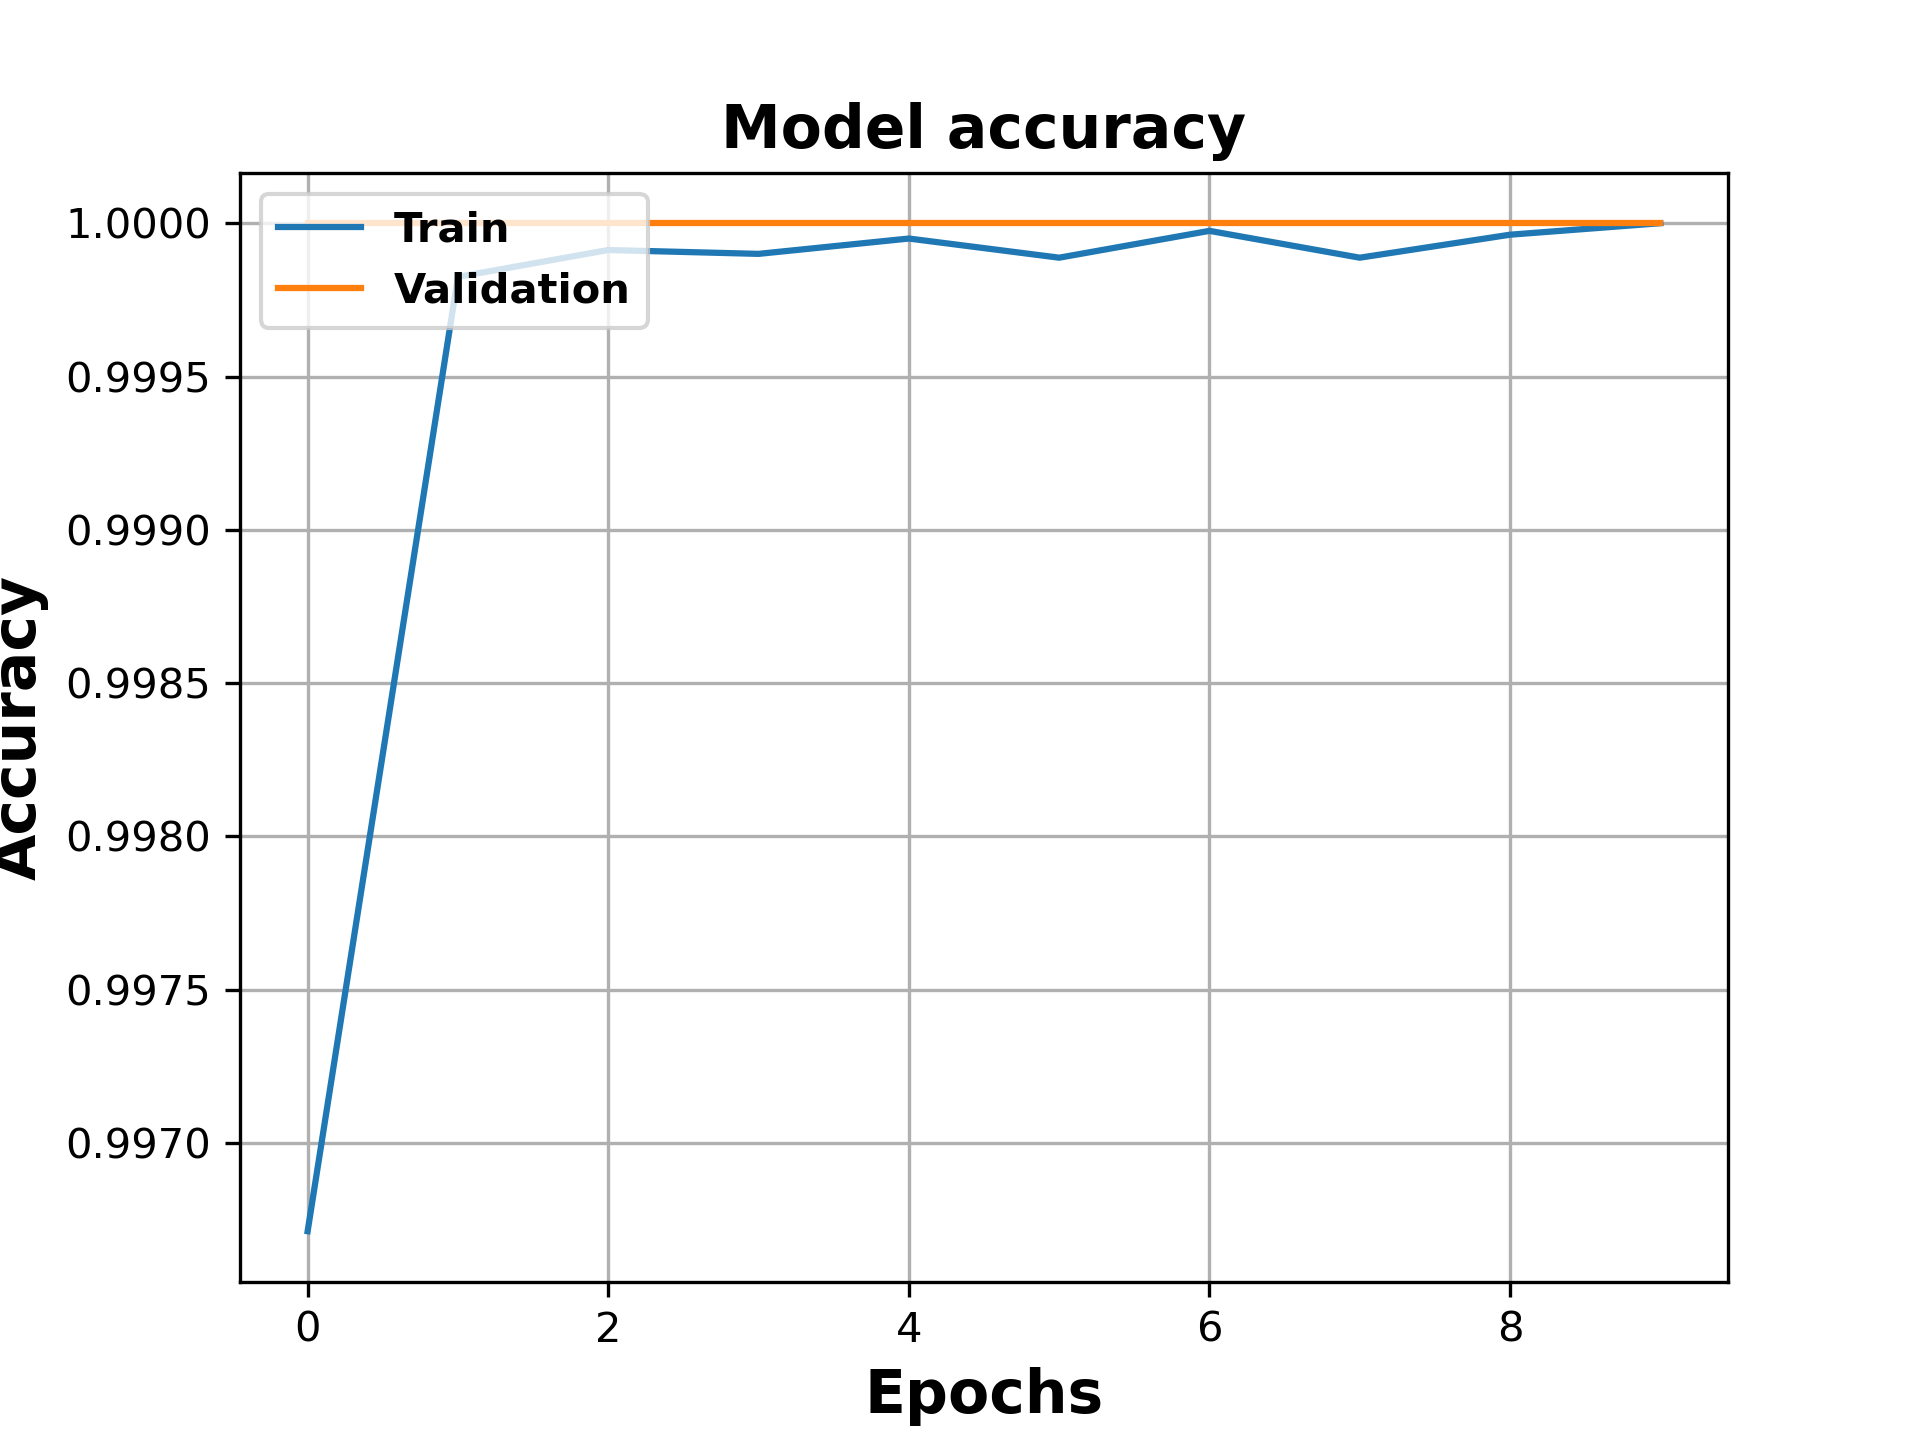
\includegraphics[width=\textwidth]{images/Evaluation/Synthetic_Data_Classifier_2021-05-31_16-40-33_Accuracy.png}
    \caption[Epochs vs. Accuracy plot during training a classifier on synthetic document images.]{Epochs vs. Accuracy plot during training a classifier on synthetic document images.}
    \label{fig:SyntheticClassifierAcc}
  \end{minipage}
  \hfill
  \begin{minipage}[b]{0.45\textwidth}
    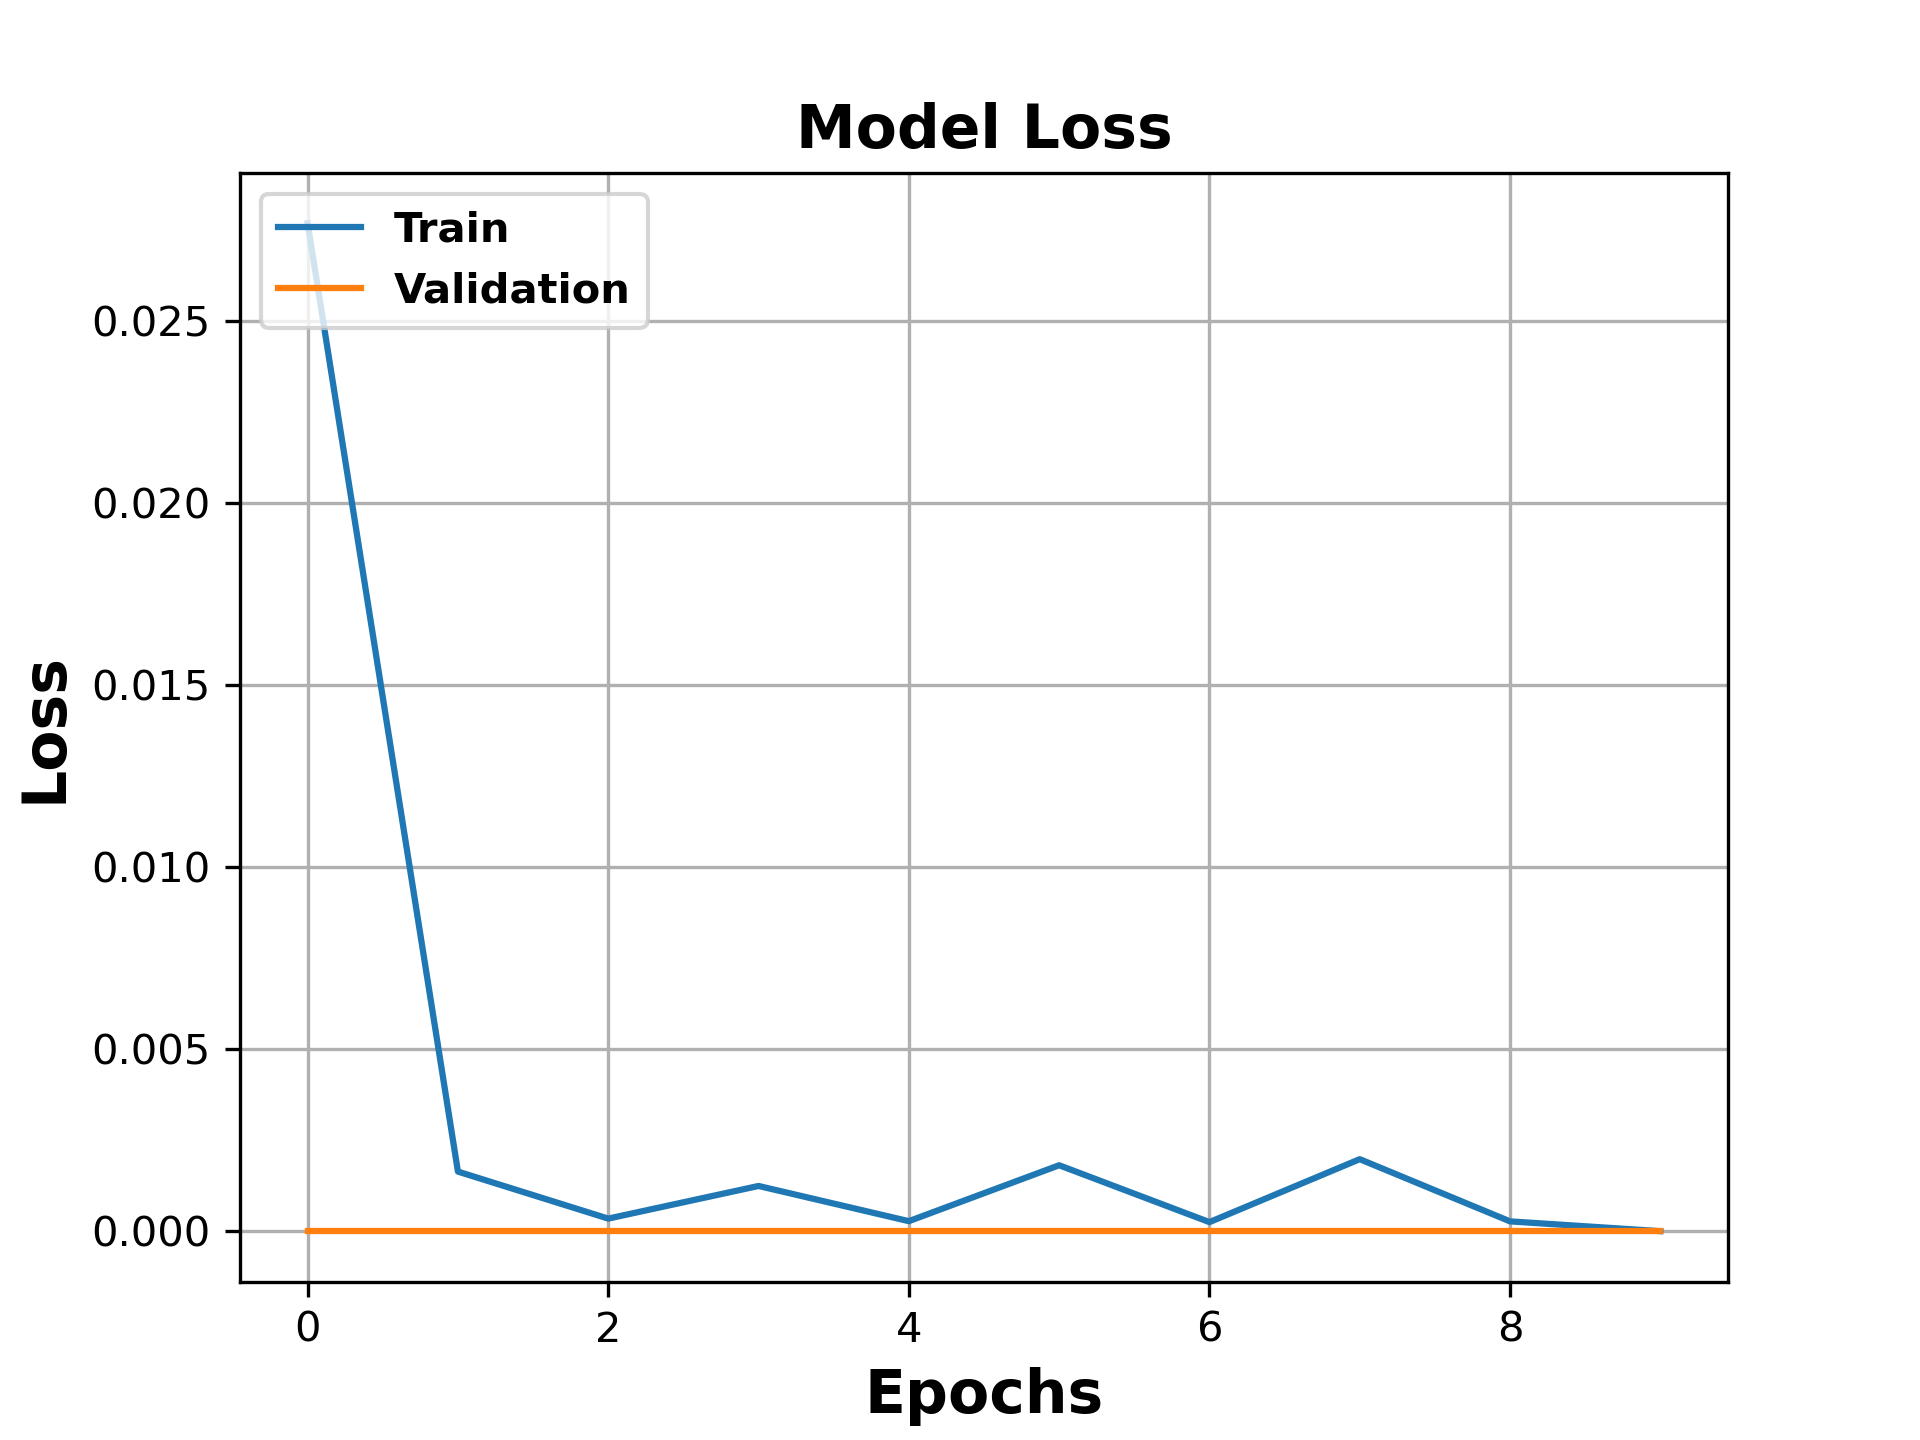
\includegraphics[width=\textwidth]{images/Evaluation/Synthetic_Data_Classifier_2021-05-31_16-40-33_Loss.png}
    \caption[Epochs vs. Loss plot during training a classifier on synthetic document images.]{Epochs vs. Loss plot during training a classifier on synthetic document images.}
    \label{fig:SyntheticClassifierLoss}
  \end{minipage}
\end{figure}

\begin{figure}[H]
    \begin{center}
	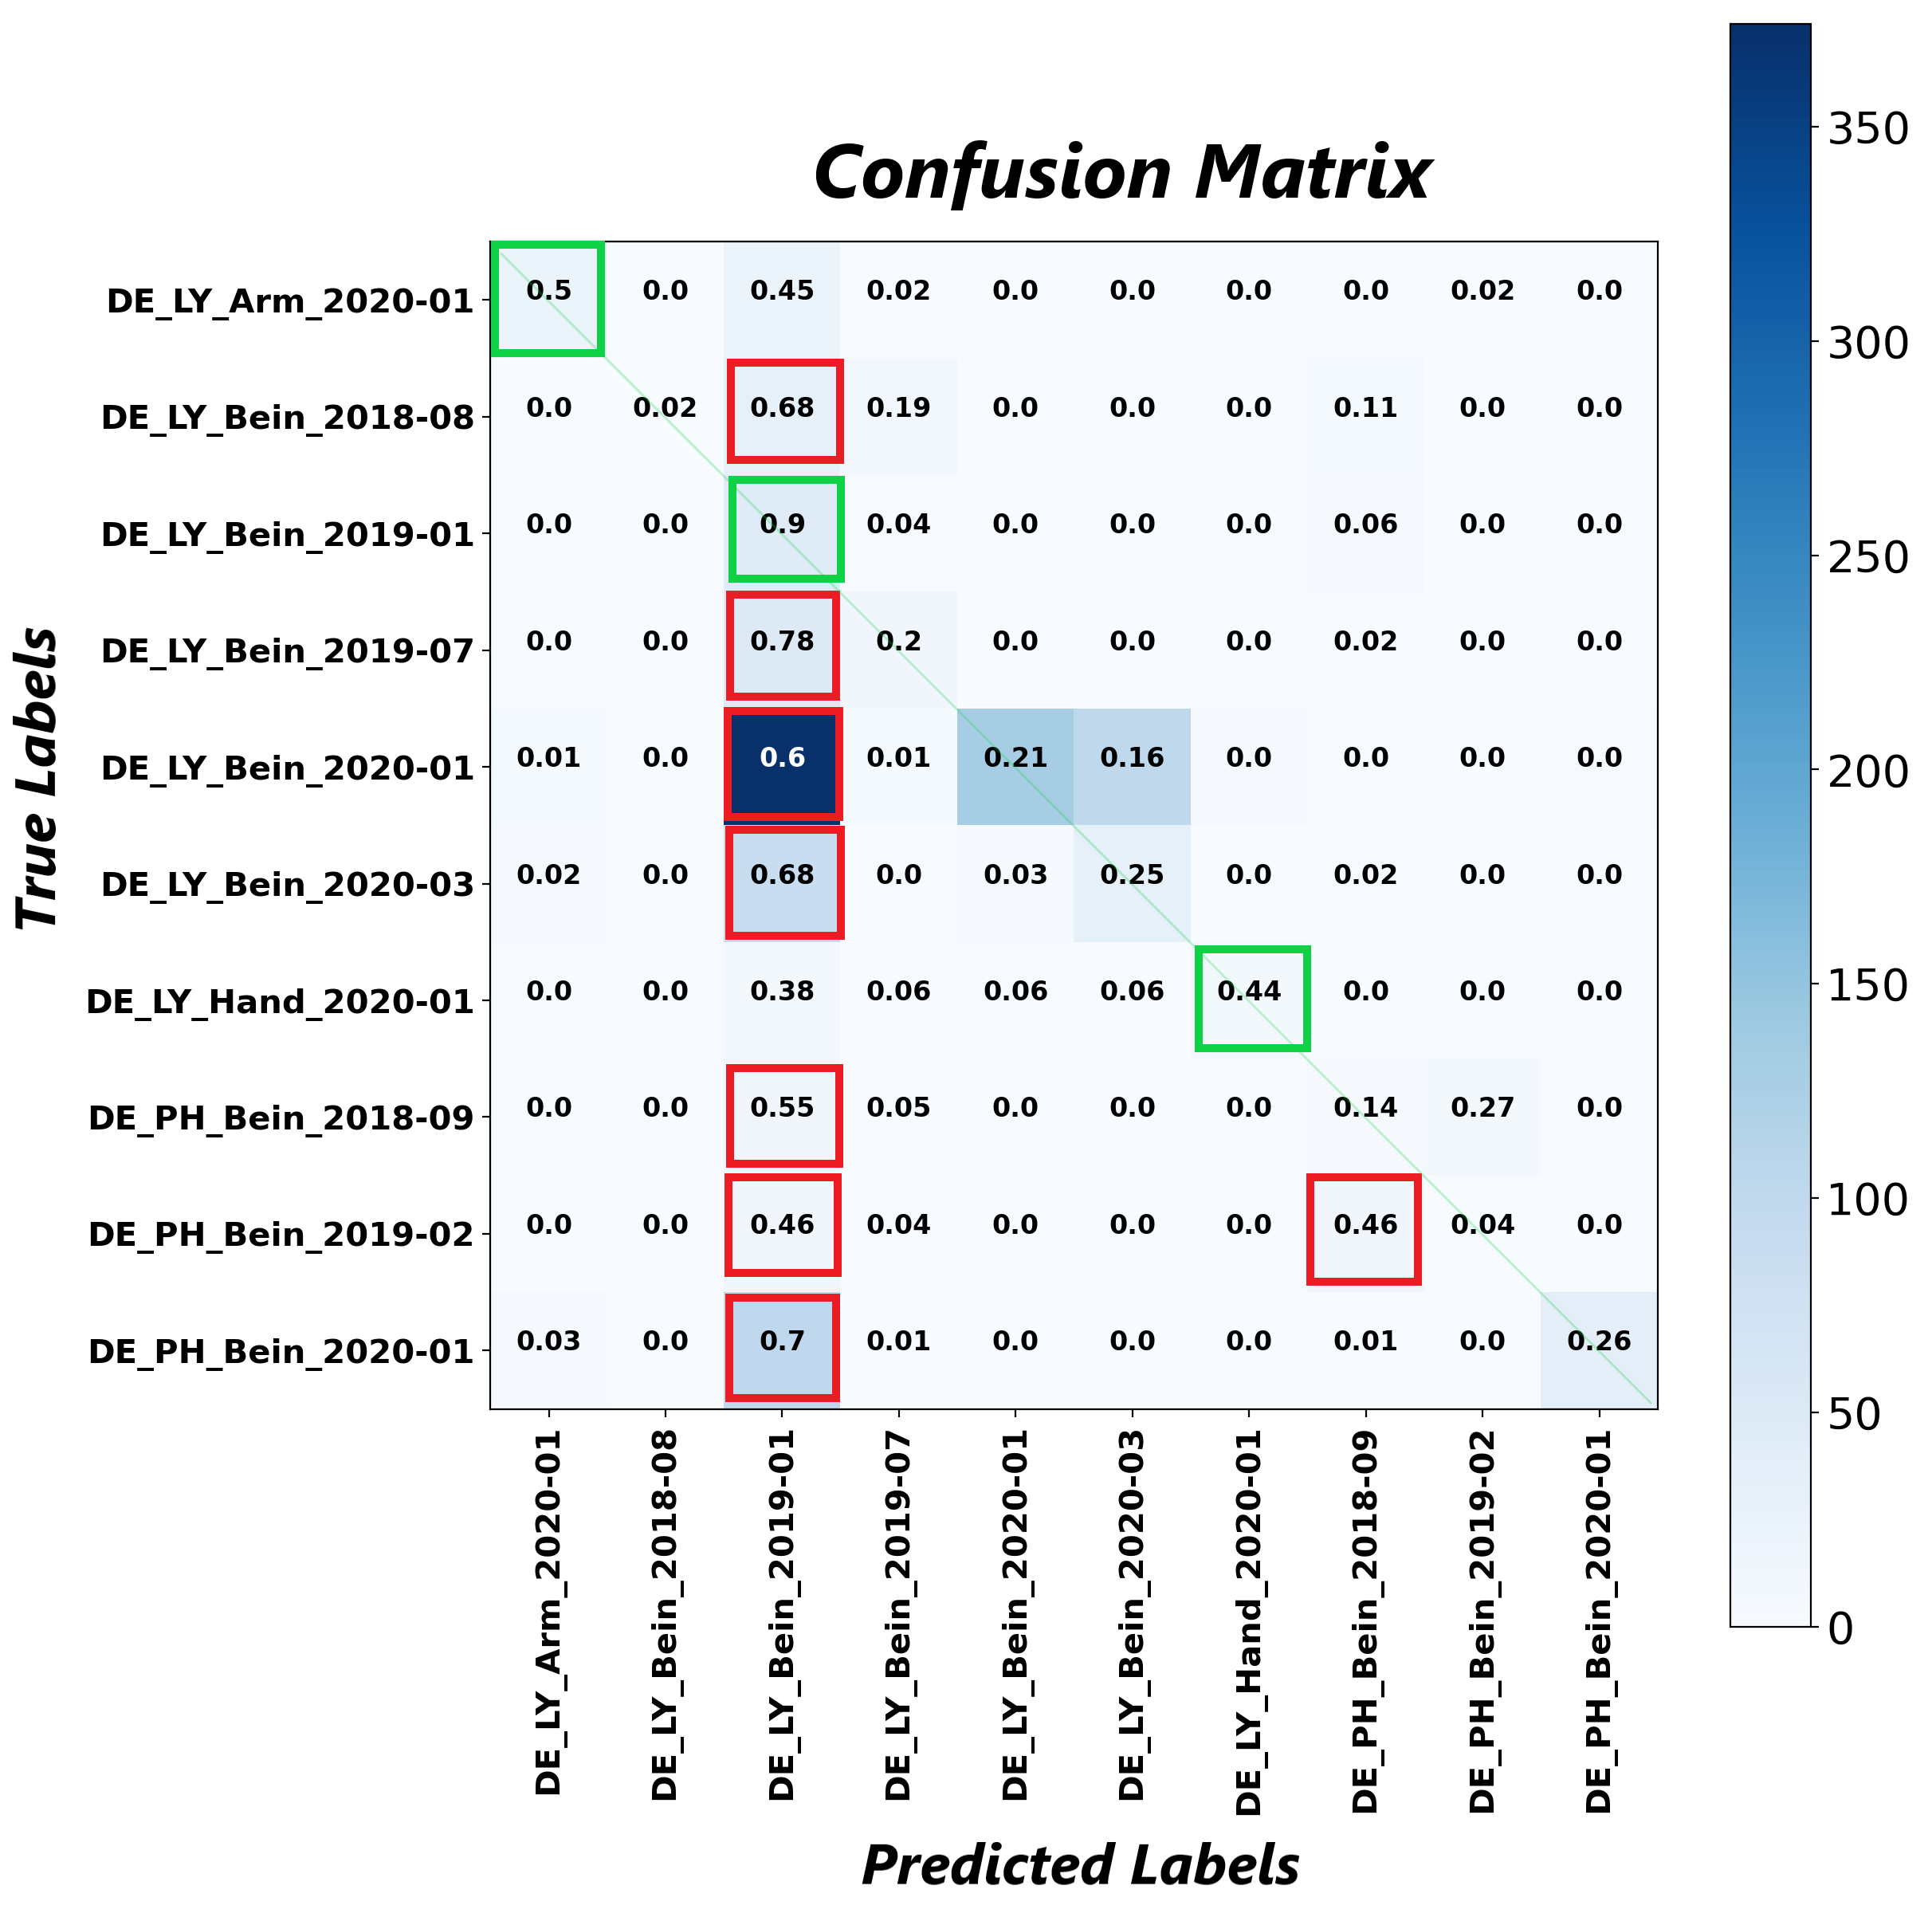
\includegraphics[scale=0.70]{images/Evaluation/Confusion_Matrix_Synthetic_Data_Classifier_2021-05-31_16-40-33.png}
	\caption[Confusion matrix to analyze the performance of the classifier trained on synthetic document images and evaluated using real annotated document images (test dataset).]{Confusion matrix to analyze the performance of the classifier trained on synthetic document images and evaluated using real annotated document images (test dataset).}
	\label{fig:CMSyntheticDocumentImagesClassifier}
	\end{center}
\end{figure}

\begin{center}
\begin{table}[H]
    \centering
    \begin{center}
    \begin{tabular}{P{0.22\linewidth} P{0.10\linewidth} P{0.10\linewidth} P{0.10\linewidth} P{0.10\linewidth}} 
        \toprule
            & Precision & Recall & F1-score & Support\\[0.0ex] 
        \midrule
        DE\_LY\_Arm\_2020-01 & 0.65 & 0.50 & 0.56 & 44\\[0.0ex]
        \midrule
        DE\_LY\_Bein\_2018-08 & 0.50 & 0.02 & 0.04 & 47\\[0.0ex]
        \midrule
        DE\_LY\_Bein\_2019-01 & 0.06 & 0.90 & 0.11 & 50\\[0.0ex]
        \midrule
        DE\_LY\_Bein\_2019-07 & 0.36 & 0.20 & 0.26 & 60\\[0.0ex]
        \midrule
        DE\_LY\_Bein\_2020-01 & 0.96 & 0.21 & 0.34 & 624\\[0.0ex]
        \midrule
        DE\_LY\_Bein\_2020-03 & 0.24 & 0.25 & 0.24 & 128\\[0.0ex]
        \midrule
        DE\_LY\_Hand\_2020-01 & 0.70 & 0.44 & 0.54 & 16\\[0.0ex]
        \midrule
        DE\_PH\_Bein\_2018-09 & 0.10 & 0.14 & 0.12 & 22\\[0.0ex]
        \midrule
        DE\_PH\_Bein\_2019-02 & 0.12 & 0.04 & 0.06 & 28\\[0.0ex]
        \midrule
        DE\_PH\_Bein\_2020-01 & 0.95 & 0.51 & 0.26 & 143\\[0.0ex]
        \midrule
        \midrule
        Accuracy              &      &      & \bf{0.25} & 1162\\[0.0ex]
        Macro average             & 0.46 & 0.29 &  \bf{0.27} & 1162\\[0.0ex]
        Weighted average          & 0.74 & 0.25 &  \bf{0.31} & 1162\\[0.0ex]
        \bottomrule
    \end{tabular}
    \caption[Classification report, evaluating a classifier on the testing dataset after training with synthetic document images.]{Classification report, evaluating a classifier on the testing dataset after training with synthetic document images.}
    \label{table:SyntheticClassificationReport}
    \end{center}
\end{table}
\end{center}



\subsection{Training a Classifier on Faxified Document Images}\label{trainingfaxifiedclassifier}


The faxification process mimics the way the fax machine works. Usually, the fax machines transmit only black-and-white images, but the transfered images might be dirty and not aligned perfectly. This leads to several common artifacts being introduced into transferred images. The faxification process attempts to mimic those introductions of artifacts into images. The faxification process transforms clean gray-scale synthetic document images in such a way like it was sent via fax. However, the faxification process is not deterministic, it involves randomness during the process of faxification of the images. It uses several image transformations like gamma transformation, brightness transformation, 180-degree rotations, resizing, rescaling, binarization, adding noise, adding verticle lines and conversion to a grayscale image. The faxification process can be visualized in figure \ref{fig:FaxificationProcess}. In figure \ref{fig:FaxificationProcessZoomed}, it is visible a snippet from the synthetic document image that has transformed into randomly distinct image transformations when it has sent through the faxification process. The faxification process is implemented in Python using a traditional programming approach.

The dataset of faxified document images is created by transforming synthetic document images using the faxification process (figure \ref{fig:FaxificationProcess}). In this experiment, the classifier is trained using the dataset of faxified document images. The performance of this classifier is evaluated on the testing dataset to understand the domain gap between real data distribution and faxified data distribution. The classification report in table \ref{table:FaxifiedClassificationReport} states that the accuracy of this classifier on testing dataset is 43\%, macro average F1-score is  58\% and weighted average F1-score is 43\%. The results conclude that the faxified data distribution matched the real data distribution better than the synthetic data distribution. The confusion matrix is illustrated in figure \ref{fig:CMFaxifiedDocumentImagesClassifier}. In which, it is visible that document images of class DE\_LY\_Bein\_2019-01 (support 50) are being wrongly classified as DE\_LY\_Bein\_2019-07. Also, the document images of class DE\_LY\_Bein\_2020-01 (support 624) are wrongly classified as DE\_LY\_Bein\_2020-03. The remaining images from the testing dataset are classified convincingly. The epochs against accuracy and epochs against loss plots while training classifier on faxified document images is illustrated in figure \ref{fig:FaxifiedClassifierAcc} and \ref{fig:FaxifiedClassifierLoss} respectively.



\vspace*{1cm}

\begin{figure}[H]
        \begin{center}
	    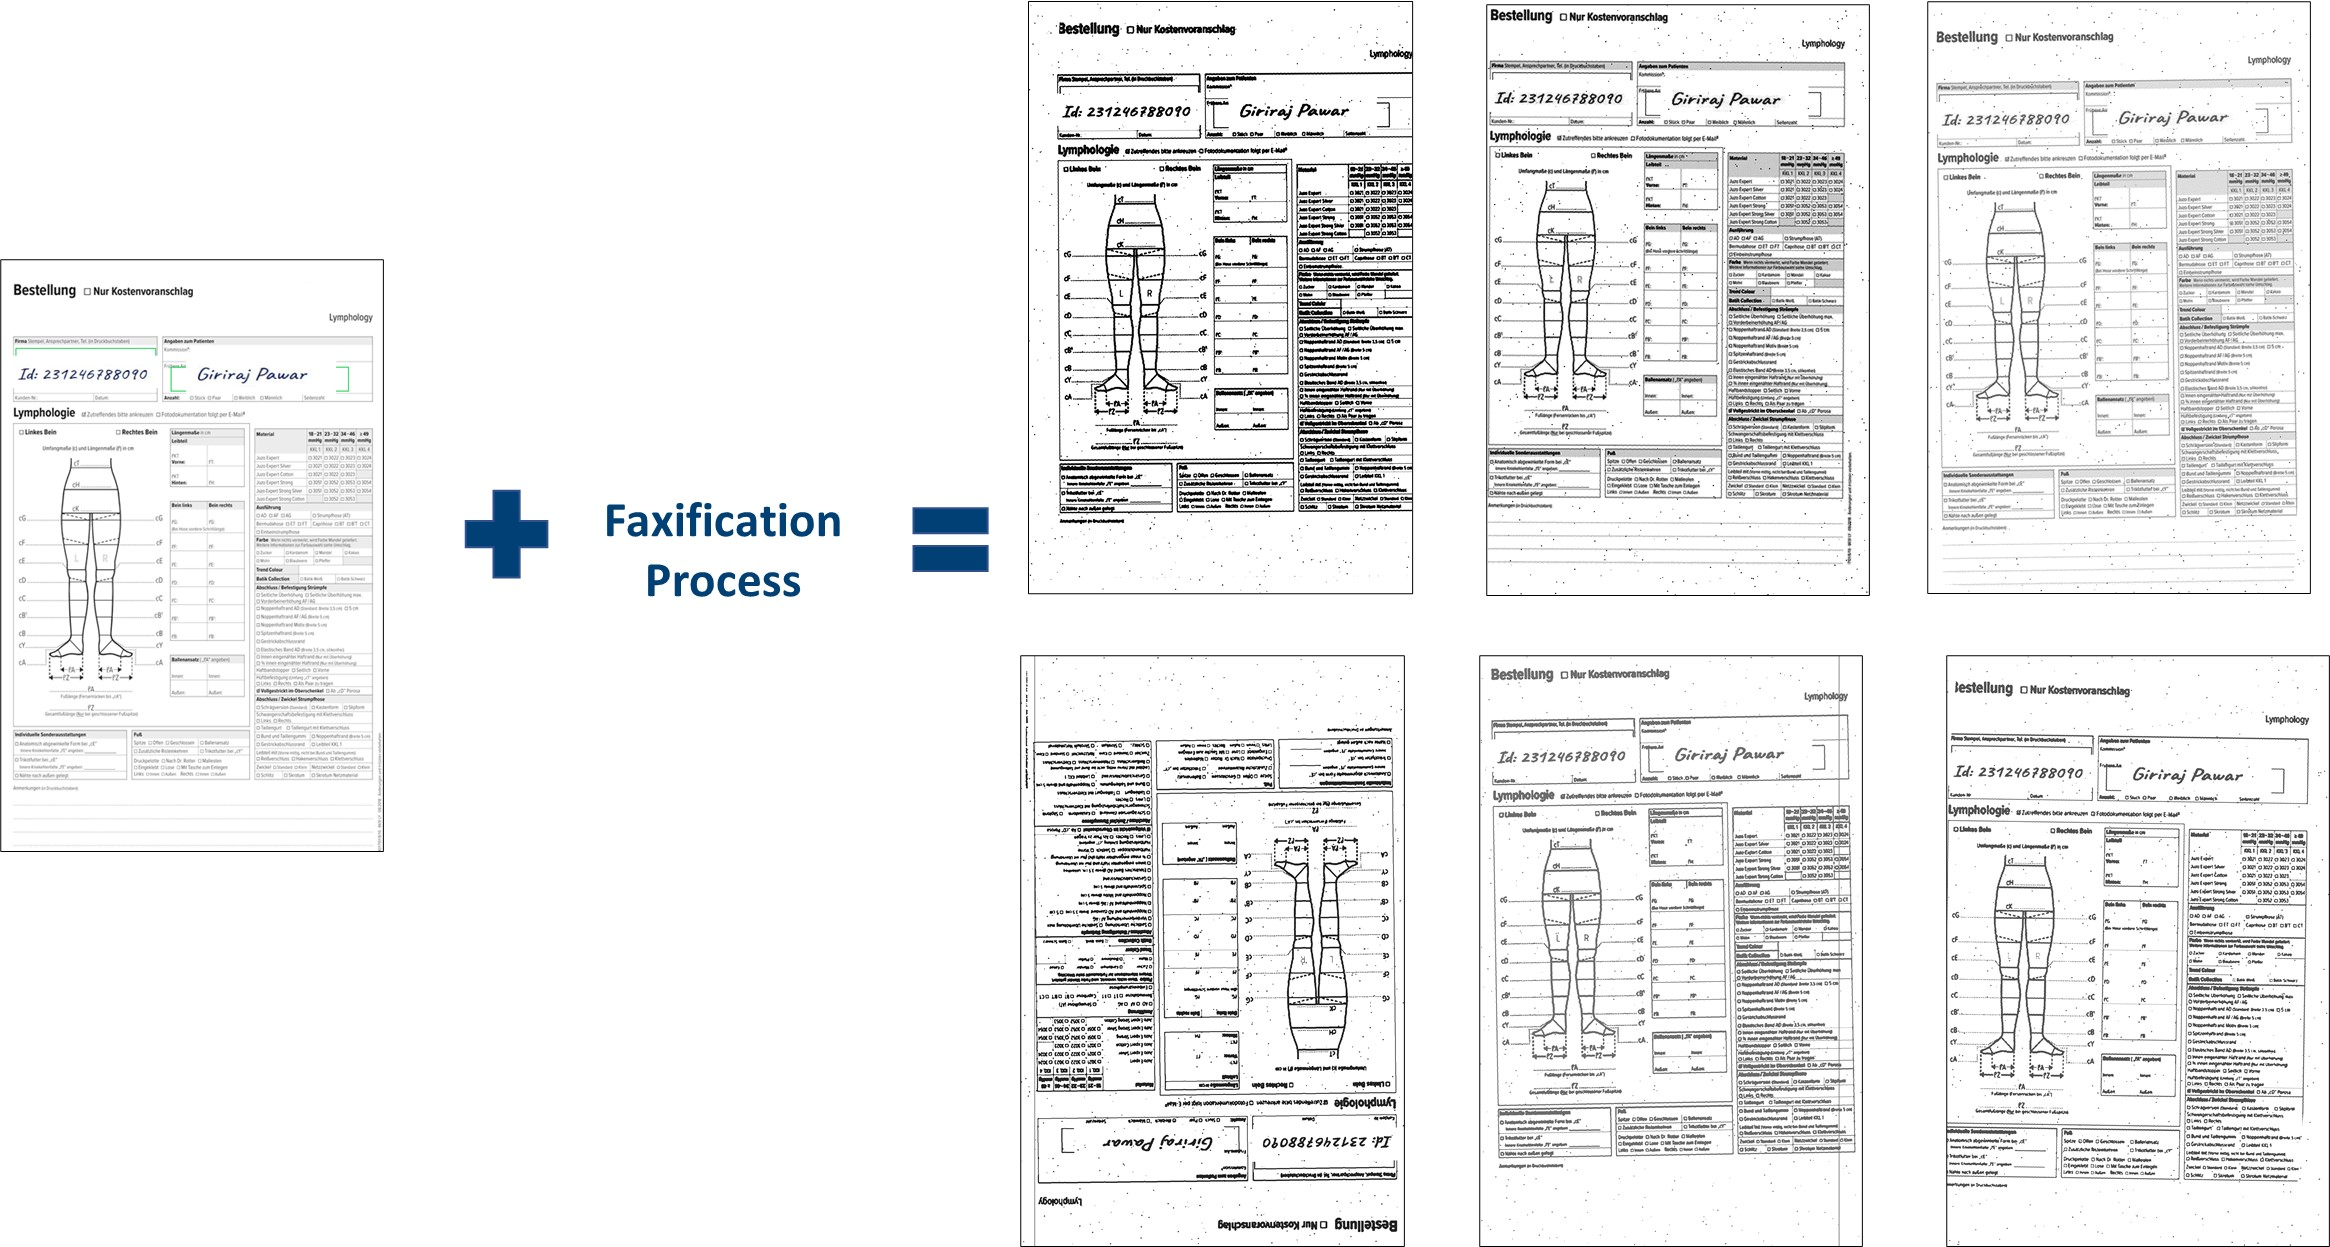
\includegraphics[scale=0.25]{images/Evaluation/FaxificationProcess.jpg}
	    \caption[An illustration of faxification process applied on synthetic document images.]{An illustration of faxification process applied on synthetic document images (figure reproduced from elevait GmbH \& Co. KG with permission).}
	    \label{fig:FaxificationProcess}
	    \end{center}
\end{figure}


\vspace*{2cm}
\begin{figure}[H]
        \begin{center}
	    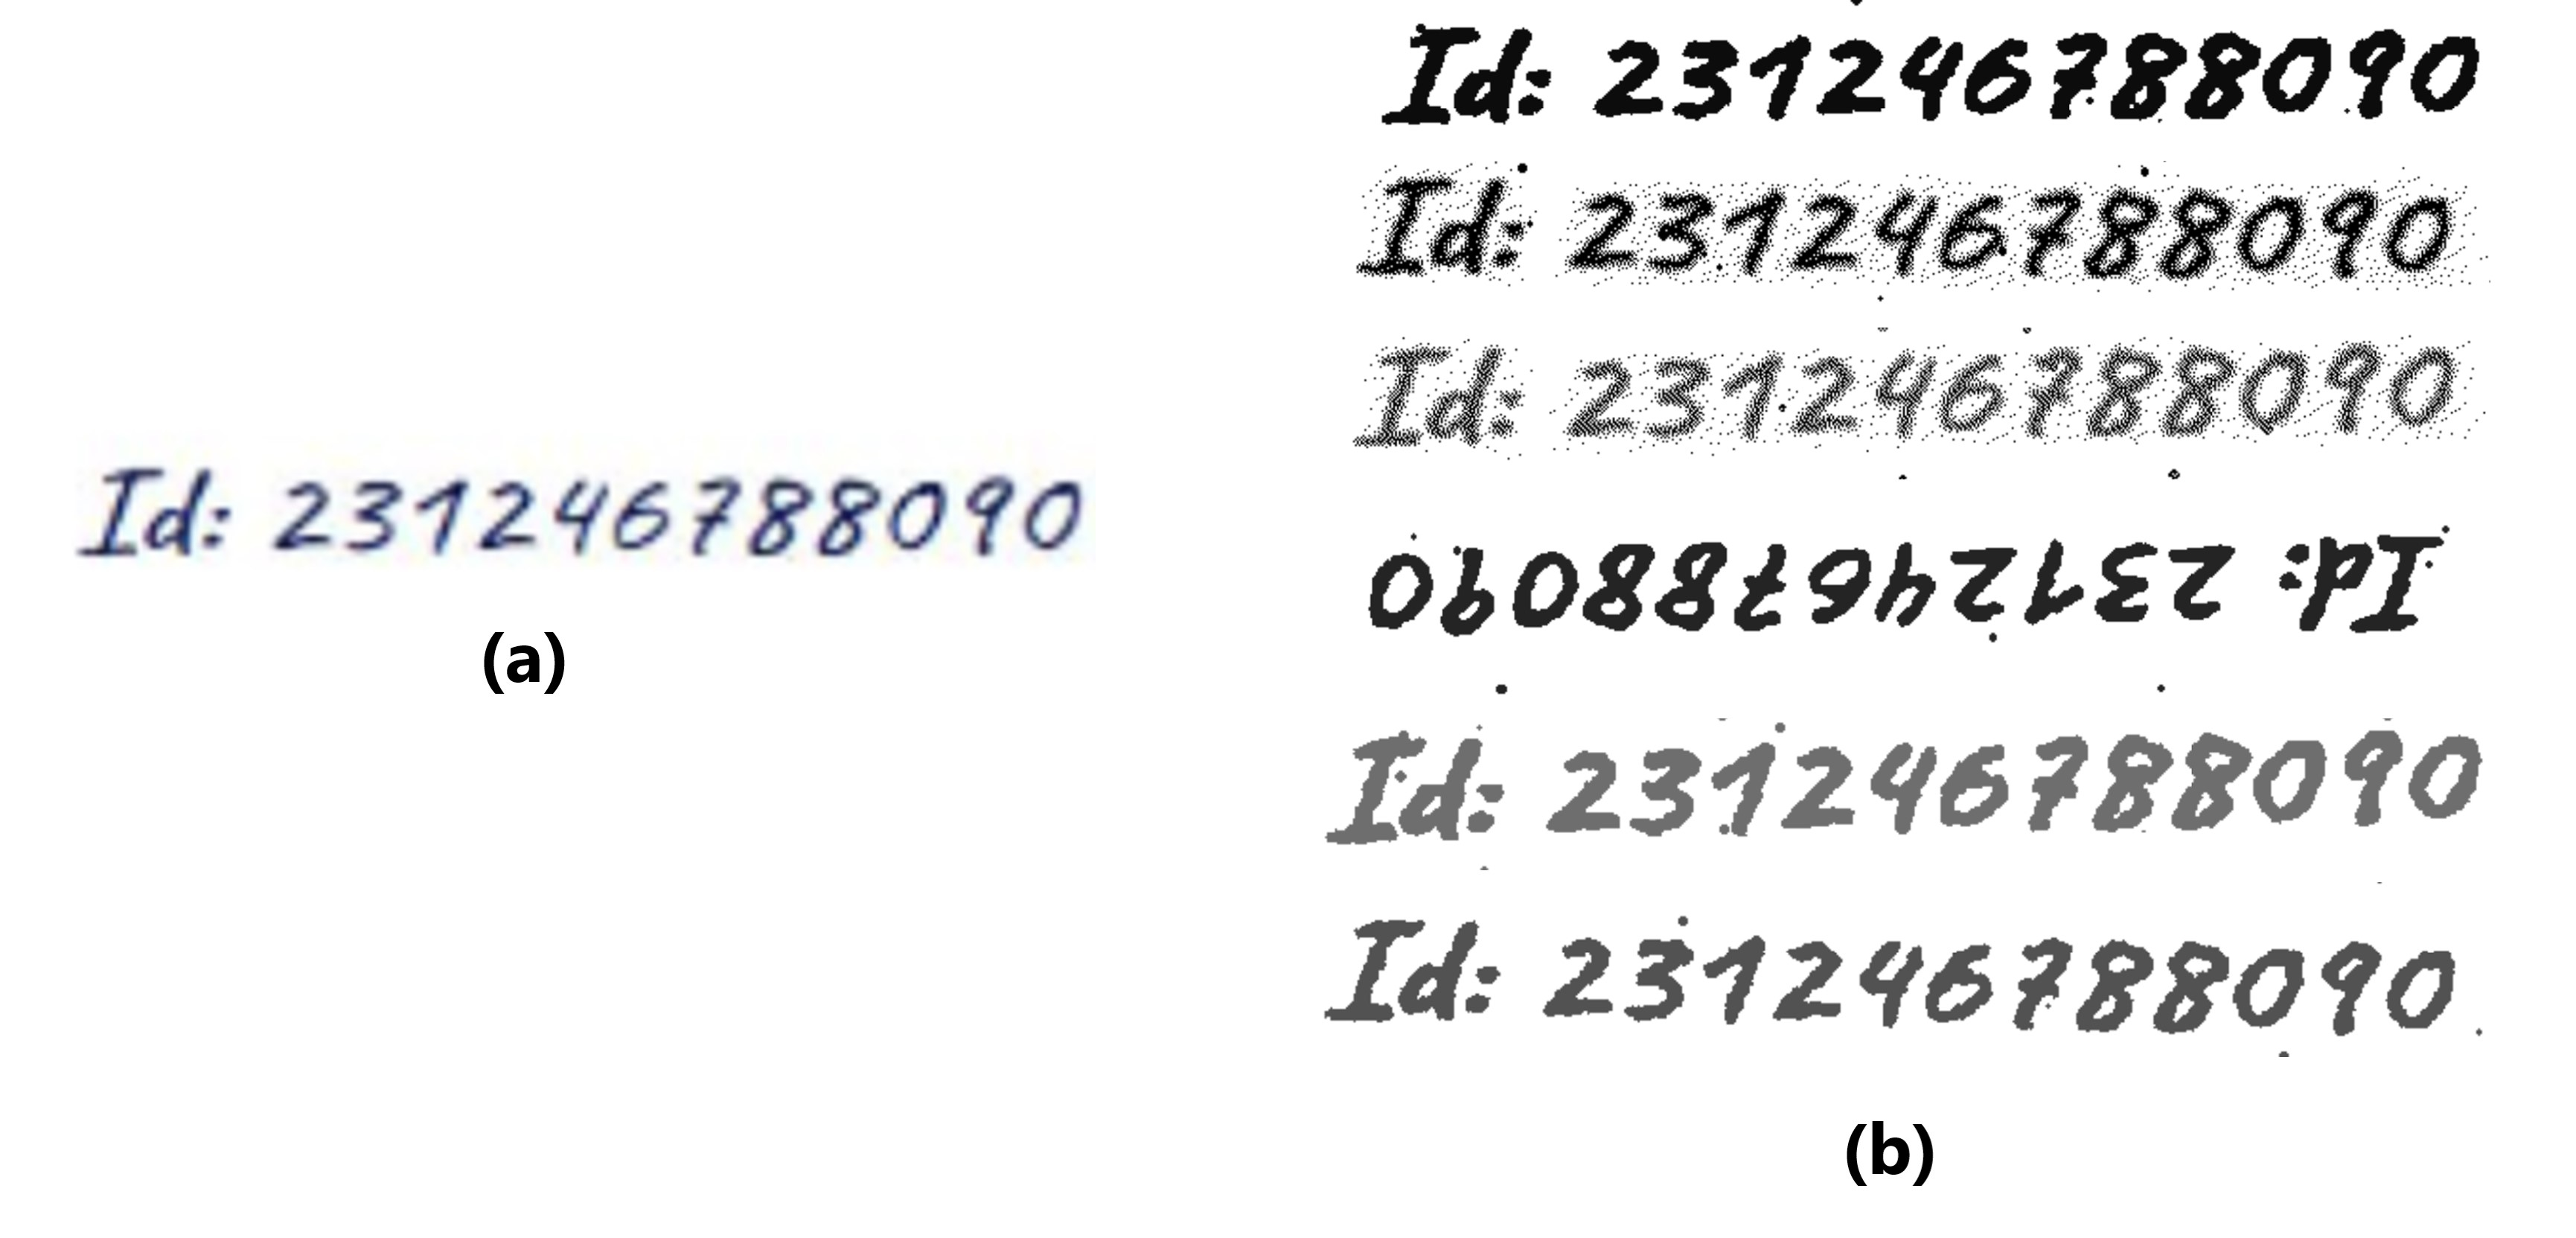
\includegraphics[scale=0.15]{images/Evaluation/FaxificationProcessZoomed.jpg}
	    \caption[An illustration of faxified document images to conclude that faxification process is a random process, the input images are faxified randomly to create distinct output.]{An illustration of faxified document images to conclude that faxification process is a random process, the input images are faxified randomly to create distinct and random output. For example, for a snippet in a synthetic document image (a), snippets of faxified document images shown in (b) are created distinct and random.}
	    \label{fig:FaxificationProcessZoomed}
	    \end{center}
\end{figure}


\vspace*{2cm}
\begin{figure}[H]
  \centering
  \begin{minipage}[b]{0.49\textwidth}
    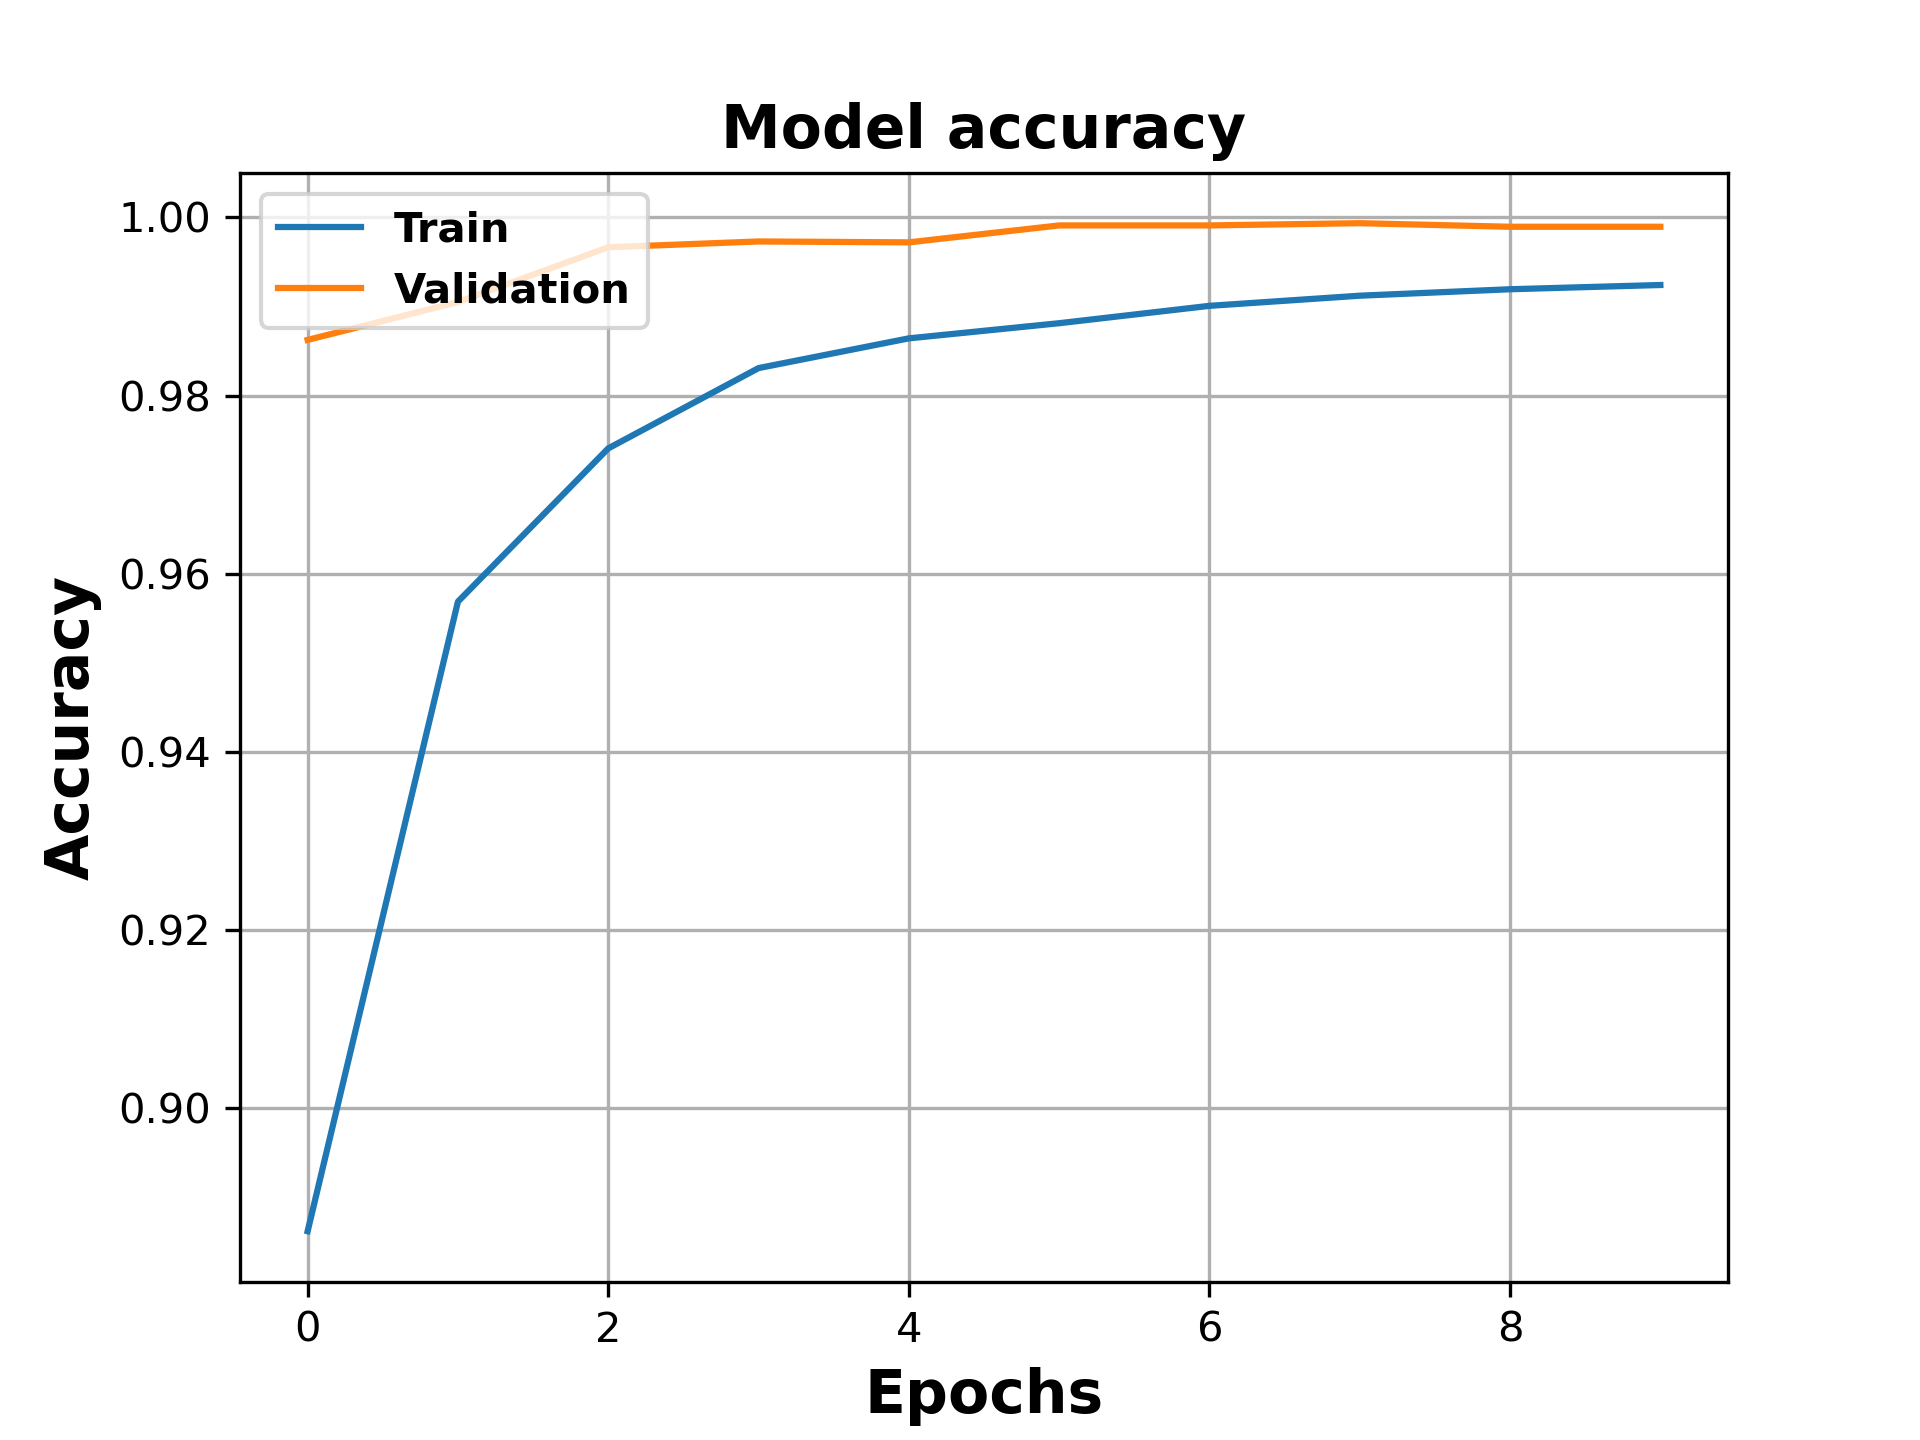
\includegraphics[width=\textwidth]{images/Evaluation/Faxified_Data_Classifier_2021-05-31_19-31-35_Accuracy.png}
    \caption[Epoch vs. Accuracy plot during training a classifier on faxified document images.]{Epoch vs. Accuracy plot during training a classifier on  faxified document images.}
    \label{fig:FaxifiedClassifierAcc}
  \end{minipage}
  \hfill
  \begin{minipage}[b]{0.49\textwidth}
    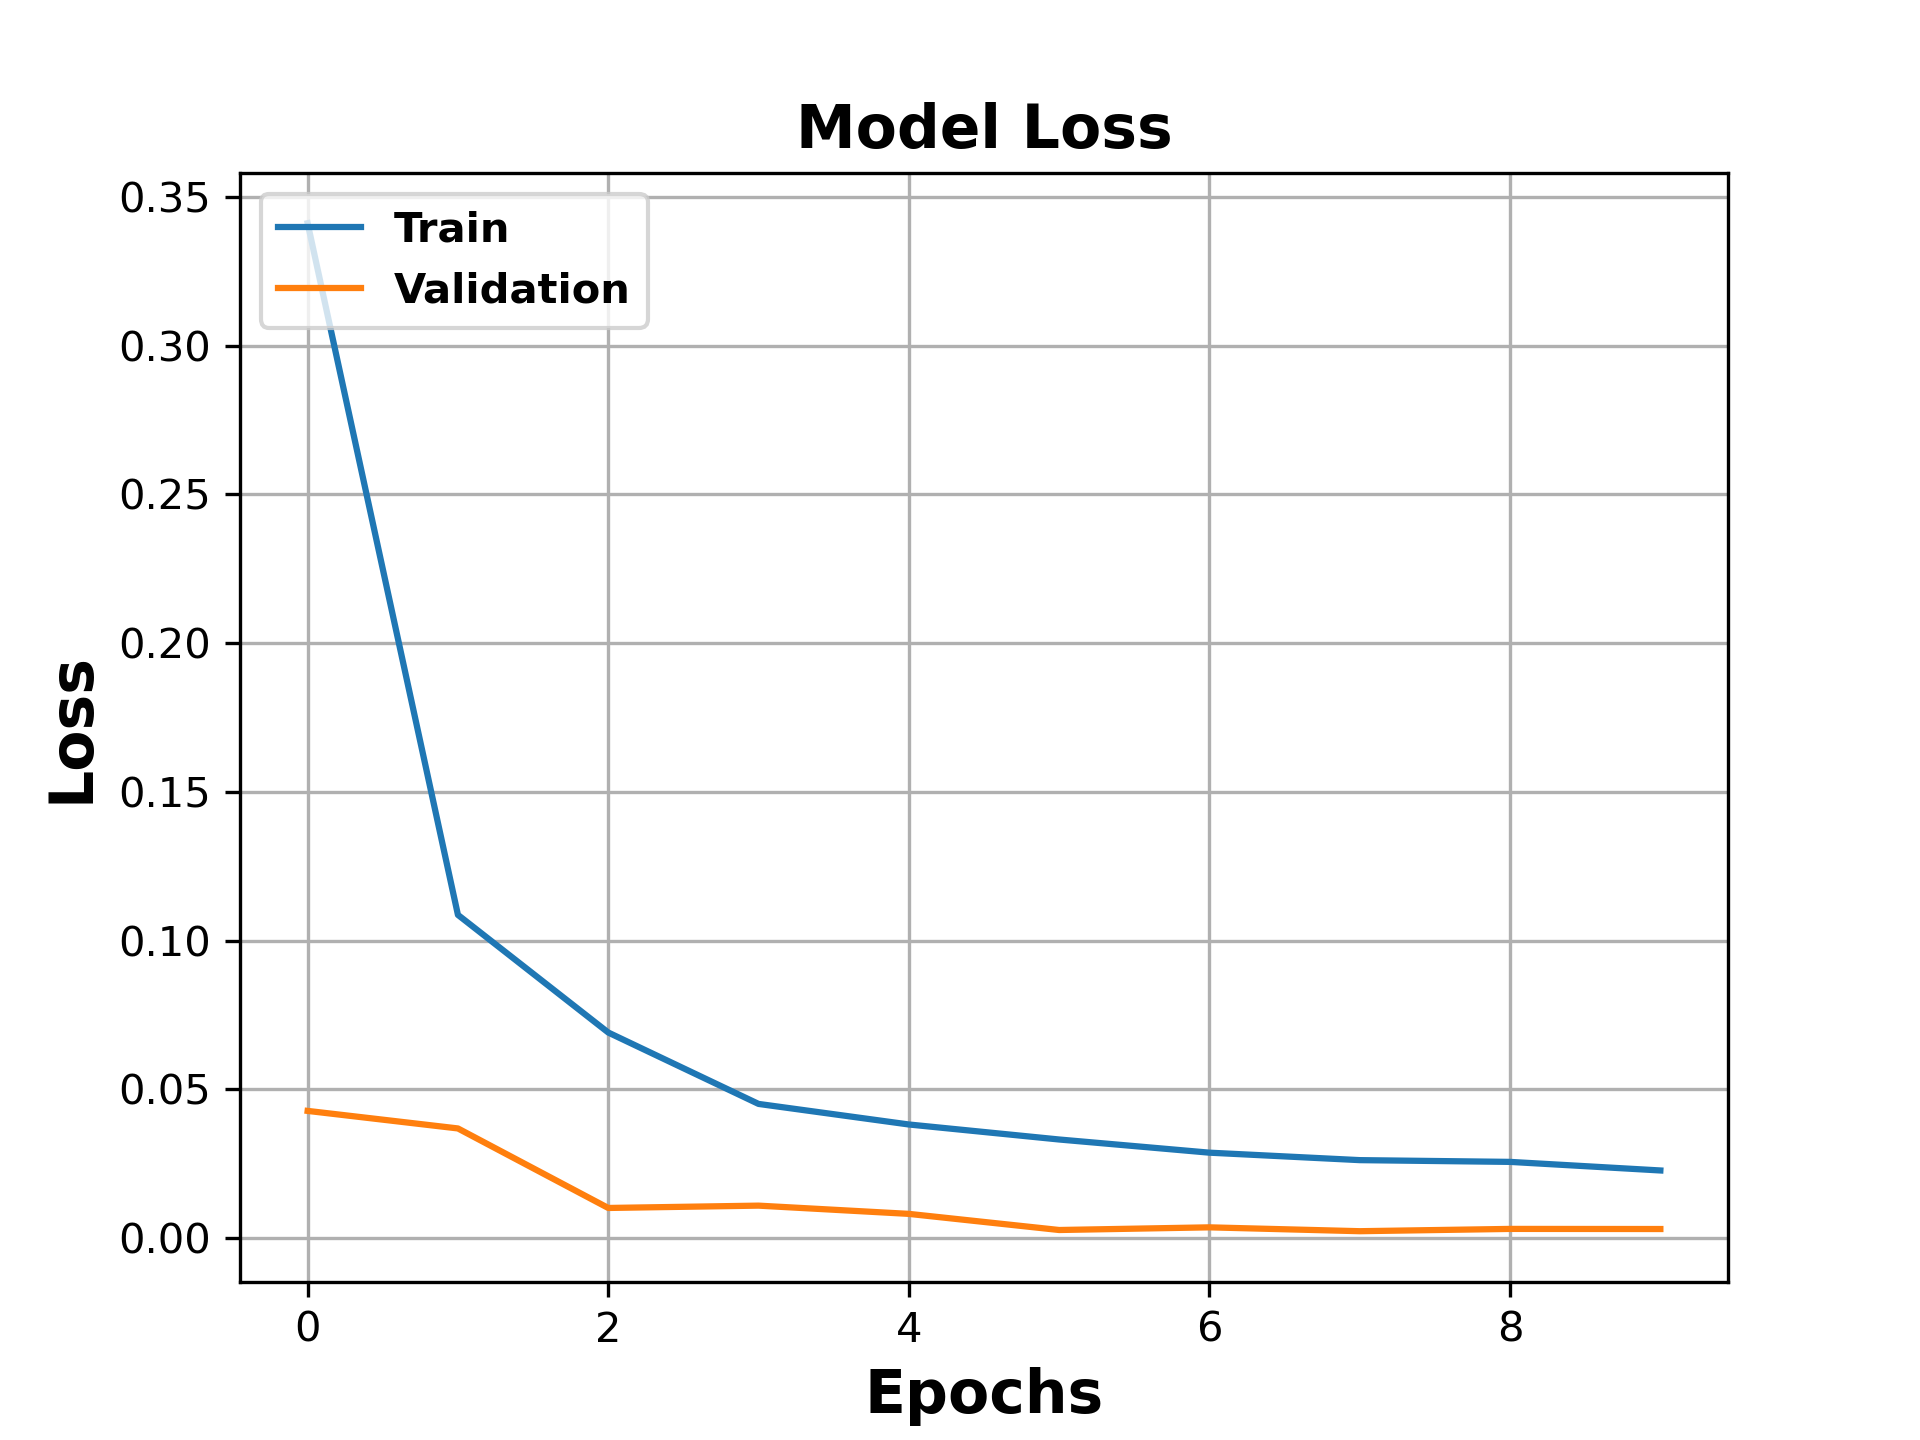
\includegraphics[width=\textwidth]{images/Evaluation/Faxified_Data_Classifier_2021-05-31_19-31-35_Loss.png}
    \caption[Epoch vs. Loss plot during training a classifier on faxified document images.]{Epoch vs. Loss plot during training a classifier on faxified document images.}
    \label{fig:FaxifiedClassifierLoss}
  \end{minipage}
\end{figure}






%Also, compared to other data distributions like synthetic and \ac{CycleGAN} generated, the faxified data distribution is more similar to the real data distribution. 


\begin{figure}[H]
    \begin{center}
	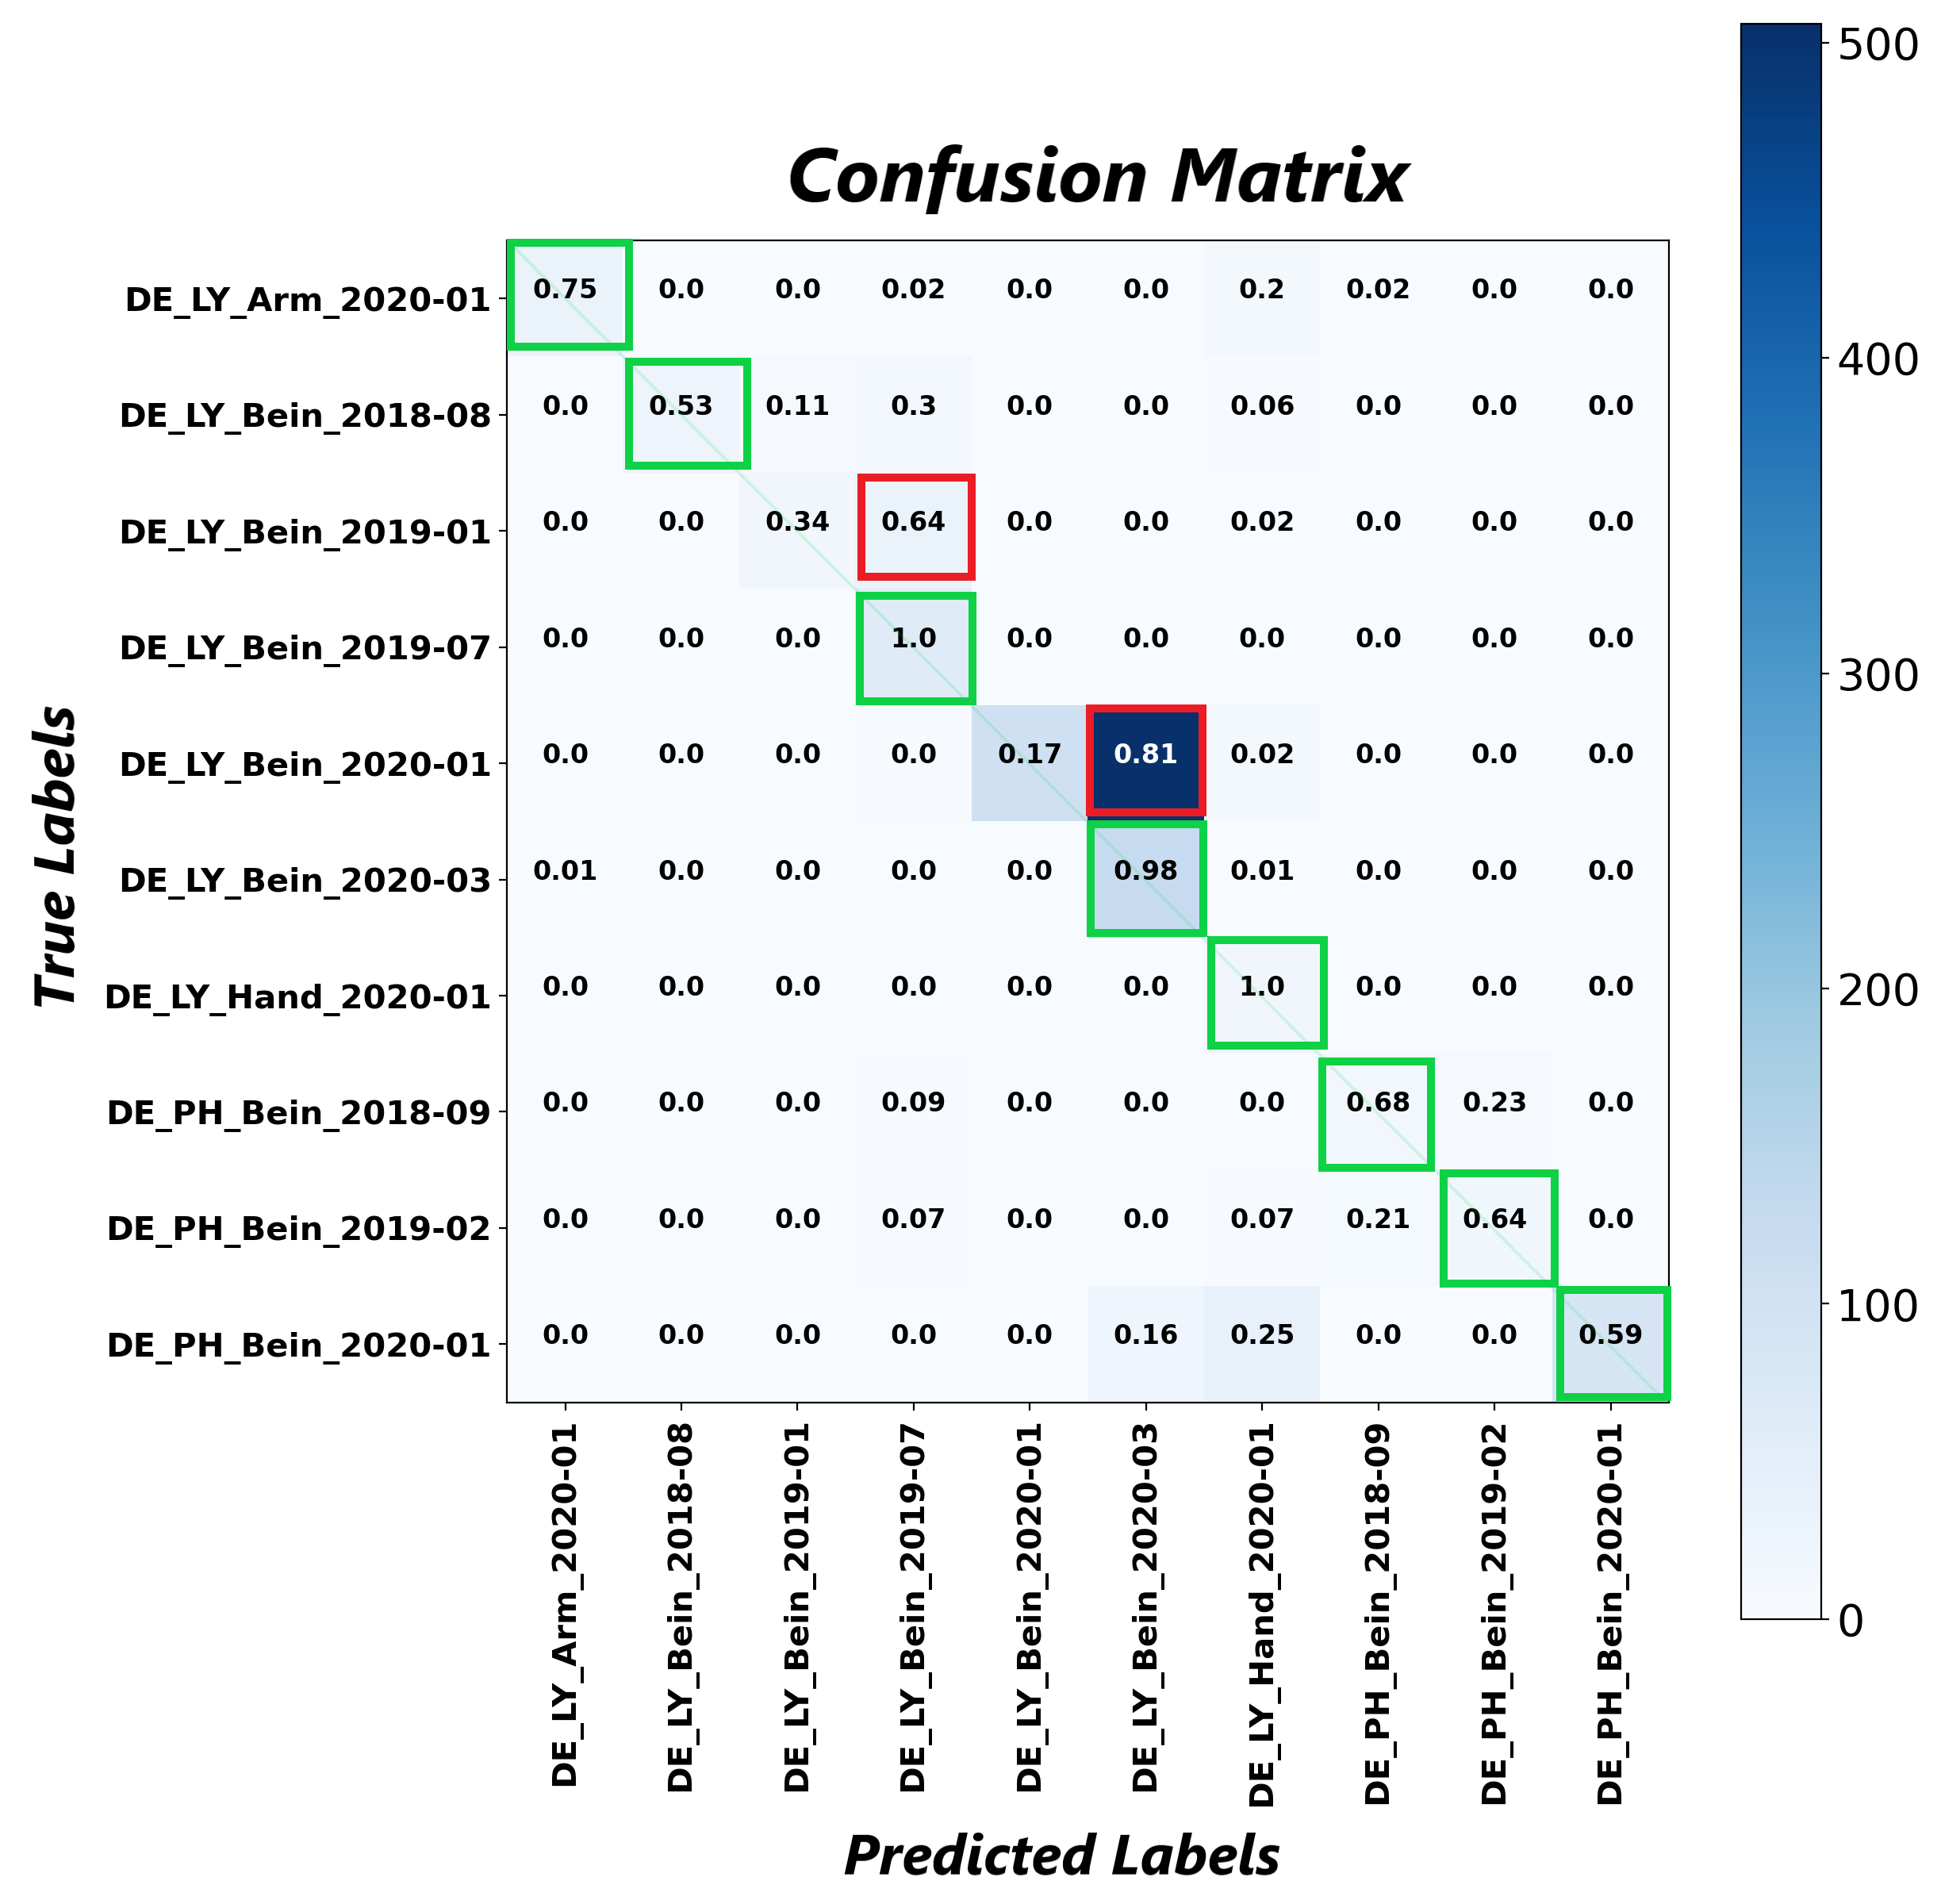
\includegraphics[scale=0.70]{images/Evaluation/Confusion_Matrix_Faxified_Data_Classifier_2021-05-31_19-31-35.png}
	\caption[Confusion matrix to analyze the performance of the classifier trained on faxified document images and evaluated using real annotated document images (test dataset).]{Confusion matrix to analyze the performance of the classifier trained on faxified document images and evaluated using real annotated document images (test dataset).}
	\label{fig:CMFaxifiedDocumentImagesClassifier}
	\end{center}
\end{figure}

\begin{center}
\begin{table}[H]
    \begin{center}
    \begin{tabular}{P{0.22\linewidth} P{0.10\linewidth} P{0.10\linewidth} P{0.10\linewidth} P{0.10\linewidth}} 
        \toprule
            & Precision & Recall & F1-score & Support\\[0.0ex] 
        \midrule
        DE\_LY\_Arm\_2020-01 & 0.97 & 0.75 & 0.85 & 44\\[0.0ex]
        \midrule
        DE\_LY\_Bein\_2018-08 & 1.00 & 0.53 & 0.69 & 47\\[0.0ex]
        \midrule
        DE\_LY\_Bein\_2019-01 & 0.74 & 0.34 & 0.47 & 50\\[0.0ex]
        \midrule
        DE\_LY\_Bein\_2019-07 & 0.53 & 1.00 & 0.69 & 60\\[0.0ex]
        \midrule
        DE\_LY\_Bein\_2020-01 & 1.00 & 0.17 & 0.29 & 624\\[0.0ex]
        \midrule
        DE\_LY\_Bein\_2020-03 & 0.19 & 0.98 & 0.32 & 128\\[0.0ex]
        \midrule
        DE\_LY\_Hand\_2020-01 & 0.21 & 1.00 & 0.34 & 16\\[0.0ex]
        \midrule
        DE\_PH\_Bein\_2018-09 & 0.68 & 0.68 & 0.68 & 22\\[0.0ex]
        \midrule
        DE\_PH\_Bein\_2019-02 & 0.78 & 0.64 & 0.71 & 28\\[0.0ex]
        \midrule
        DE\_PH\_Bein\_2020-01 & 1.00 & 0.59 & 0.74 & 143\\[0.0ex]
        \midrule
        \midrule
        Accuracy              &      &      & \bf{0.43} & 1162\\[0.0ex]
        Macro average             & 0.71 & 0.67 & \bf{0.58} & 1162\\[0.0ex]
        Weighted average          & 0.85 & 0.43 & \bf{0.43} & 1162\\[0.0ex]

        \bottomrule
    \end{tabular}
    \caption[Classification report, evaluating a classifier on the testing dataset after training with faxified document images.]{Classification report, evaluating a classifier on the testing dataset after training with faxified document images.}
    \label{table:FaxifiedClassificationReport}
    \end{center}
\end{table}
\end{center}



\subsection{\ac{CycleGAN} Training}


%The proposed image-to-image translation application is implemented using \ac{CycleGAN}. It is trained for 20 epochs and with batch size 1. The \ac{CycleGAN} consists of two generators $G$ and $F$ and two discriminators $D_X$ and $D_Y$. The domain $X$ represents the source domain and domain $Y$ represents the target domain. The developed image-to-image translation application aims to transform synthetic document images into realistic document images. Hence, the synthetic document images represent the source domain and real document images represent the target domain. The complete architecture of the proposed image-to-image translation application using \ac{CycleGAN} is illustrated in figure \ref{fig:GxyFyx}. For more \ac{CycleGAN} training details refer section \ref{TrainingDetailsCycleGAN}. 

%The \ac{CycleGAN} training happens by calculating loss and updating the weights of discriminators $D_X$ and $D_Y$ and generators $G$ and $F$ respectively. 




The proposed image-to-image translation application is implemented using \ac{CycleGAN}. The \ac{CycleGAN} is trained using synthetic document images (Domain $X$) and real document images (Domain $Y$). The domain $X$ represents the source domain and domain $Y$ represents the target domain. The \ac{CycleGAN} consists of two generators $G$ and $F$ and two discriminators $D_X$ and $D_Y$. Further, for training, random input images $x_i$ and $y_i$ are retrieved from source domain $X$ and target domain $Y$. The fake image generated using generator $G$ is $Generated\_Y$ and the fake image generated using generator by $F$ is $Generated\_X$. As we described earlier, $G$ is a mapping function to transform an image from source domain $X$ to target domain $Y$, mathematically it is $G: X \rightarrow Y$ and $F$ is vice versa $F: Y \rightarrow X$. The generator $G$ is called the forward generator and $F$ is called the backward generator. The discriminator loss for $D_X$ and $D_Y$ on real and fake images is computed. The computed discriminator loss is used to update the weights of respective discriminator. Next, the cycle-consistency loss is calculated by transforming the source domain image into the target domain, back again into the source domain. It is called forward cycle-consistency loss. It is calculated by determining the difference between the original image in the source domain and cycled image back in the source domain. Please refer to figure \ref{fig:GxyFyx}, the forward cycle-consistency loss is the difference between \textit{Input\_X} and \textit{Cyclic\_X}. The backward cycle-consistency loss is calculated by transforming the target domain image into the source domain, back again into the target domain. In figure \ref{fig:GxyFyx}, the backward cycle-consistency loss is the difference between \textit{Input\_Y} and \textit{Cyclic\_Y}. The cycle-consistency loss forces generating an image that is context instead of generating random images.


\begin{figure}[H]
  \centering
  \begin{minipage}[b]{0.49\textwidth}
    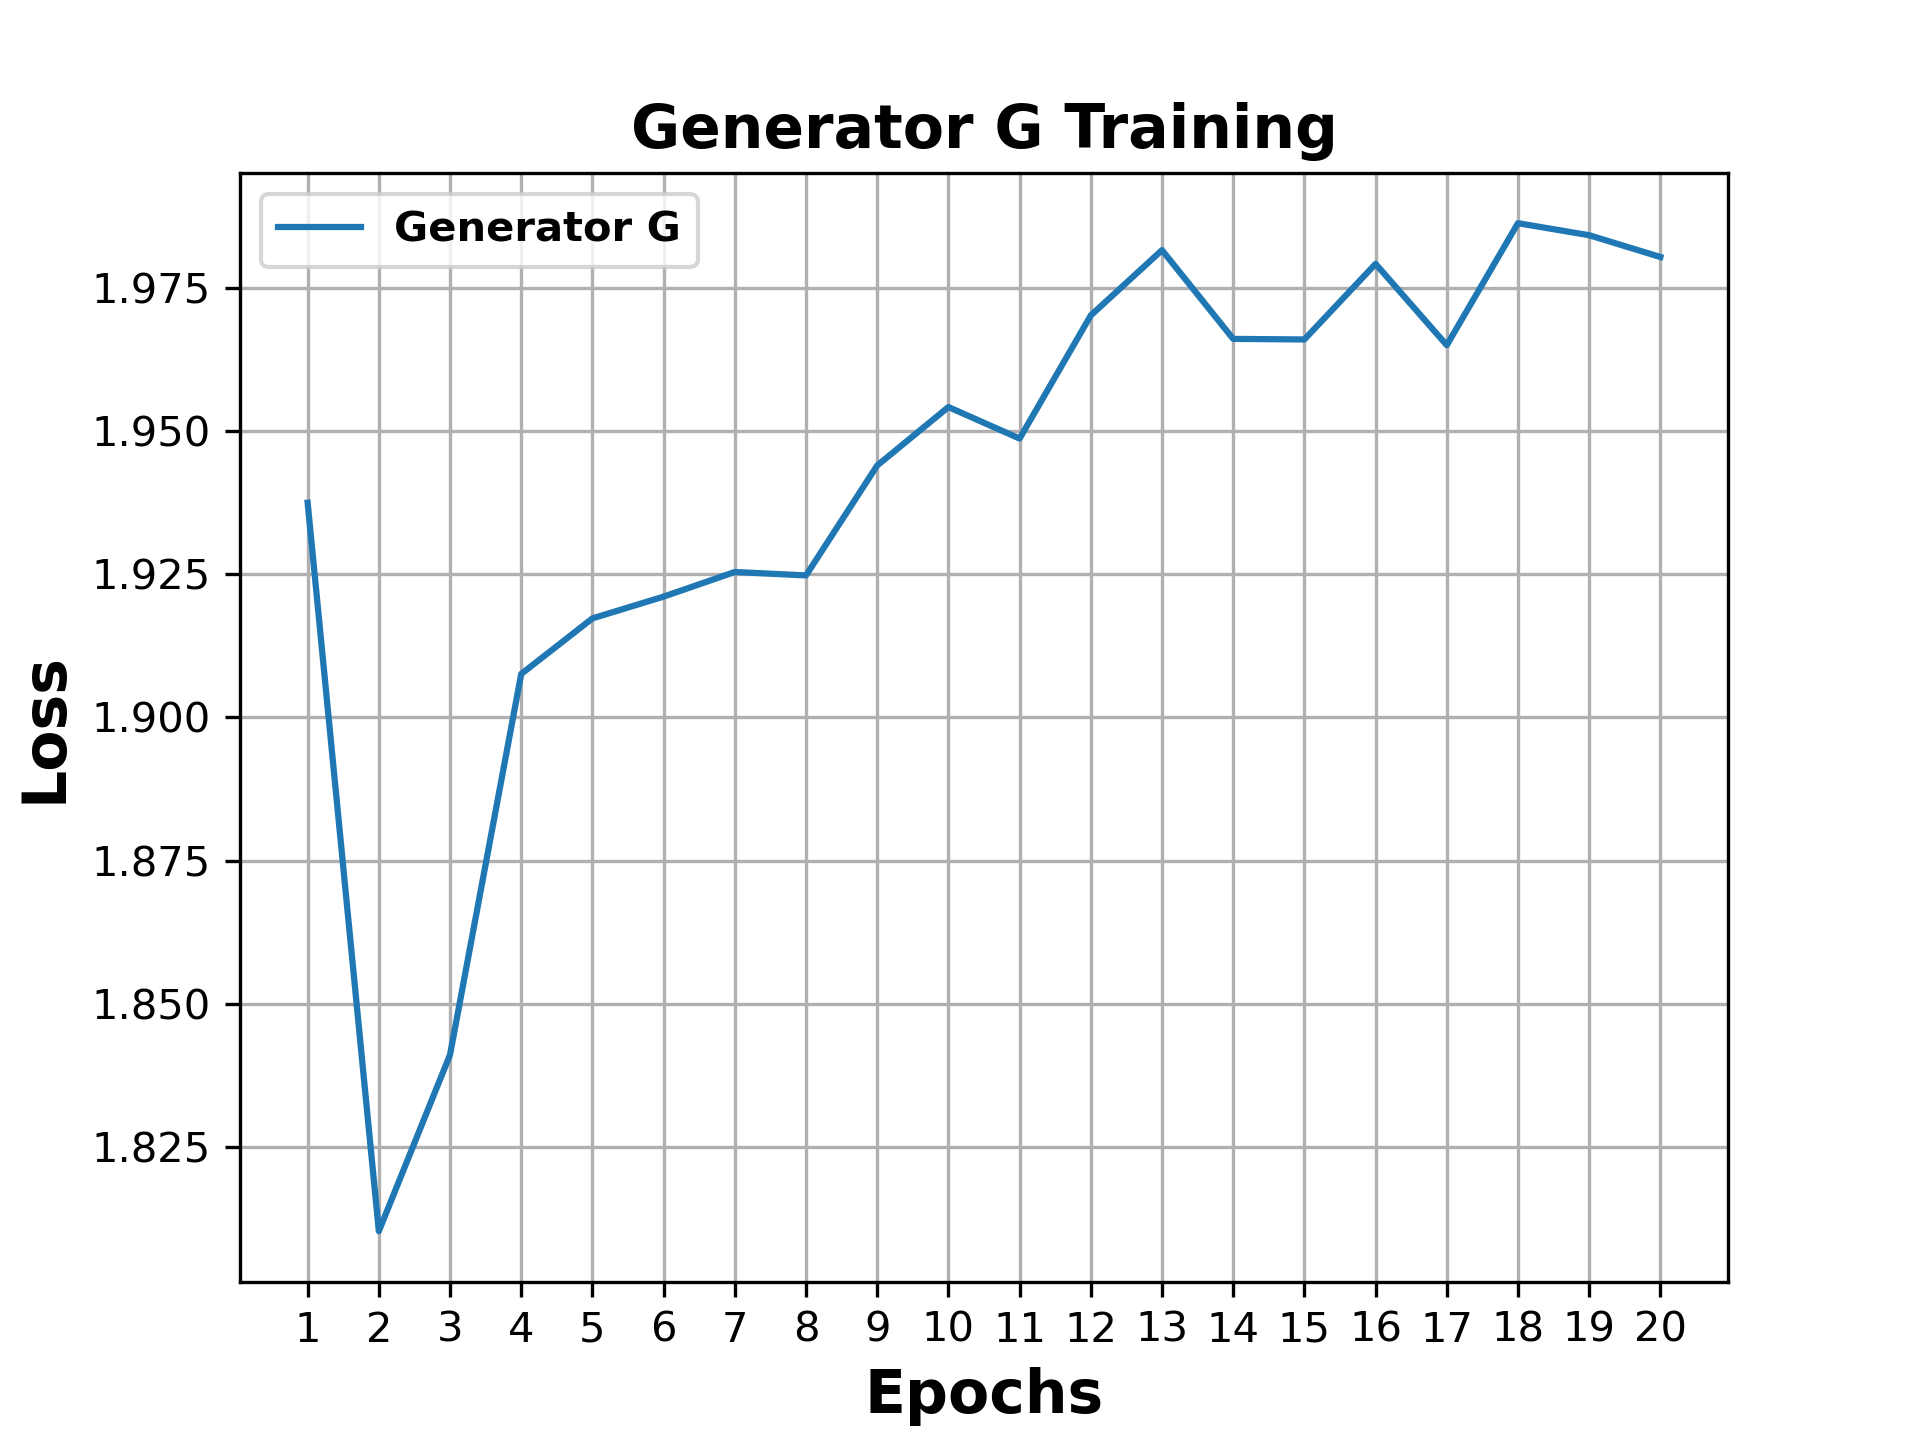
\includegraphics[width=\textwidth]{images/Evaluation/GeneratorGTraining.png}
    \caption[Epochs vs. Loss plot during Generator $G$ is training.]{Epochs vs. Loss plot during Generator $G$ is training.}
    \label{fig:generatorG}
  \end{minipage}
  \hfill
  \begin{minipage}[b]{0.49\textwidth}
    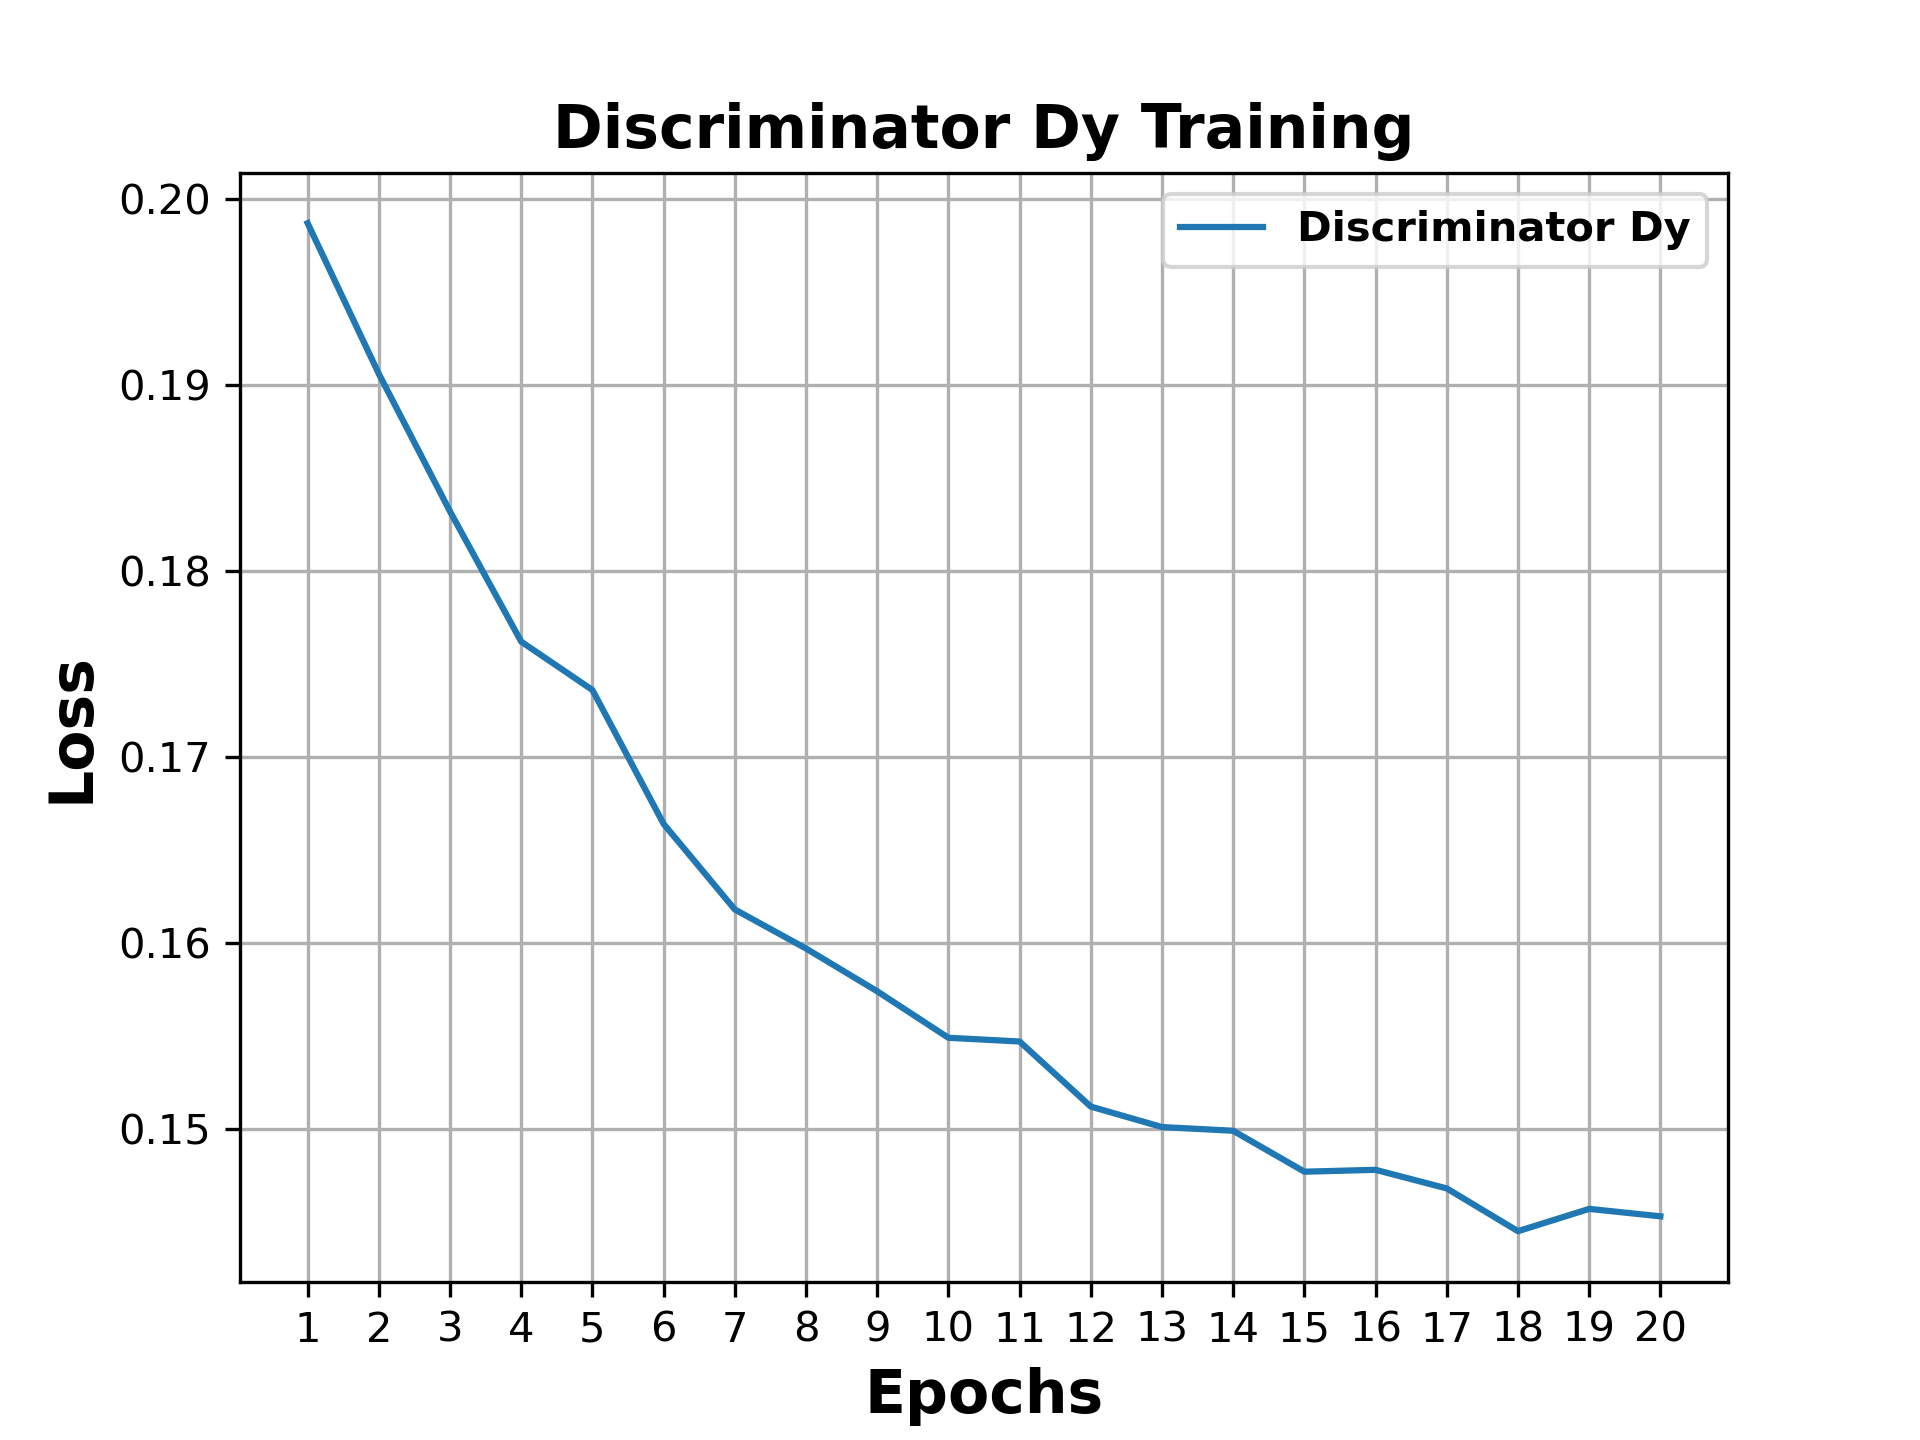
\includegraphics[width=\textwidth]{images/Evaluation/DiscriminatorDyTraining.png}
    \caption[Epochs vs. Loss plot during Discriminator $D_Y$ is training.]{Epochs vs. Loss plot during Discriminator $D_Y$ is training.}
    \label{fig:discriminatorDy}
  \end{minipage}
\end{figure}

\begin{figure}[H]
  \centering
  \begin{minipage}[b]{0.49\textwidth}
    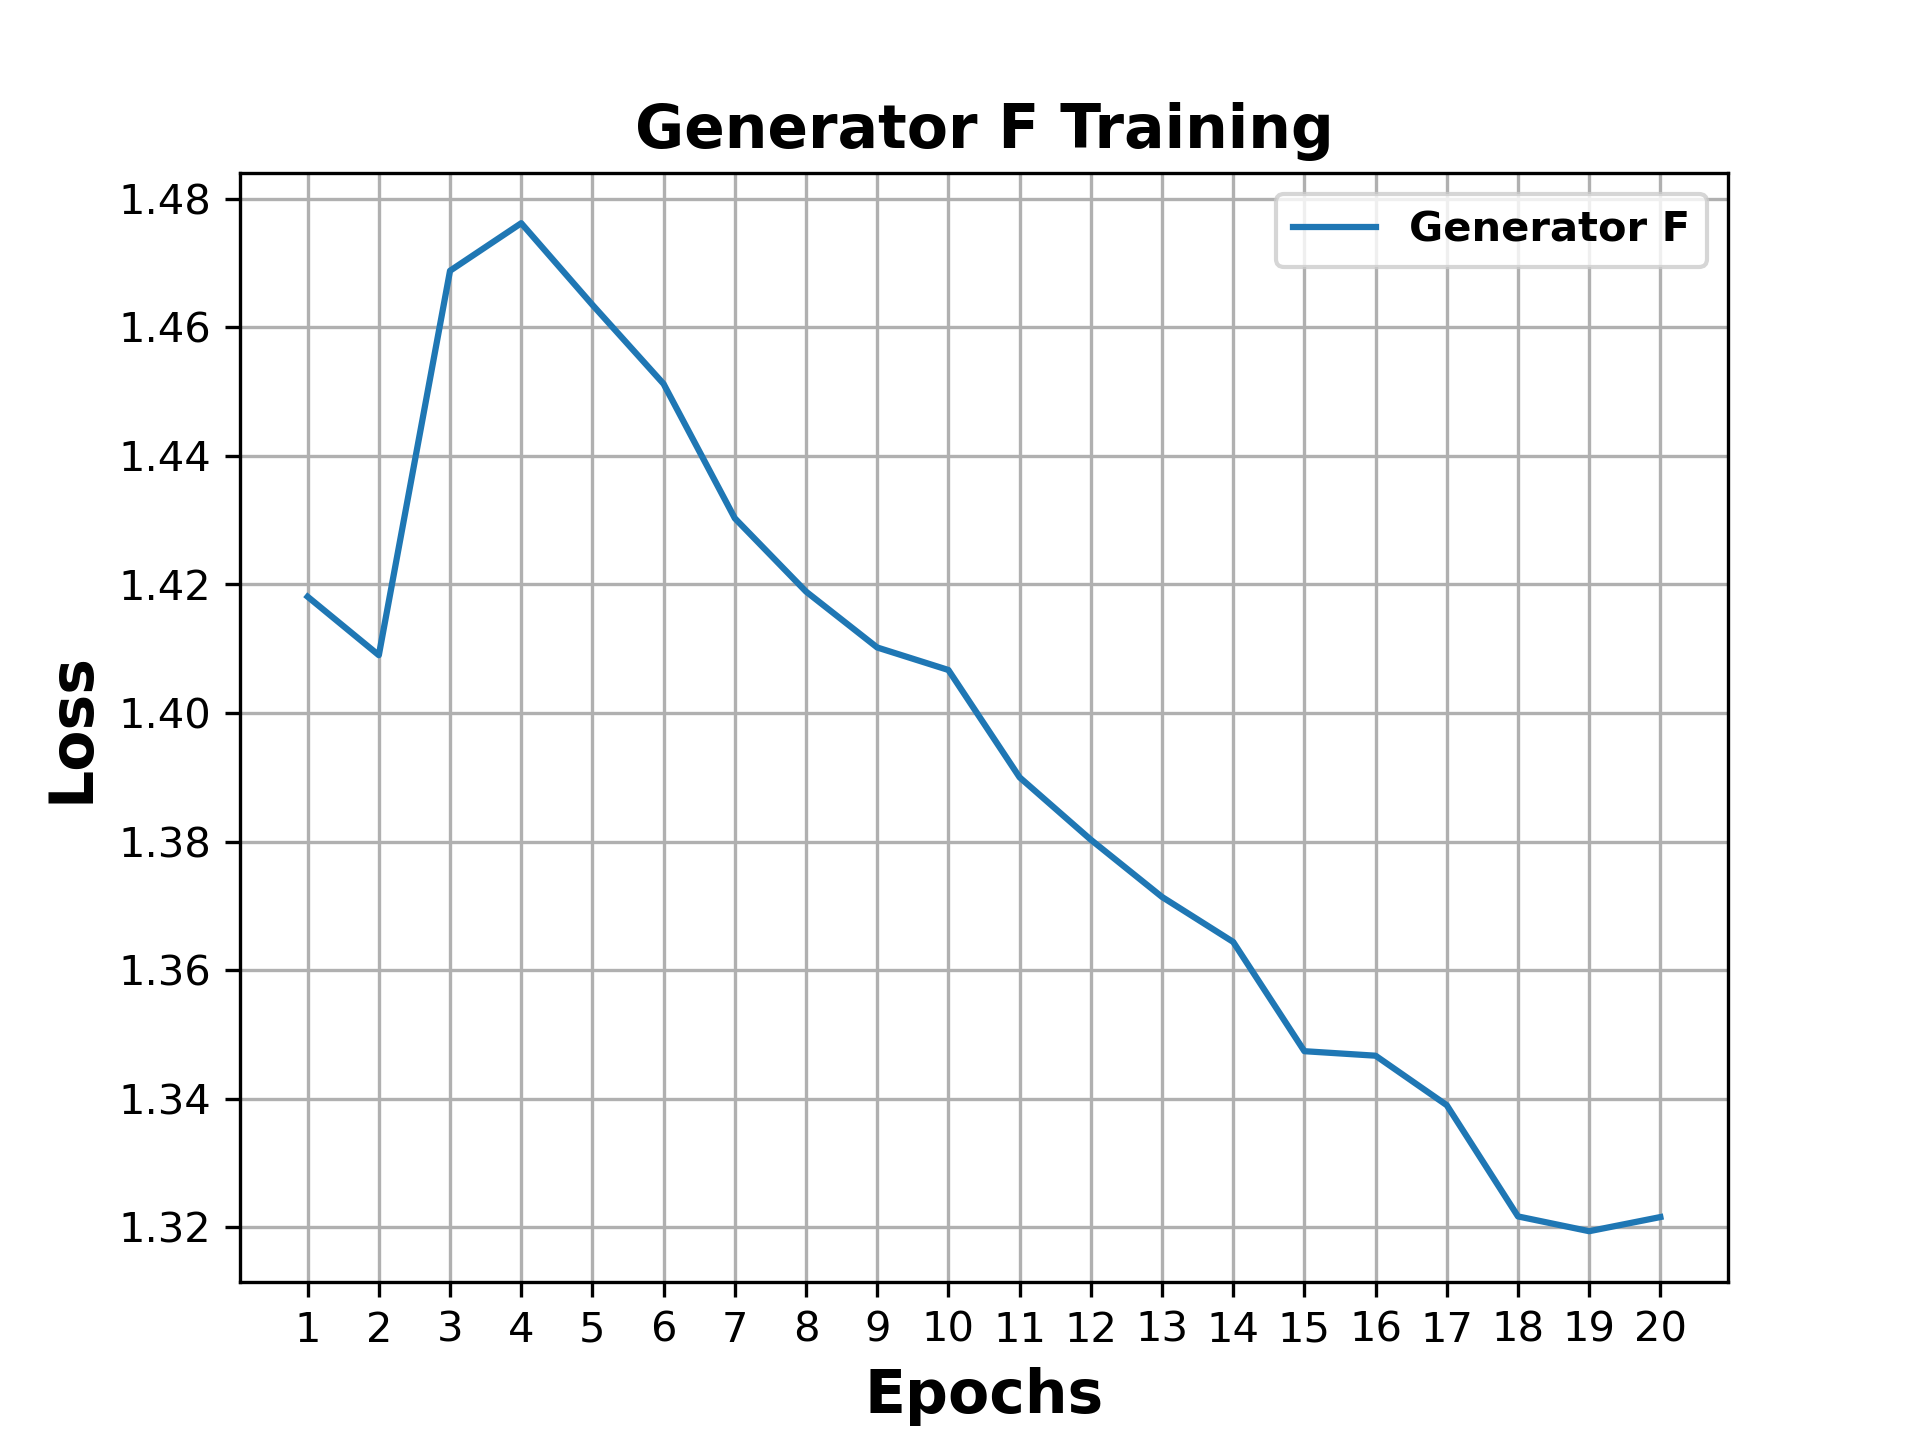
\includegraphics[width=\textwidth]{images/Evaluation/GeneratorFTraining.png}
    \caption[Epochs vs. Loss plot during Generator $F$ is training.]{Epochs vs. Loss plot during Generator $F$ is training.}
    \label{fig:generatorF}
  \end{minipage}
  \hfill
  \begin{minipage}[b]{0.49\textwidth}
    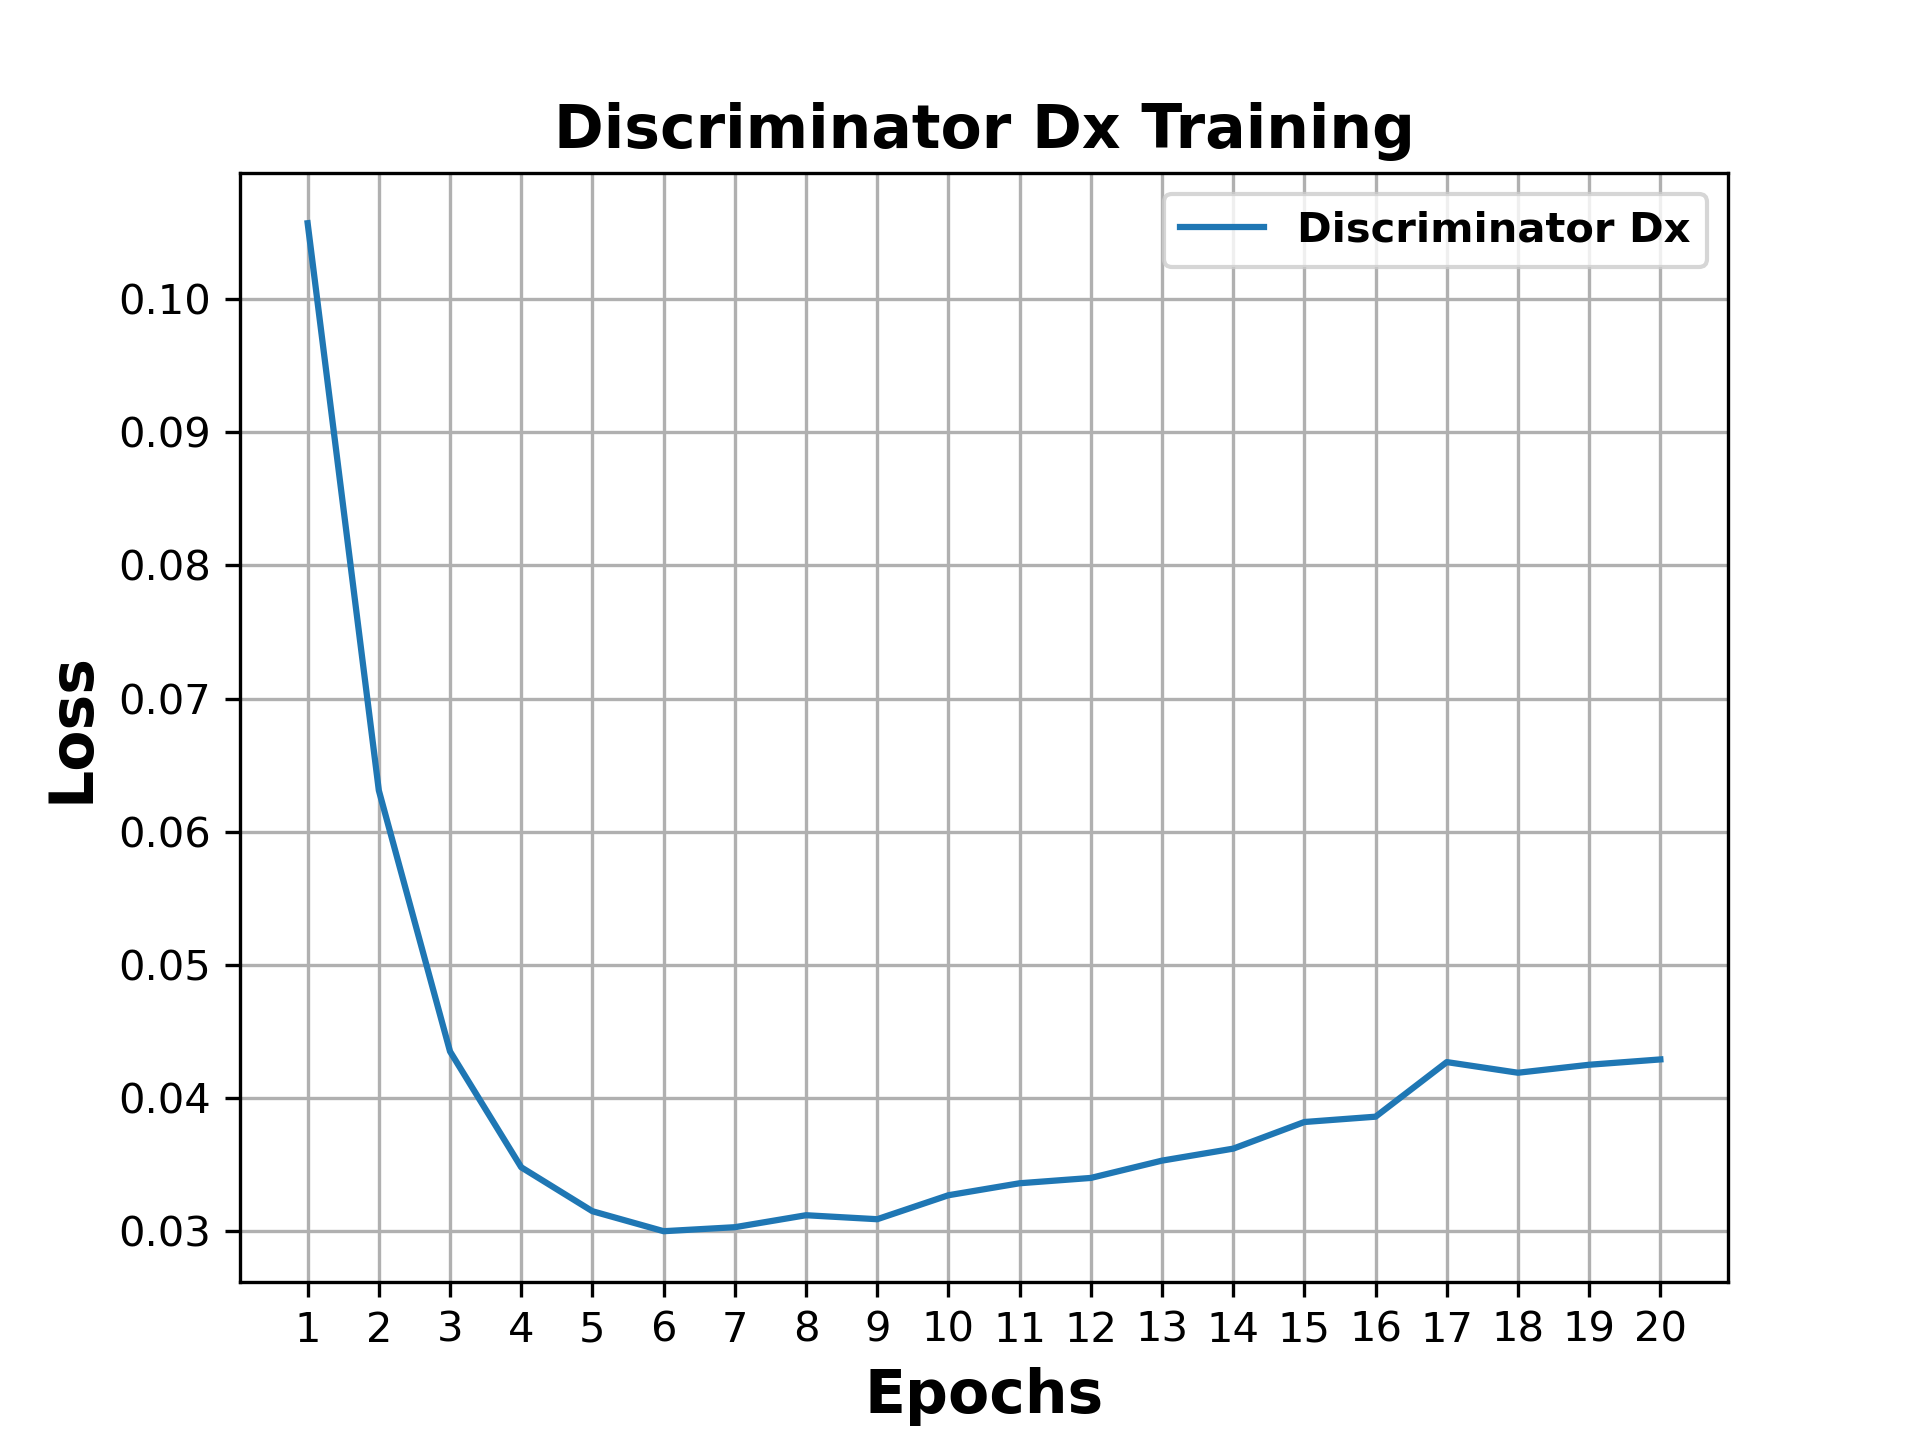
\includegraphics[width=\textwidth]{images/Evaluation/DiscriminatorDxTraining.png}
    \caption[Epochs vs. Loss plot during Discriminator $D_X$ is training.]{Epochs vs. Loss plot during Discriminator $D_X$ is training.}
    \label{fig:discriminatorDx}
  \end{minipage}
\end{figure}


Further, identity mapping loss is calculated to preserve the color of images after domain translation using generators $G$ and $F$. The generator $G$ transforms the image from domain $X$ to the domain $Y$. When the input $y_i$ is given to generator $G$ from the target domain $Y$, it should produce an identical image. The identity mapping loss for generator $G$ is the difference between the original image $y_i$ and the transformed image \textit{Same\_Y} when $y_i$ is used as an input for $G$. And, the identity mapping loss for generator $F$ is the difference between input image $x_i$ and the transformed image \textit{Same\_X} when $x_i$ is used as an input for $F$. The generator loss for generators $G$ and $F$ is calculated by the feedback given by their respective discriminators $D_Y$ and $D_X$. Combining generator loss, cycle-consistency loss and identity mapping loss, the total generator loss is calculated separately for generators $G$ and $F$ and their weights are updated to produce quality images. The epochs against loss plot while training generators $G$ and $F$ are shown in figure \ref{fig:generatorG} and \ref{fig:generatorF} respectively. Also, the epochs against loss plot while training discriminators $D_Y$ and $D_X$ are shown in figure \ref{fig:discriminatorDy} and \ref{fig:discriminatorDx} respectively. The algorithm of \ac{CycleGAN} is described in section \ref{CycleGANAlgorithm}. The complete architecture of the proposed image-to-image translation application using \ac{CycleGAN} is illustrated in figure \ref{fig:GxyFyx}. For more \ac{CycleGAN} training details refer section \ref{TrainingDetailsCycleGAN}. 




\subsection{Training a Classifier on \ac{CycleGAN} Generated Document Images}\label{trainingCycleGANDataClassifier}


Once \ac{CycleGAN} is trained, the generator $G$ is retrieved from the saved \ac{CycleGAN} model to transform synthetic document images to realistic document images. 100,000 synthetic document images are transformed into realistic document images. The classifier is trained using these transformed 100,000 realistic document images. The performance of this classifier is evaluated on the testing dataset (Annotated real document images) to understand the domain gap between real data distribution and \ac{CycleGAN} generated data distribution. The purpose of this experiment is to determine how closely the \ac{CycleGAN} generated data distribution matches the real data distribution. The quality of generated realistic document images can be determined using this experiment. The classification report in table \ref{table:CycleGANClassificationReport} states that the accuracy of this classifier on the testing dataset is 27\%, macro average F1-score is 34\% and weighted average F1-score is 25\%. 


The results conclude that the faxified data distribution matched the real data distribution better than the \ac{CycleGAN} generated data distribution. The confusion matrix is illustrated in figure \ref{fig:CMFaxifiedDocumentImagesClassifier}. In which, the document images DE\_LY\_Arm\_2020-01 (support 44 and recall 75\%), DE\_LY\_Bein\_2019-07 (support 60 and recall 83\%), DE\_LY\_Hand\_2020-01 (support 16 and recall 75\%), DE\_PH\_Bein\_2019-02 (support 28 and recall 46\%) and DE\_PH\_Bein\_2020-01 (support 143 and recall 67\%) are classified satisfactorily, with convincing recall score. Document images DE\_LY\_Bein\_2020-01 and DE\_LY\_Bein\_2020-03 are wrongly classified as DE\_LY\_Bein\_2019-07. Document images DE\_PH\_Bein\_2018-09 and DE\_PH\_Bein\_2019-02 are wrongly classified as DE\_PH\_Bein\_2019-02. As shown in the in confusion matrix \ref{fig:CMCycleganGeneratedDocumentImagesClassifier}, most of the generated document images DE\_LY\_Bein\_2019-01 are misclassified as DE\_LY\_Bein\_2019-07. The real document images DE\_LY\_Bein\_2019-01 and DE\_LY\_Bein\_2019-07 are similar to each other with couple of minor differences. Examples of DE\_LY\_Bein\_2019-01 and DE\_LY\_Bein\_2019-07 real document images are illustrated in figure \ref{fig:MissclassificationExample}. It is challenging for \ac{CycleGAN} to learn such minor differences and features from large training datasets. Also, the majority of document images are of the type ``Bein'' and they are similar to each other, learning minor differences and features between them from the training dataset is very challenging. The \ac{CycleGAN} is failed to learn such small and complex differences, hence some of the generated images are more similar to different classes than the original class and they are misclassified. In section \ref{QualitativeResults}, qualitative results of the image-to-image translation are illustrated along with failure cases. The epochs against accuracy and epochs against loss plots while training classifier on \ac{CycleGAN} generated document images is illustrated in figure \ref{fig:CycleGANClassifierAcc} and \ref{fig:CycleGANClassifierLoss} respectively.


\begin{figure}[H]
  \centering
  \begin{minipage}[b]{0.45\textwidth}
    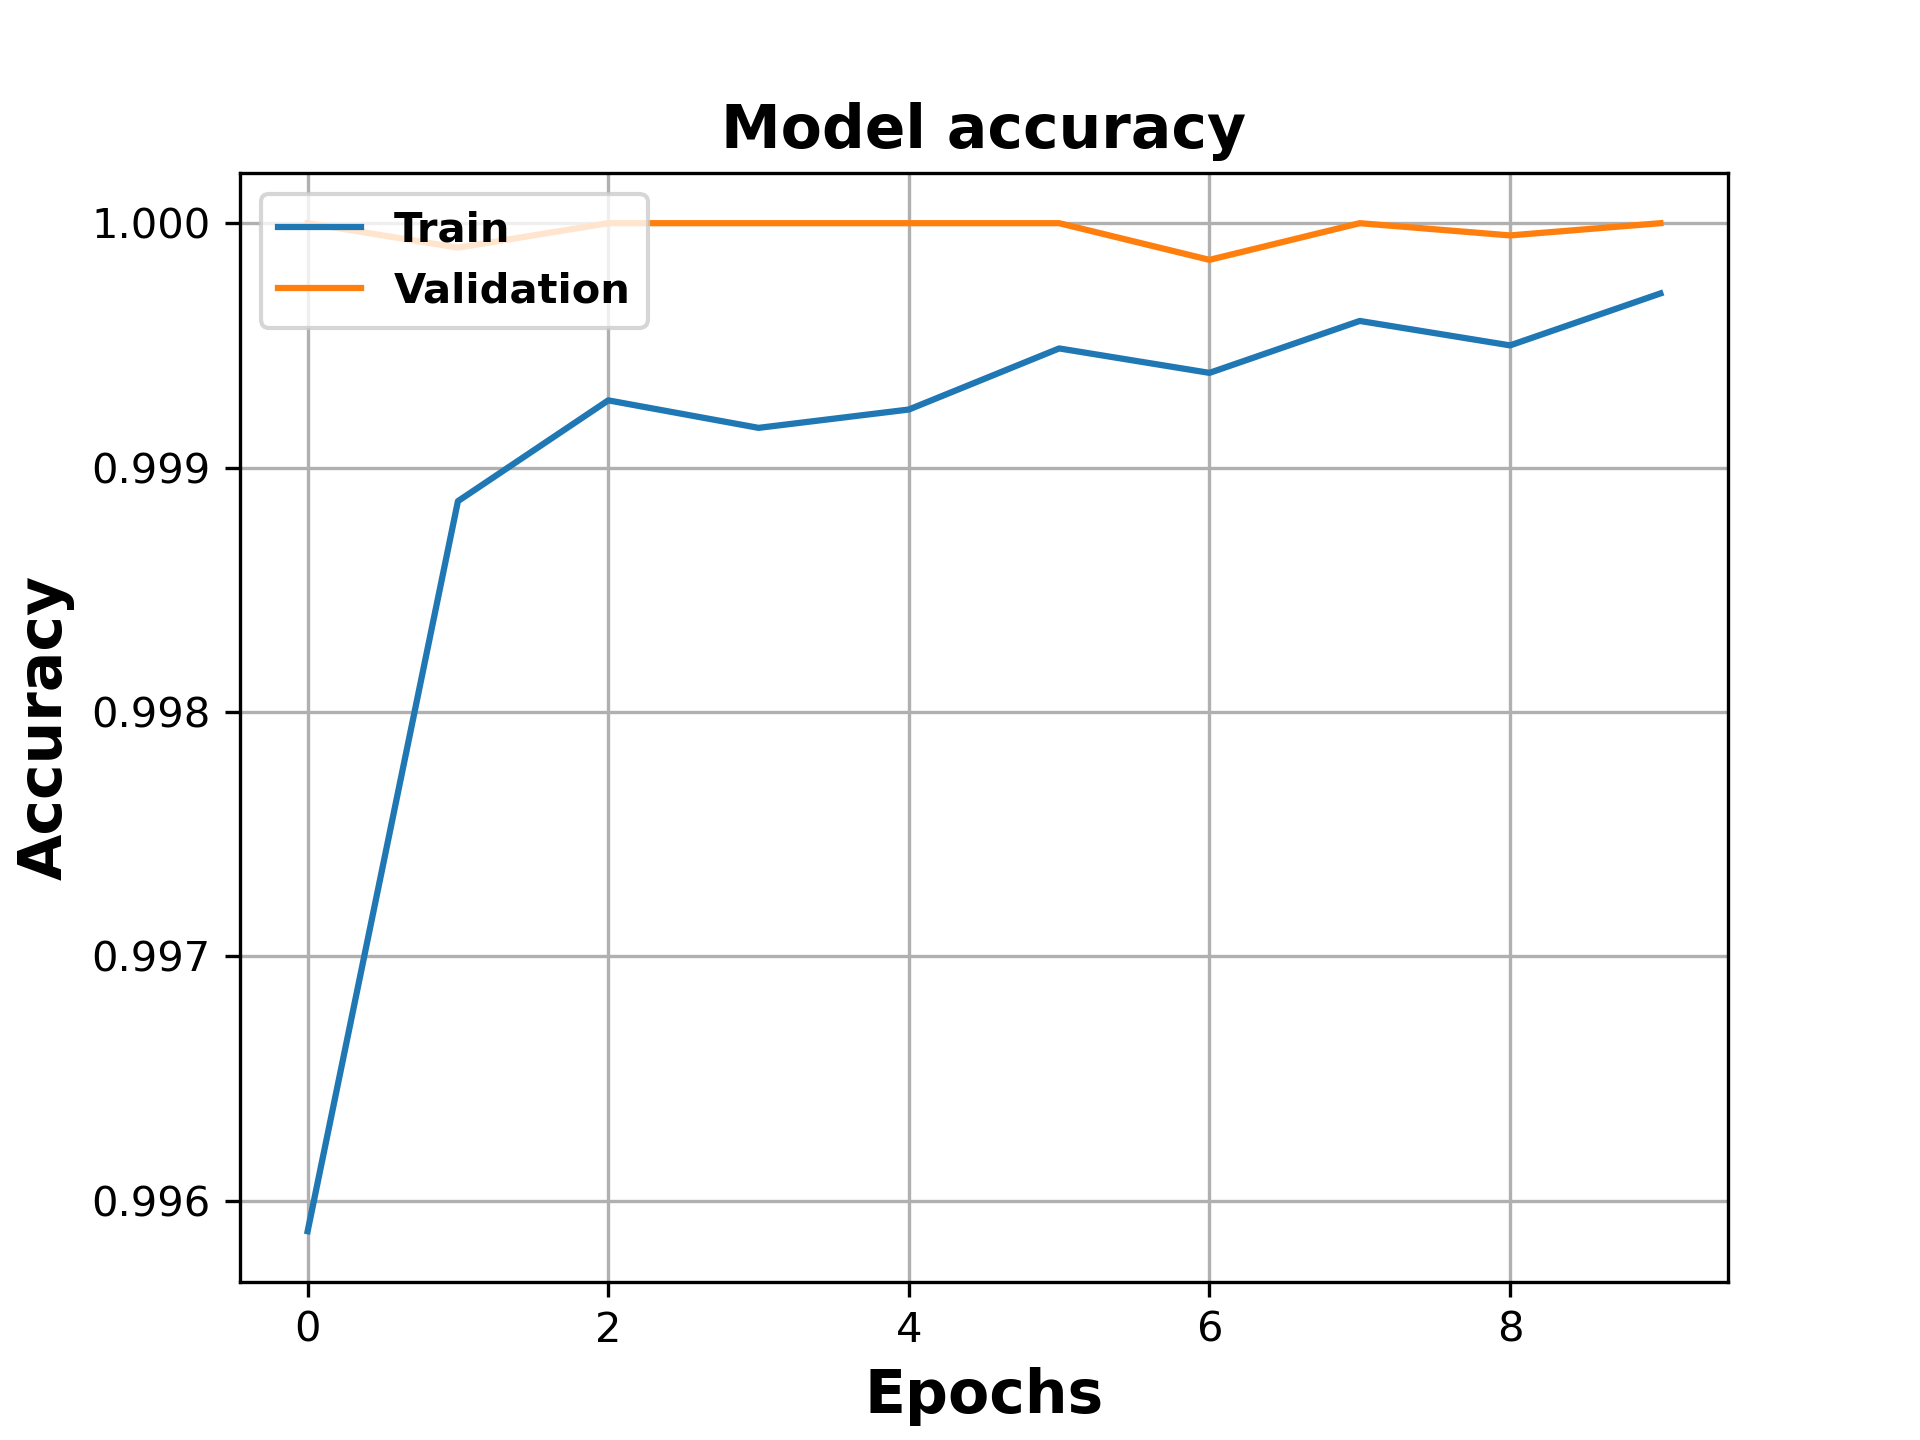
\includegraphics[width=\textwidth]{images/Evaluation/CycleGAN_Generated_Data_Classifier_2021-06-02_21-55-39_Accuracy.png}
    \caption[Epochs vs. Accuracy plot during training a classifier on \ac{CycleGAN} generated document images.]{Epochs vs. Accuracy plot during training a classifier  on \ac{CycleGAN} generated document images.}
    \label{fig:CycleGANClassifierAcc}
  \end{minipage}
  \hfill
  \begin{minipage}[b]{0.45\textwidth}
    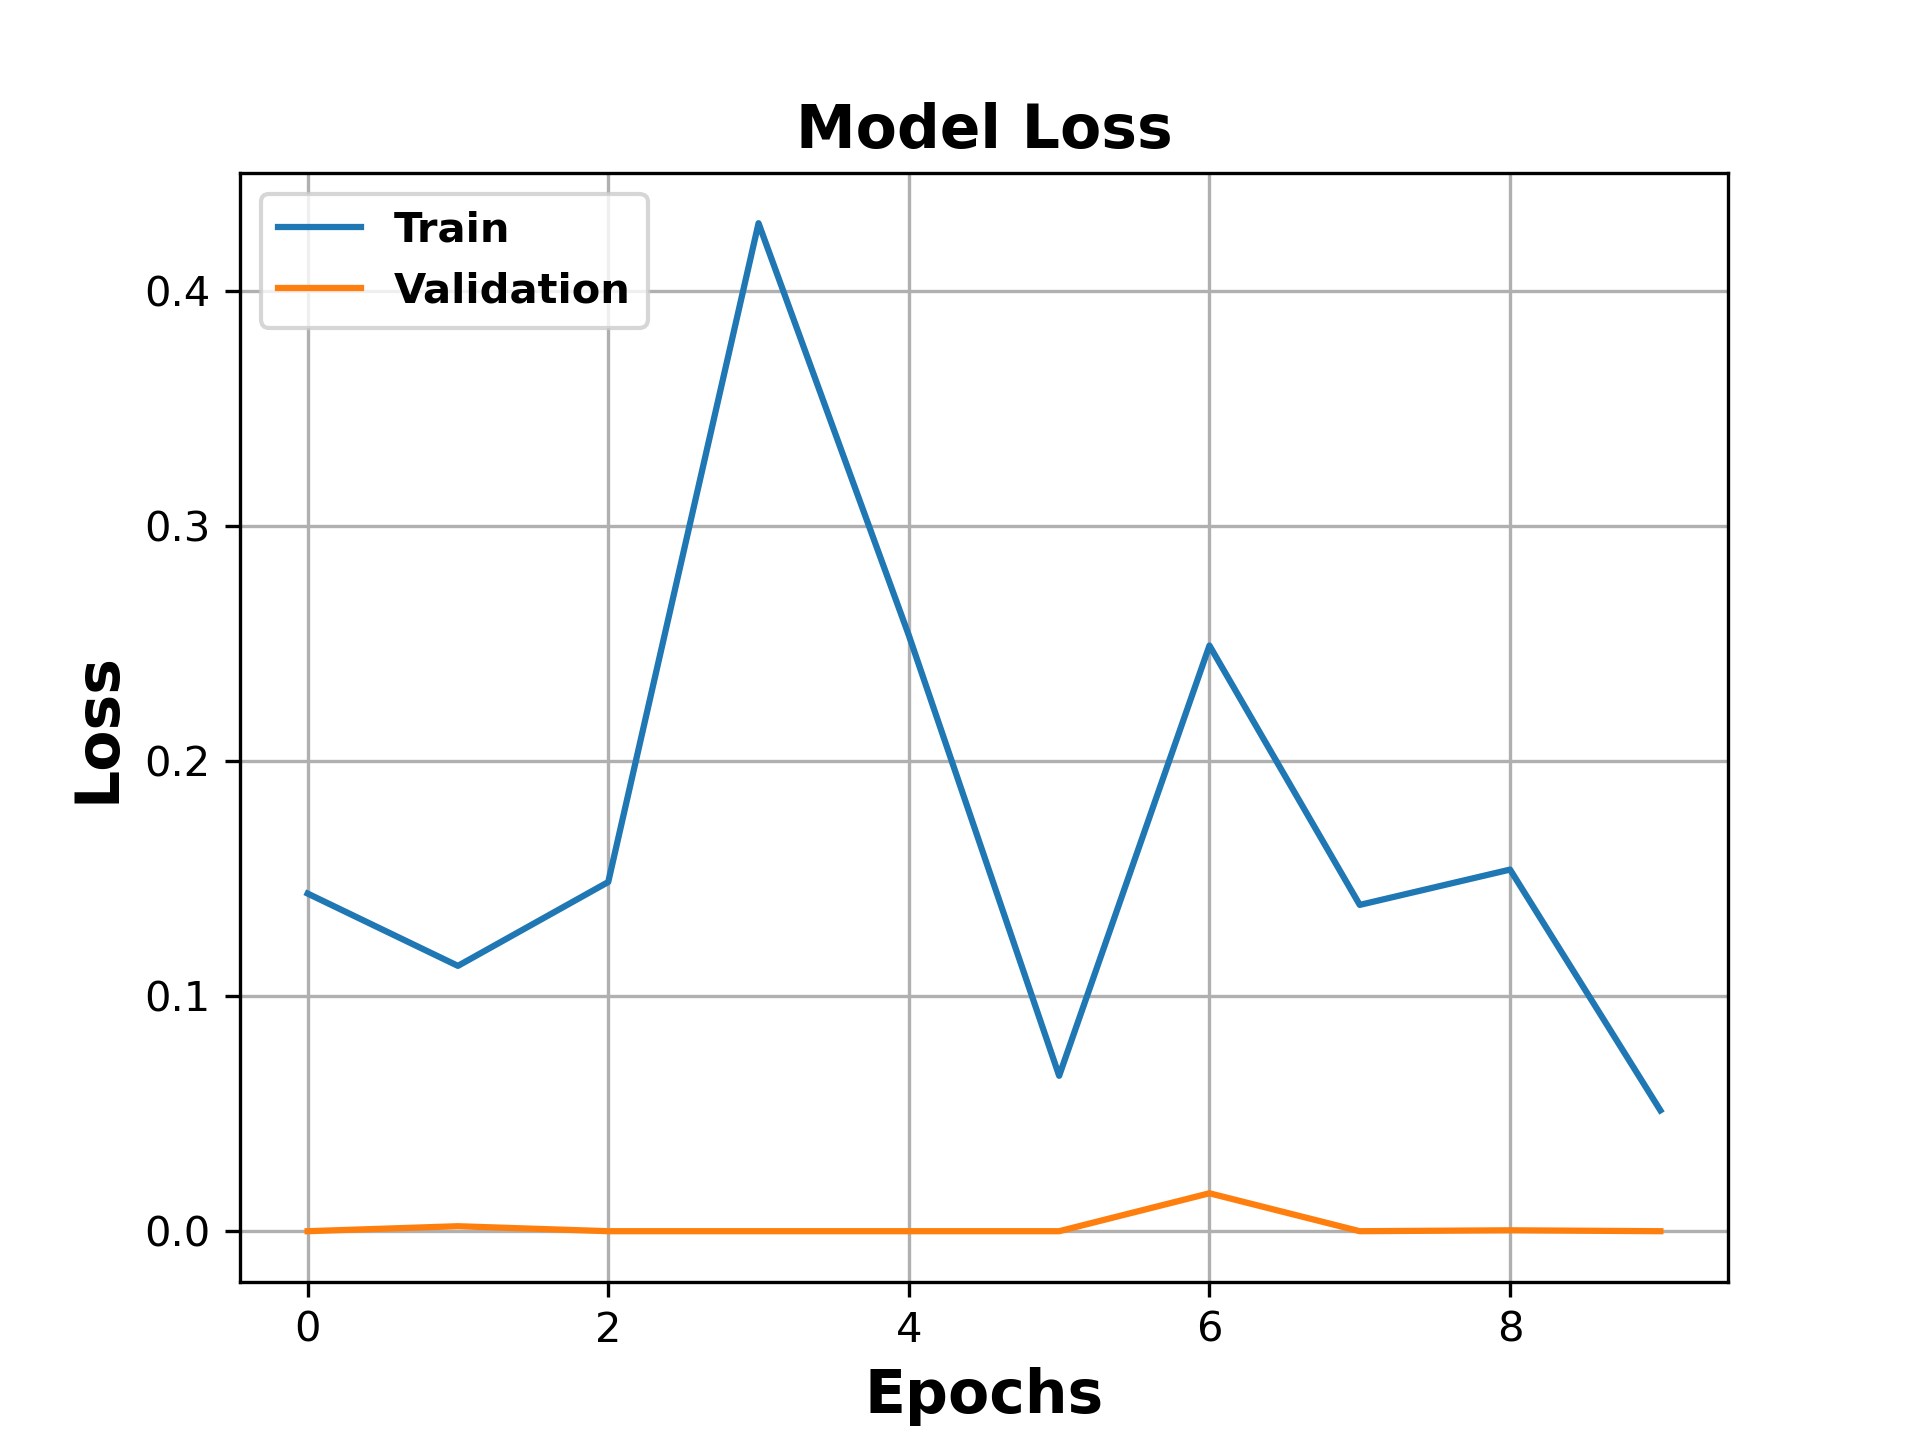
\includegraphics[width=\textwidth]{images/Evaluation/CycleGAN_Generated_Data_Classifier_2021-06-02_21-55-39_Loss.png}
    \caption[Epochs vs. Loss plot during training a classifier on \ac{CycleGAN} generated document images.]{Epochs vs. Loss plot during training a classifier on \ac{CycleGAN} generated document images.}
    \label{fig:CycleGANClassifierLoss}
  \end{minipage}
\end{figure}


\begin{figure}[H]
    \begin{center}
	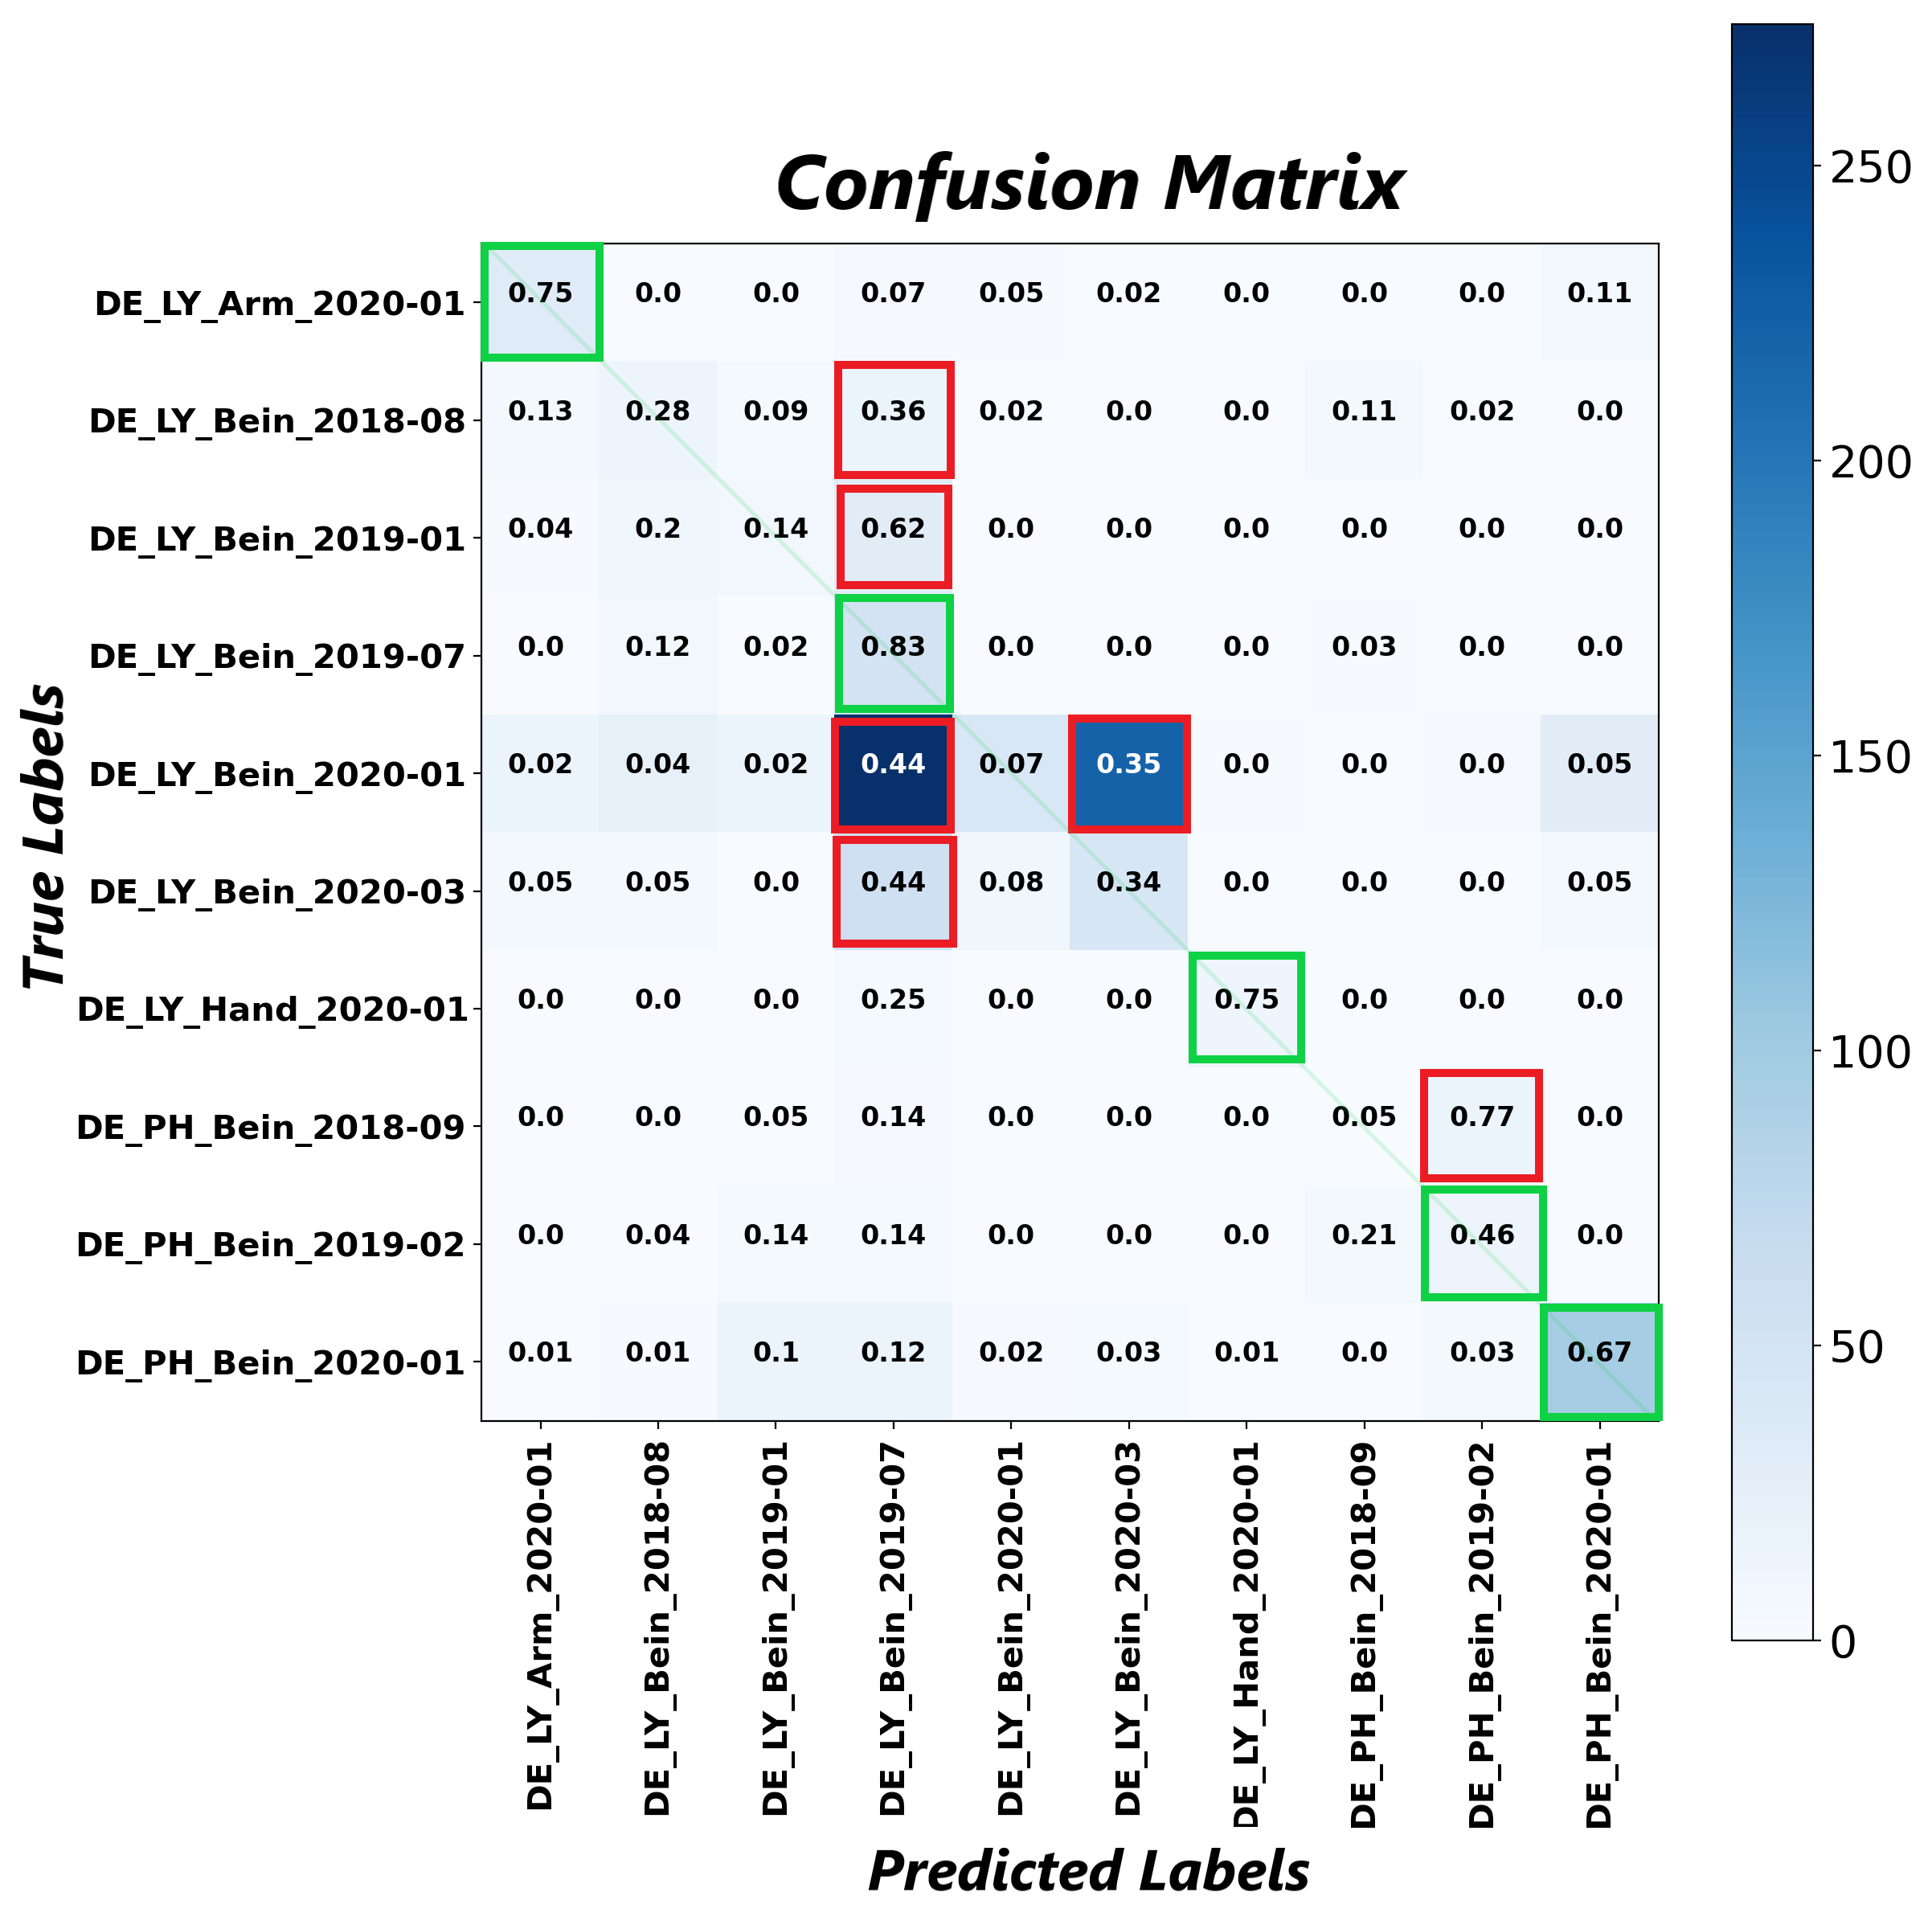
\includegraphics[scale=0.70]{images/Evaluation/Confusion_Matrix_CycleGAN_Generated_Data_Classifier_2021-06-02_21-55-39.png}
	\caption[Confusion matrix to analyze the performance of the classifier trained on \ac{CycleGAN} generated document images and evaluated using real annotated document images (test dataset).]{Confusion matrix to analyze the performance of the classifier trained on \ac{CycleGAN} generated document images and evaluated using real annotated document images (testing dataset).}
	\label{fig:CMCycleganGeneratedDocumentImagesClassifier}
	\end{center}
\end{figure}

\begin{center}
\begin{table}[H]
    \begin{center}
    \begin{tabular}{P{0.22\linewidth} P{0.10\linewidth} P{0.10\linewidth} P{0.10\linewidth} P{0.10\linewidth}} 
	        \toprule
            & Precision & Recall & F1-score & Support\\[0.0ex] 
        \midrule
        DE\_LY\_Arm\_2020-01 & 0.53 & 0.75 & 0.62 & 44\\[0.0ex]
        \midrule
        DE\_LY\_Bein\_2018-08 & 0.21 & 0.28 & 0.24 & 47\\[0.0ex]
        \midrule
        DE\_LY\_Bein\_2019-01 & 0.16 & 0.14 & 0.15 & 50\\[0.0ex]
        \midrule
        DE\_LY\_Bein\_2019-07 & 0.11 & 0.83 & 0.19 & 60\\[0.0ex]
        \midrule
        DE\_LY\_Bein\_2020-01 & 0.72 & 0.07 & 0.12 & 624\\[0.0ex]
        \midrule
        DE\_LY\_Bein\_2020-03 & 0.16 & 0.34 & 0.22 & 128\\[0.0ex]
        \midrule
        DE\_LY\_Hand\_2020-01 & 0.80 & 0.75 & 0.77 & 16\\[0.0ex]
        \midrule
        DE\_PH\_Bein\_2018-09 & 0.07 & 0.05 & 0.06 & 22\\[0.0ex]
        \midrule
        DE\_PH\_Bein\_2019-02 & 0.33 & 0.46 & 0.39 & 28\\[0.0ex]
        \midrule
        DE\_PH\_Bein\_2020-01 & 0.70 & 0.67 & 0.68 & 143\\[0.0ex]
        \midrule
        \midrule
        Accuracy              &      &      & \bf{0.27} & 1162\\[0.0ex]
        Macro average             & 0.38 & 0.43 &  \bf{0.34} & 1162\\[0.0ex]
        Weighted average          & 0.55 & 0.27 &  \bf{0.25} & 1162\\[0.0ex]
        \bottomrule
    \end{tabular}
    \caption[Classification report, evaluating a classifier on the testing dataset after training with \ac{CycleGAN} generated document images.]{Classification report, evaluating a classifier on the testing dataset after training with \ac{CycleGAN} generated document images.}
    \label{table:CycleGANClassificationReport}
    \end{center}
\end{table}
\end{center}

\vspace*{2cm}

\begin{figure}[H]
    \begin{center}
	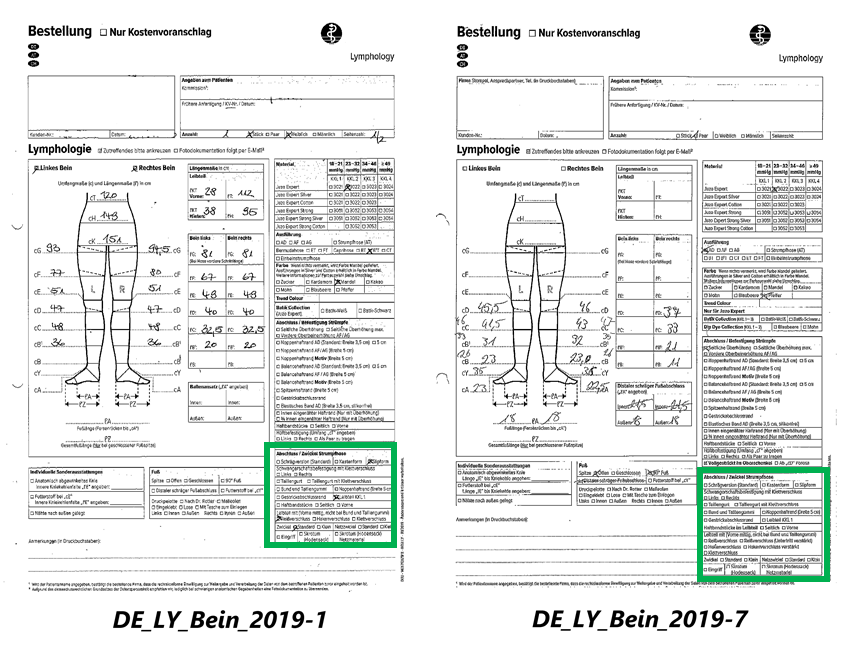
\includegraphics[scale=0.50]{images/Evaluation/MissclassificationExample.png}
	\caption[Examples of DE\_LY\_Bein\_2019-01 and DE\_LY\_Bein\_2019-07 real document images.]{Examples of DE\_LY\_Bein\_2019-01 and DE\_LY\_Bein\_2019-07 real document images. Both real document images are similar to each other hence learning such minor differences from the training dataset is a challenging for \ac{CycleGAN}.}
	\label{fig:MissclassificationExample}
	\end{center}
\end{figure}


\newpage
\section{Results}\label{results}

This section discusses the qualitative and quantitative results of the proposed image-to-image translation application implemented using \ac{CycleGAN}. In experiments, three separate classifiers are trained on three data distributions, synthetic data distribution, faxified data distribution and \ac{CycleGAN} generated data distribution. The performance of these classifiers that are trained using different distributions is evaluated and compared using the testing dataset (Annotated real document images) to analyze the domain gap between these distributions and real data distribution. The experiment of training a classifier on \ac{CycleGAN} generated document images and evaluating on testing dataset helps to determine the quality of \ac{CycleGAN} generated document images. It shows how close the generated document images are to the real document images.

The performance of the classifiers is evaluated using metrics like accuracy, macro average F1-score and weighted average F1-score. The accuracy of a classifier trained on synthetic document images is 25\%, the accuracy of a classifier trained on faxified document images is 27\% and the accuracy of a classifier trained on \ac{CycleGAN} generated document images is 43\%. The accuracy is not a good metric to evaluate the performance of the classifiers when imbalanced datasets are involved\footnote{\url{https://machinelearningmastery.com/failure-of-accuracy-for-imbalanced-class-distributions/} \dcdate}. The performance evaluation of the classifiers trained on different data distributions is calculated using an imbalanced testing dataset. Hence, it will be beneficial to consider macro average and weighted average F1-score metrics to evaluate the performance of the classifiers. The macro average F1-score of a classifier trained on synthetic document images is 27\%, the macro average F1-score of a classifier trained on faxified document images is 34\% and the macro average F1-score of a classifier trained on \ac{CycleGAN} generated document images is 58\%. The weighted average F1-score states, 25\% real document images were correctly classified when a classifier is trained using \ac{CycleGAN} generated document images. 43\% real document images were correctly classified when a classifier is trained using faxified document images. 31\% real document images were correctly classified when a classifier is trained using synthetic document images. Finally, results conclude that the quantitatively \ac{CycleGAN} generated data distribution could not match real data distribution thoroughly. The faxified data distribution produced by faxifying synthetic document images convincingly matched the real data distribution, therefore, the faxified document images are more similar to the real document images compared to \ac{CycleGAN} generated document images. The quantitative results are illustrated using a table and bar plot in section \ref{QuantitativeResults}. The proposed image-to-image translation application can be improved further in the future using different methods and loss functions. The future work and conclusion are discussed in the chapter \ref{conclusion}.


\subsection{Quantitative Evaluation}\label{QuantitativeResults}


\begin{table}[H]
\begin{tabular}{P{0.25\linewidth} P{0.20\linewidth} P{0.20\linewidth} P{0.20\linewidth}} 
	\toprule
	\bf{Data distributions} & \bf{Accuracy}  & \bf{Macro average F1-score} & \bf{Weighted average F1-score}\\[0.0ex] 
	\midrule
     \bf{Synthetic document images} & 25\% & 27\% & 31\%\\[0.0ex]
     \midrule
     \bf{\ac{CycleGAN} generated document images} & 27\% & 34\% & 25\%\\[0.0ex]
     \midrule
     \bf{Faxified document images} & 43\% & 58\% & 43\%\\[0.0ex]
     \bottomrule
\end{tabular}
 \caption[The accuracies and F1-scores when the classifiers trained on different data distributions and evaluated on testing dataset (Annotated real document images).]{The accuracies and F1-scores when the classifiers trained on different data distributions and evaluated on testing dataset (Annotated real document images).}
    \label{table:finalResults}
\end{table}



The qualitative results are illustrated in section \ref{QualitativeResults}, to understand the visual quality of document images generated using \ac{CycleGAN}. Some sample synthetic document images are transformed into realistic document images by using the proposed image-to-image translation application. Qualitatively the images generated are very distinct and mode collapse \cite{thanhtung2020catastrophic} is not observed. The generated realistic images are in the context, because of cycle-consistency loss. Major image artifacts from the synthetic document images are transformed successfully in the target domain and one can visibly determine the class of generated images. The bold strings, the logo and the QR code present in the synthetic document images are transformed and reconstructed properly in the generated images. The quality of generated document images is adequate for initial research. There is an area for improvement and further research. There are some typical failure cases of the proposed method. For example, figure \ref{fig:failure1} illustrates that, the proposed image-to-image translation application using \ac{CycleGAN} has failed to transform handwritten crops present in the synthetic document images in the target domain. The handwritten crops are very minor artifacts. It is a challenging task to learn such features. The typical failure cases of the proposed image-to-image transformation are illustrated in section \ref{FailureCases}. For example, in figure \ref{fig:failure2} the transformed image has undesired noisy artifacts, in figure \ref{fig:failure3} transformed image has a dark border and noisy artifacts and figure \ref{fig:failure4} illustrates transformed image has random artifacts that are not present in the synthetic document image. 


\vspace*{1.5cm}
\begin{figure}[H]
        \begin{center}
	    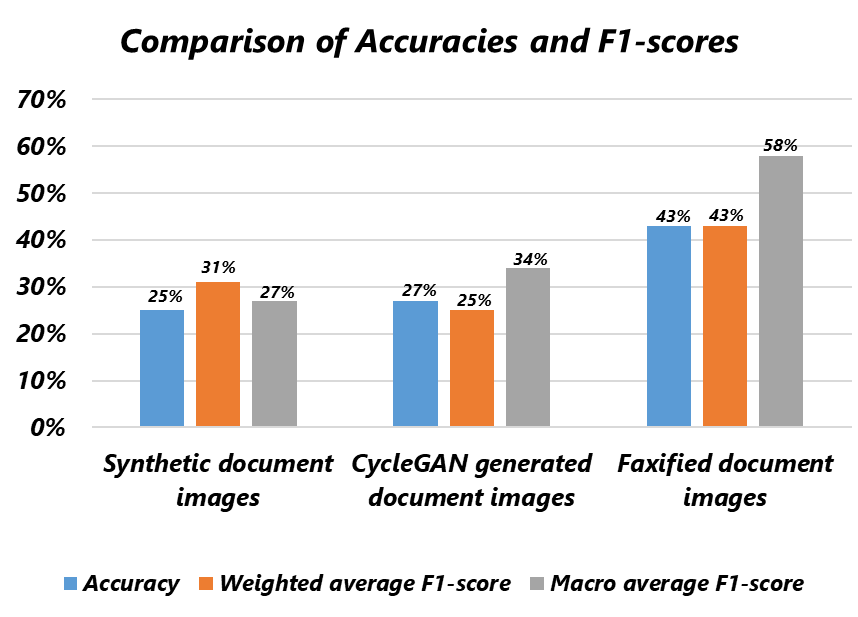
\includegraphics[scale=0.60]{images/Evaluation/ComparisonOfAccuracyAndF1Score.png}
	    \caption[Comparison of accuracies and F1-scores, when the classifiers trained on different data distributions and evaluated on testing dataset (Annotated real document images).]{Comparison of accuracies and F1-scores, when the classifiers trained on different data distributions and evaluated on testing dataset (Annotated real document images).}
	    \label{fig:ComparisonOfAccuracyAndF1Score}
	    \end{center}
\end{figure}


%The evaluation metrics like accuracy, macro average F1-score and weighted average F1-score are used.
%As the testing dataset of annotated real document images is unbalanced we consider weighted average F1-score for comparison.


\subsection{Qualitative Evaluation}\label{QualitativeResults}




\begin{figure}[H]
        \begin{center}
	    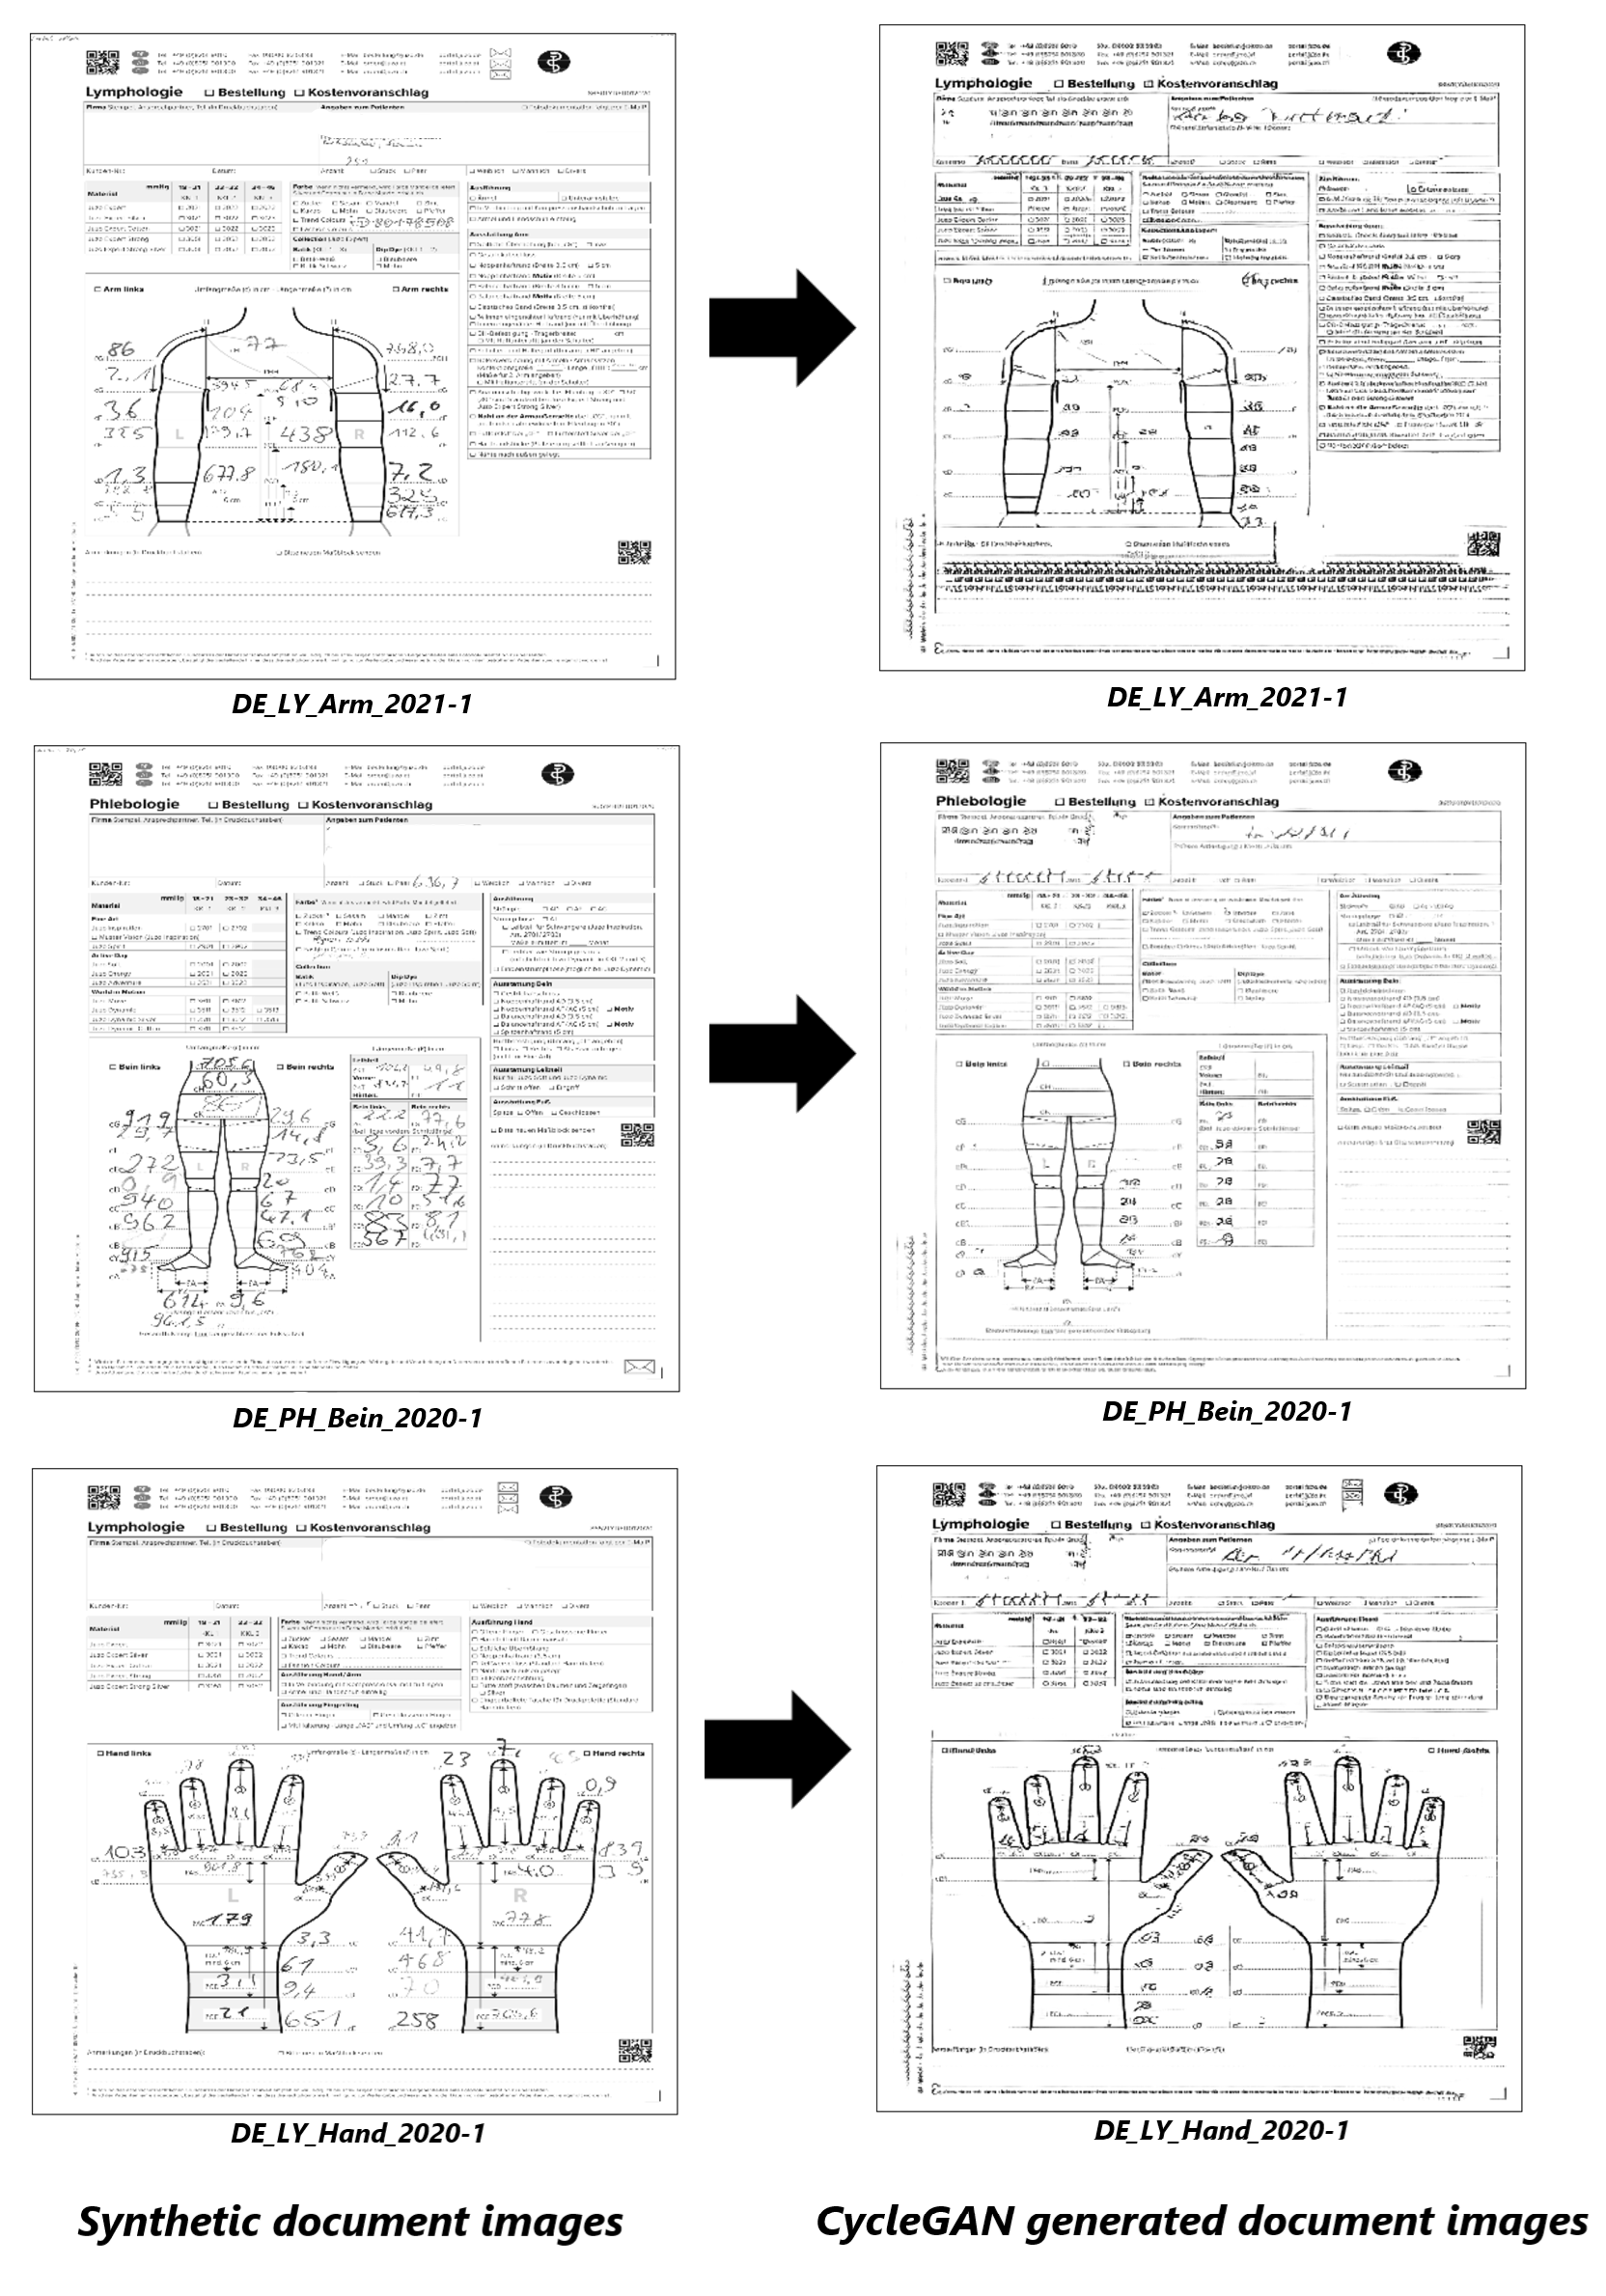
\includegraphics[scale=0.33]{images/Evaluation/Qualitative_Results.png}
	    \caption[Synthetic document images are transformed into realistic document images by the proposed image-to-image translation application.]{Synthetic document images transformed into realistic document images by the image-to-image translation application (figure reproduced from elevait GmbH \& Co. KG with permission).}
	    \label{fig:QualitativeResults}
	    \end{center}
\end{figure}

\begin{figure}[H]
        \begin{center}
	    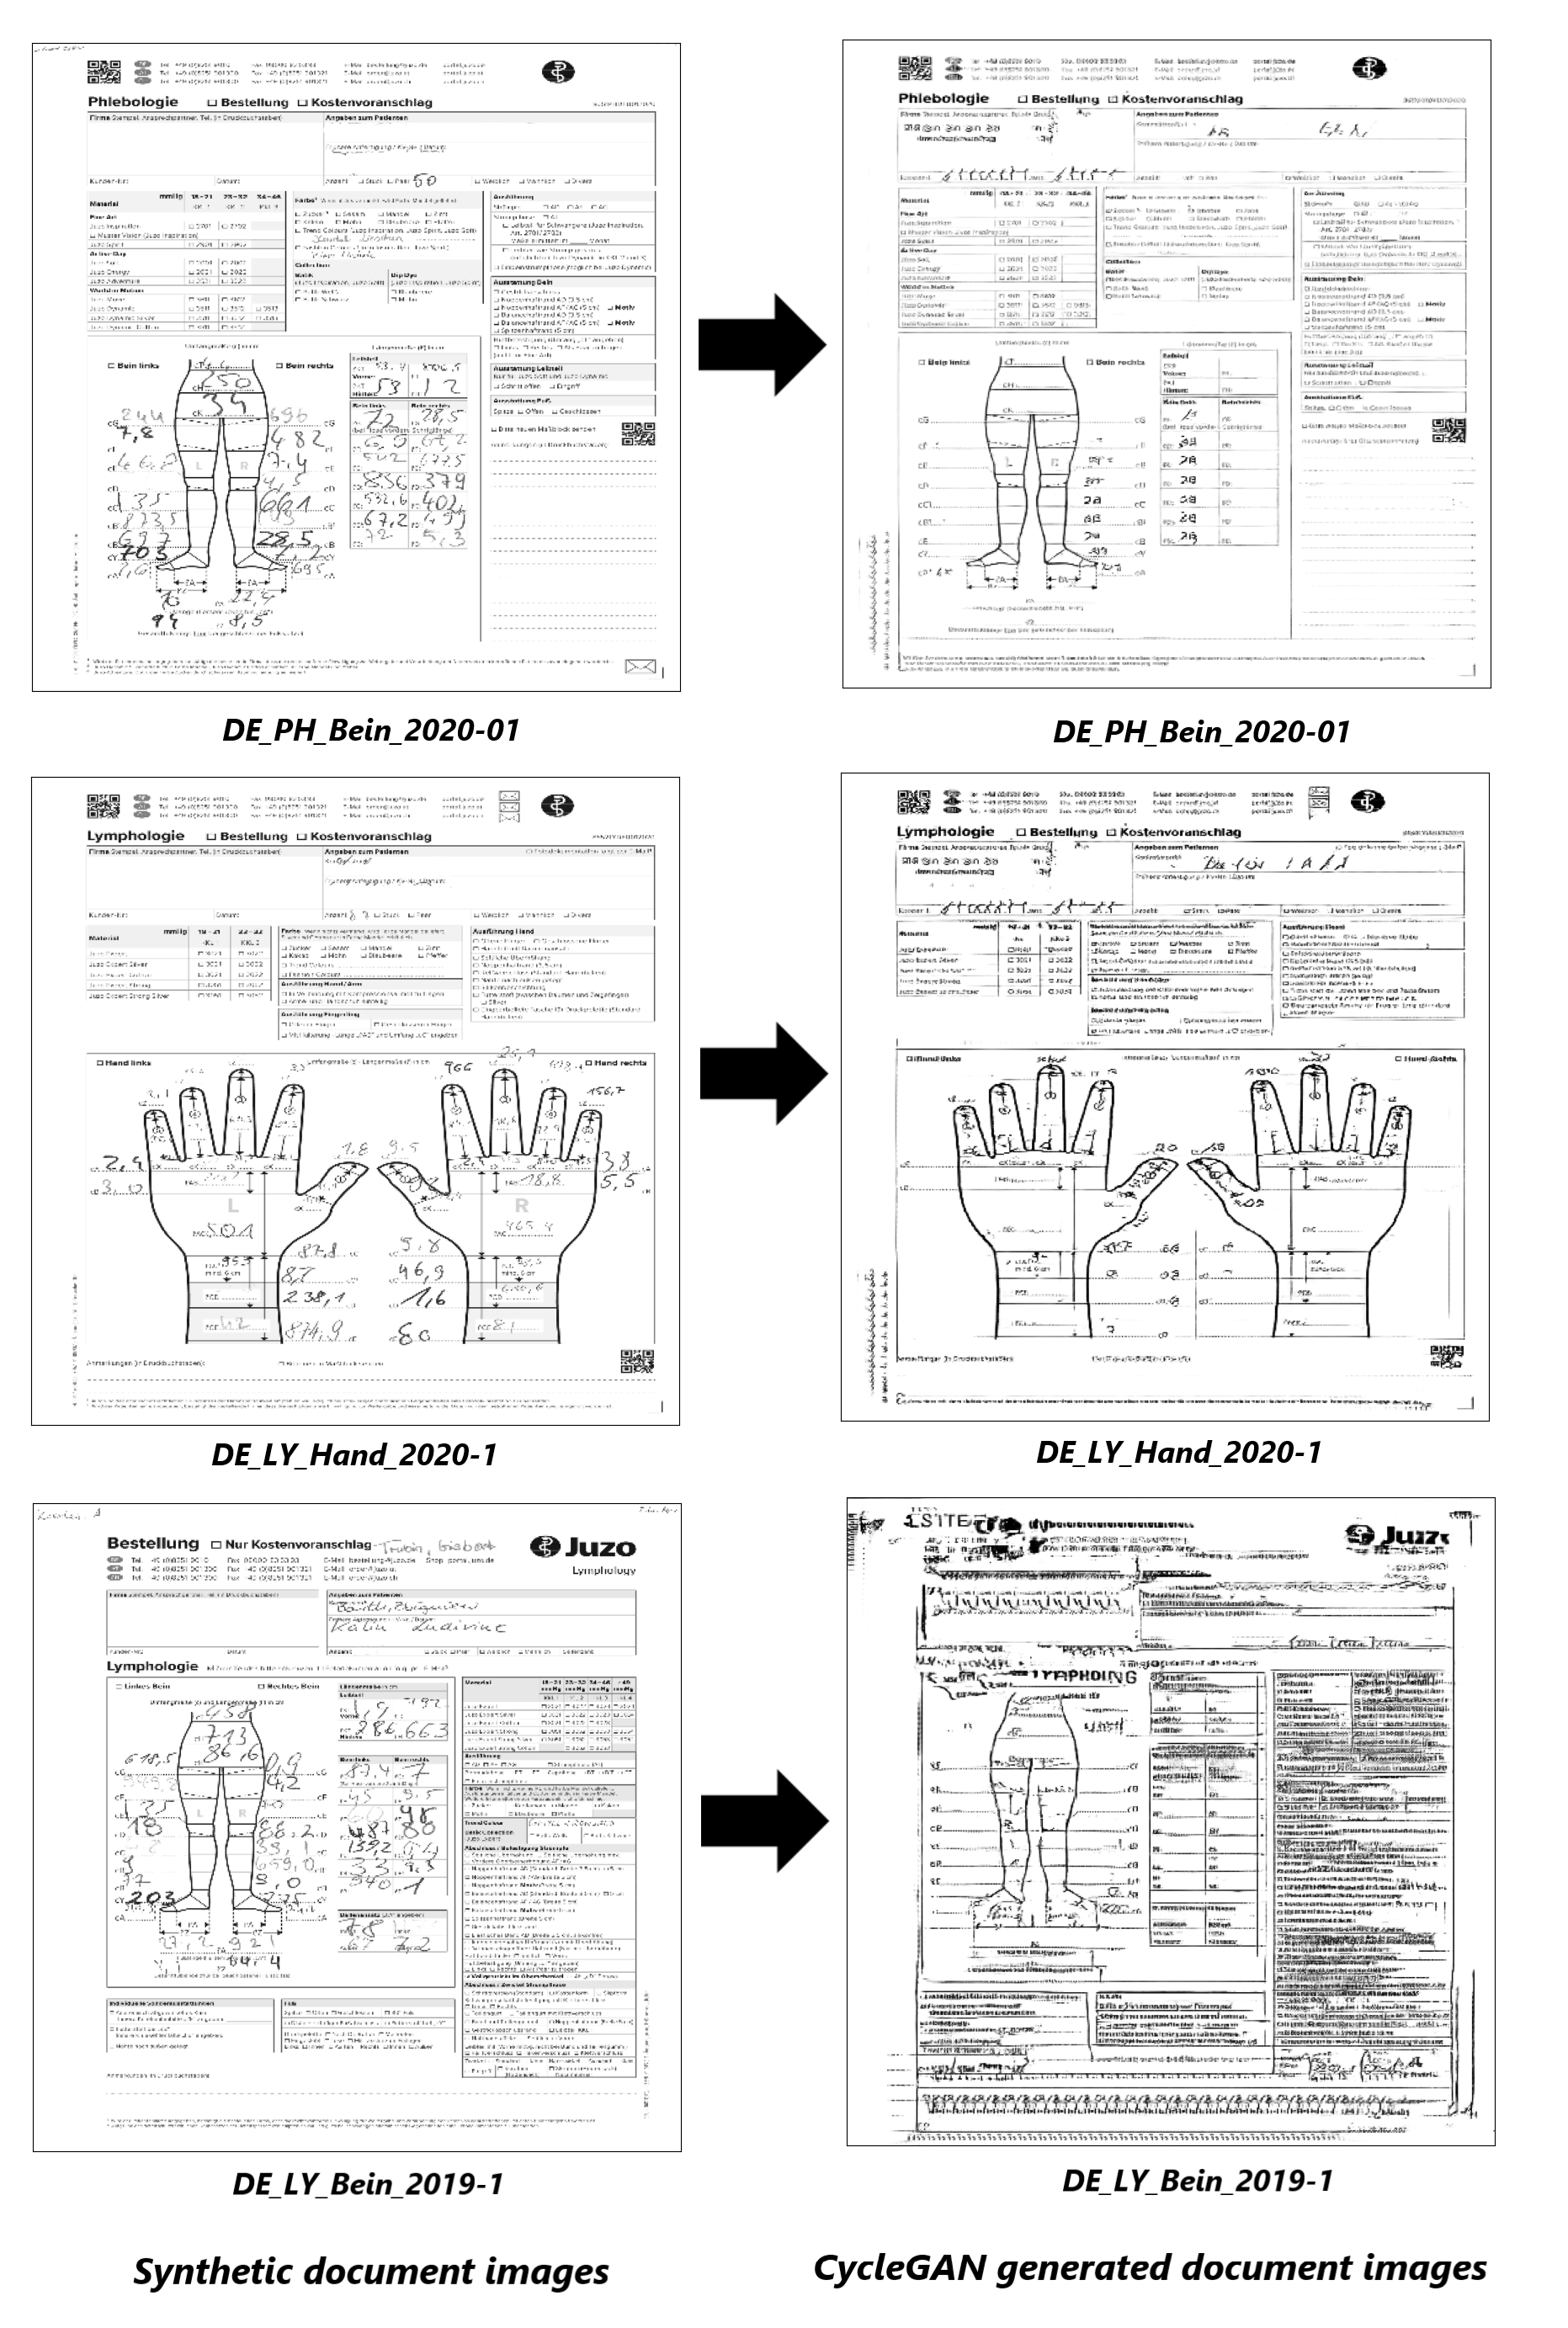
\includegraphics[scale=0.30]{images/Evaluation/Qualitative_Results_1.png}
	    \caption[Synthetic document images transformed into realistic document images by the image-to-image translation application.]{Synthetic document images transformed into realistic document images by the image-to-image translation application (figure reproduced from elevait GmbH \& Co. KG with permission).}
	    \label{fig:QualitativeResults1}
	    \end{center}
\end{figure}








\subsection{Failure Cases}\label{FailureCases}

\begin{figure}[H]
        \begin{center}
	    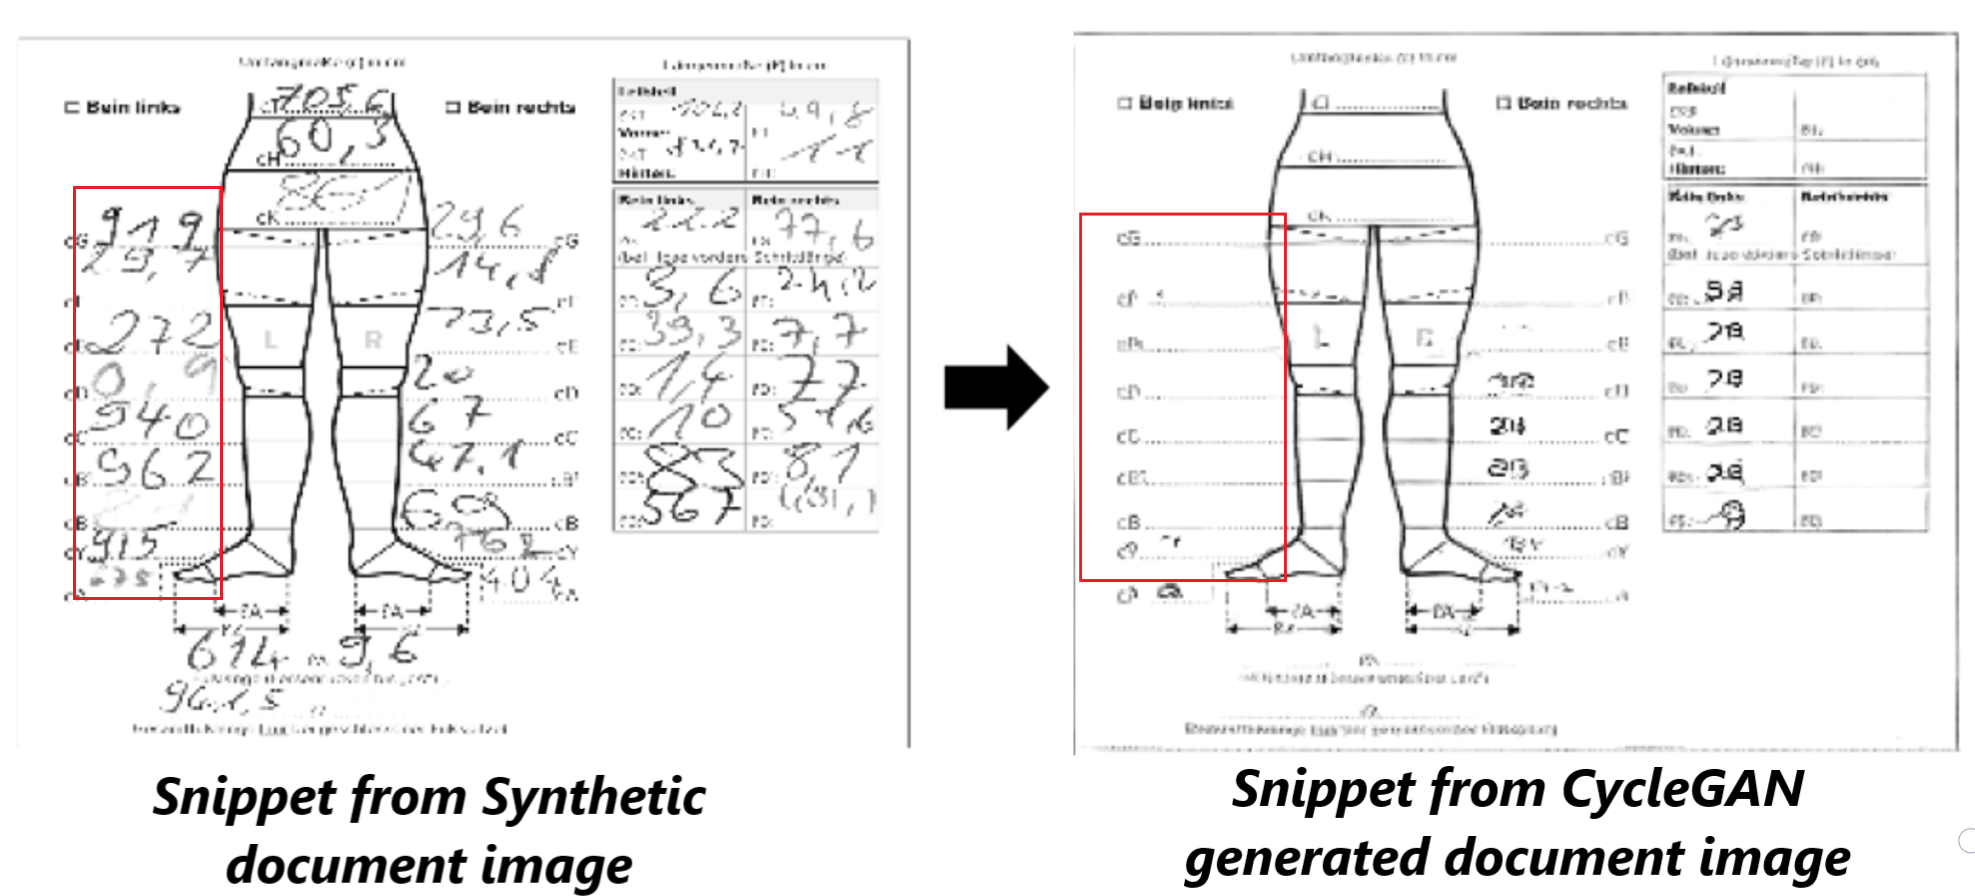
\includegraphics[scale=0.28]{images/Evaluation/failure1.png}
	    \caption[The snippet from \ac{CycleGAN} generated document image illustrates that the proposed image-to-image translation application did not transform or reconstruct handwritten crops in the target domain from the synthetic document image in the source domain.]{The snippet from \ac{CycleGAN} generated document image illustrates that the proposed image-to-image translation application did not transform or reconstruct handwritten crops in the target domain from the synthetic document image in the source domain (figure reproduced from elevait GmbH \& Co. KG with permission).}
	    \label{fig:failure1}
	    \end{center}
\end{figure}

\begin{figure}[H]
        \begin{center}
	    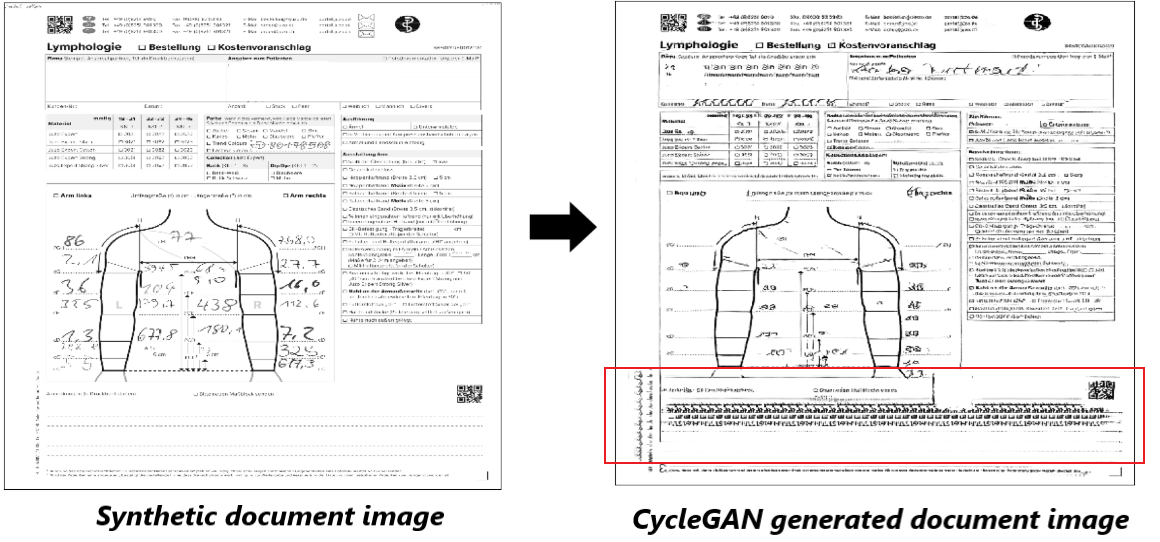
\includegraphics[scale=0.50]{images/Evaluation/failure2.png}
	    \caption[The \ac{CycleGAN} generated document image consists of noisy artifacts that are unrealistic.]{The \ac{CycleGAN} generated document image consists of noisy artifacts that are unrealistic (figure reproduced from elevait GmbH \& Co. KG with permission).}
	    \label{fig:failure2}
	    \end{center}
\end{figure}

\begin{figure}[H]
        \begin{center}
	    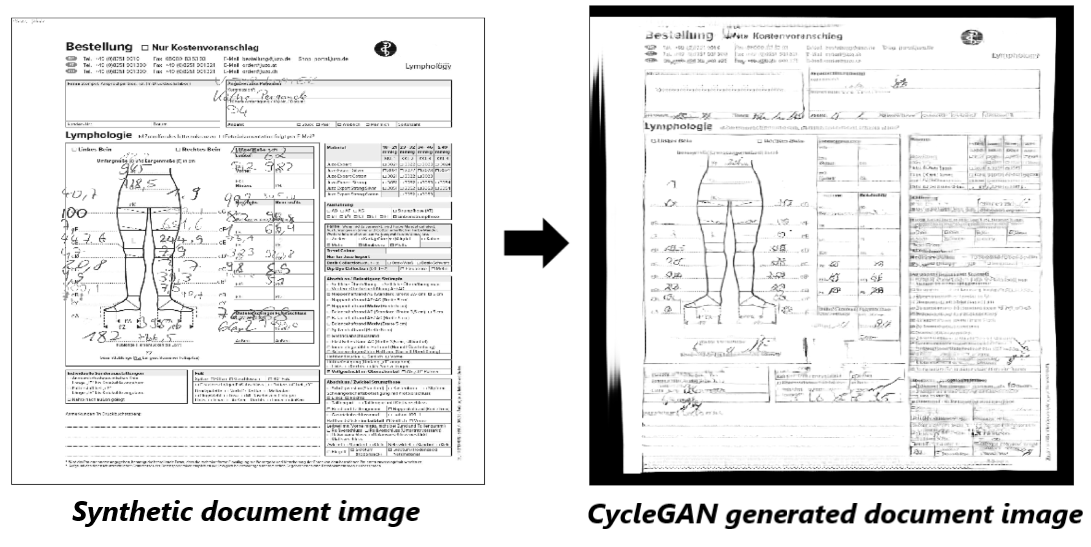
\includegraphics[scale=0.53]{images/Evaluation/failure3.png}
	    \caption[The \ac{CycleGAN} generated document image consists of dark border.]{The \ac{CycleGAN} generated document image consists of dark border (figure reproduced from elevait GmbH \& Co. KG with permission).}
	    \label{fig:failure3}
	    \end{center}
\end{figure}


\begin{figure}[H]
        \begin{center}
	    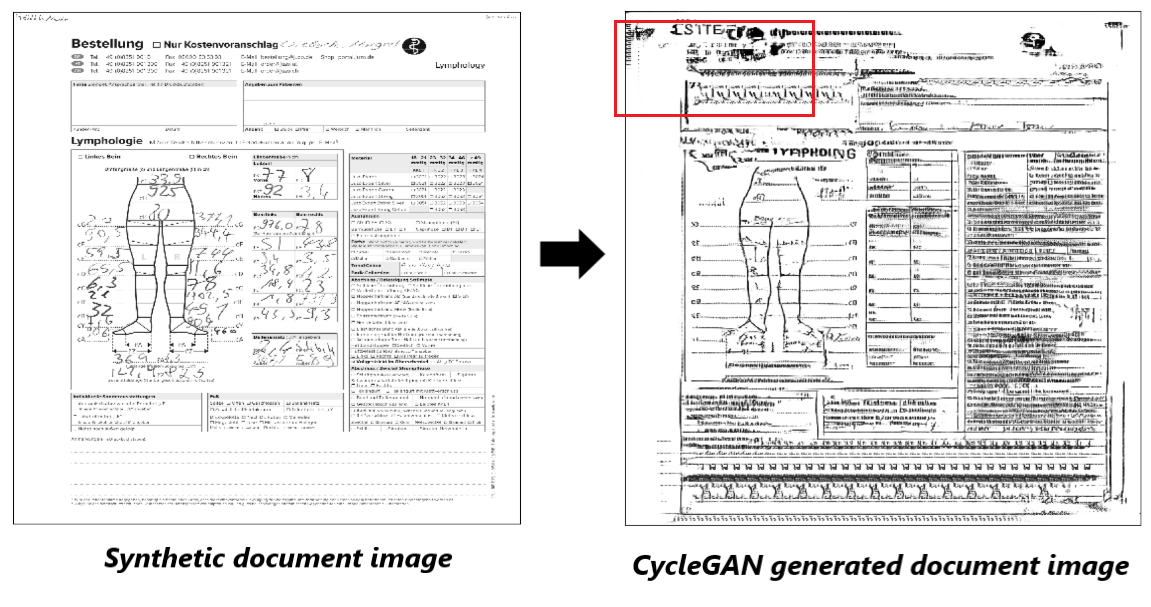
\includegraphics[scale=0.50]{images/Evaluation/failure4.png}
	    \caption[There are some artifacts appear in the generated image that are not present in the synthetic image.]{The \ac{CycleGAN} generated document image consists of noisy artifacts that are unrealistic and the visual quality of the generated image is not good. There are some artifacts (marked in red box) appear in the generated images that are not present in the synthetic image (figure reproduced from elevait GmbH \& Co. KG with permission).}
	    \label{fig:failure4}
	    \end{center}
\end{figure}






































%%%%%%%%%%%%%%%%%%%%%%%%%%%%%%%%%%%%%%%%%%%%%%%%%%%%%%%%%%%%%%%%%%%%%%%%%%%%%%%%%%%%%%%%%%%%%%%%%%%%%%%%%%%%%%%%%%%

%\subsection{Overview of Domain Gap between Distribution}
\begin{comment}
\begin{figure}[H]
        \begin{center}
	    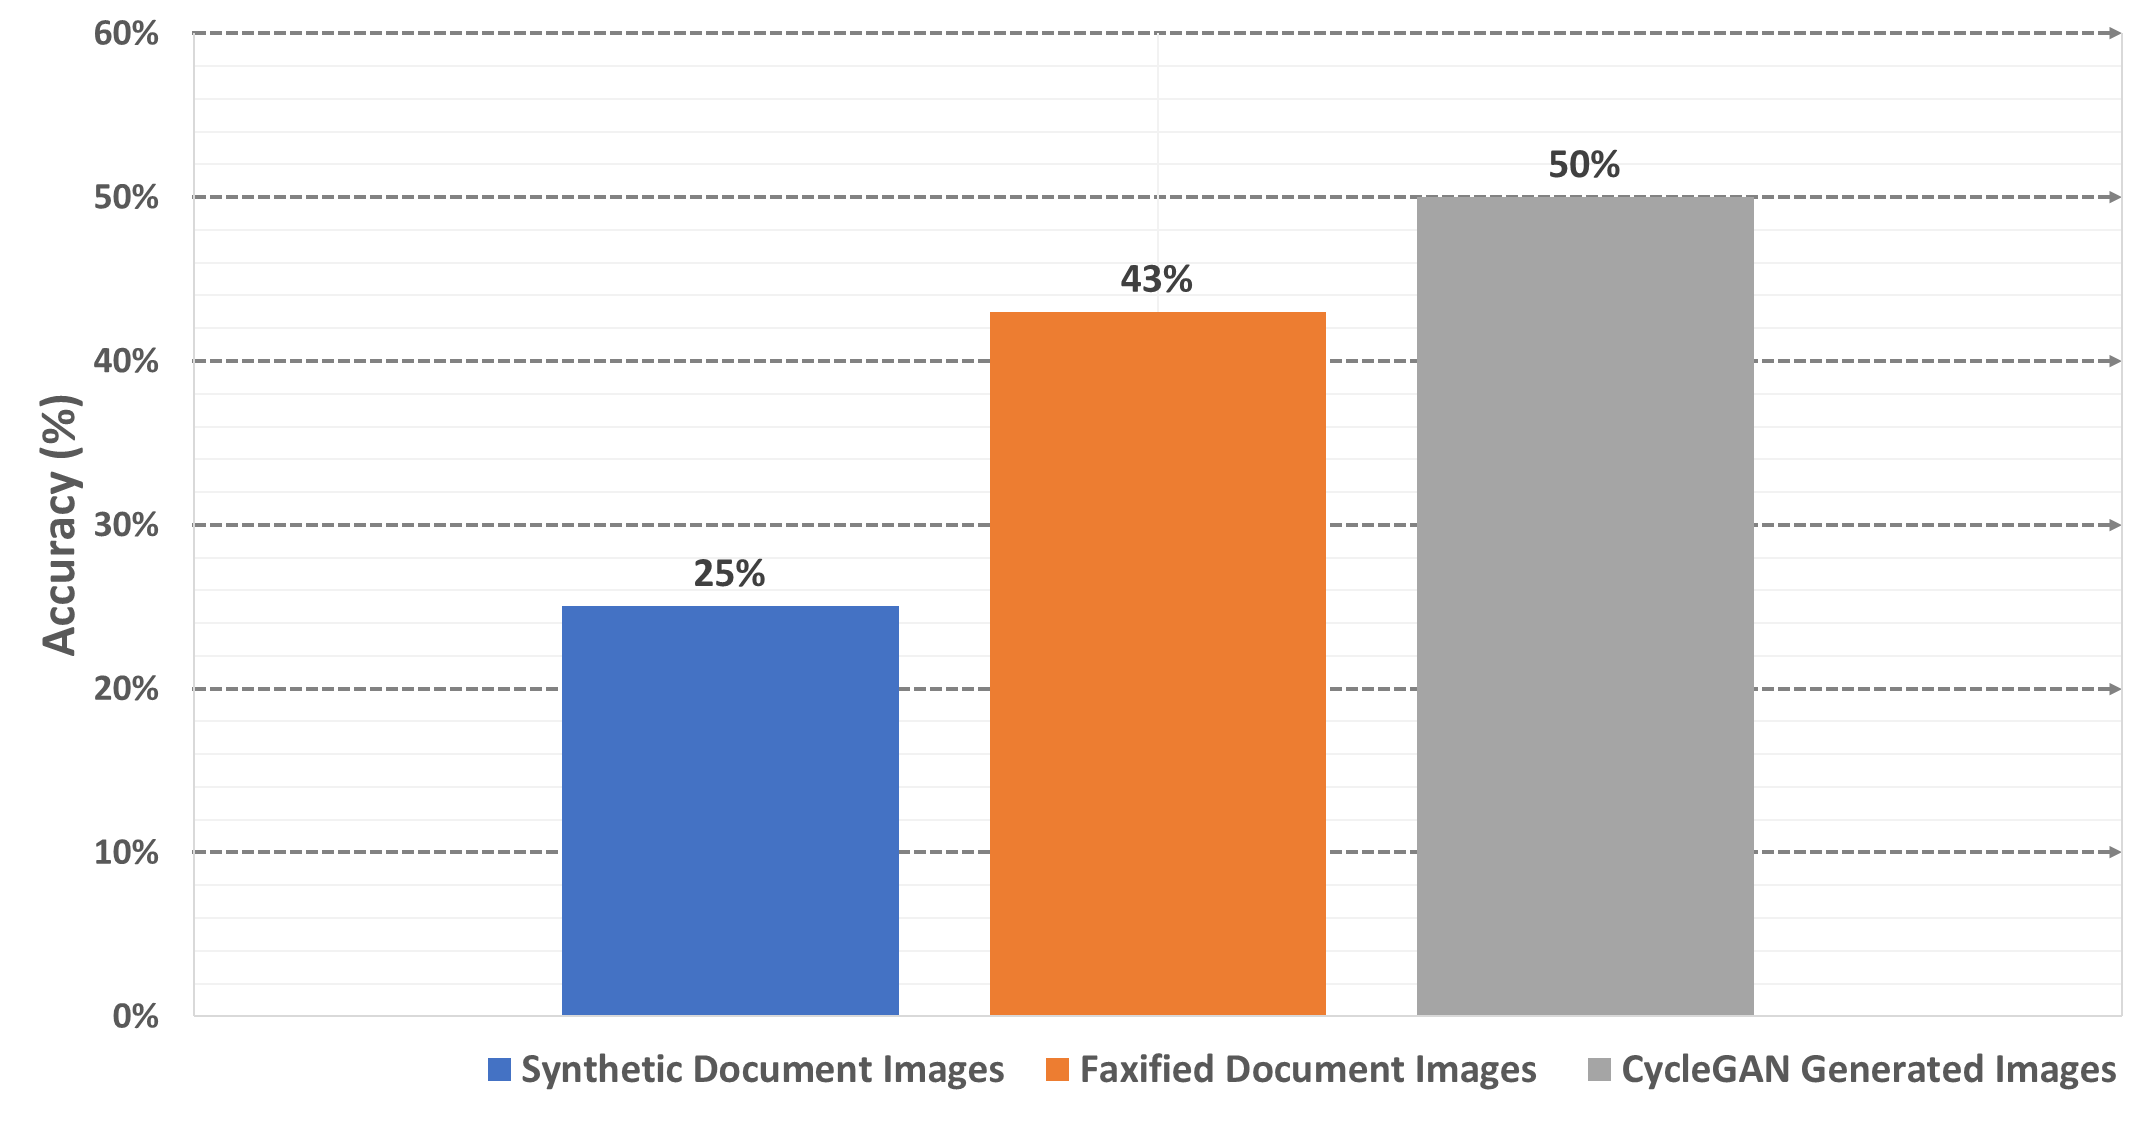
\includegraphics[scale=0.20]{images/DomainGap.png}
	    \caption[Illustration of Domain Gap Between Real Data Distribution and Synthetic Data Distribution, Faxified Data Distribution and \ac{CycleGAN} Generated Data Distribution.]{Illustration of Domain Gap Between Real Data Distribution and Synthetic Data Distribution, Faxified Data Distribution and \ac{CycleGAN} Generated Data Distribution. Initially, the classifiers are trained on Synthetic Document Images, Faxified Document Images and \ac{CycleGAN} Generated Document Images. Later their Classification Performance Evaluated on the Annotated Real Document Images to understand the Domain Gap between distributions using Accuracy as an Evaluation Metric.}
	    \label{fig:DomainGap}
	    \end{center}
\end{figure}
\end{comment}

%To evaluate the quality of images generated by the \ac{CycleGAN}, a classifier is trained on the \ac{CycleGAN} generated data and its accuracy on a real dtest dataset is used as a metric to measure how well the \ac{CycleGAN} model distribution matches the real data distribution. Basically, The classification capability of the trained classifier is used as an objective measure to assess the quality of images generated by \ac{CycleGAN}. Also, the classifier is trained on the synthetic document images and it's accuracy evaluated in 
%Classification report and metrics
%Three separate classifiers are trained upon synthetic data distribution, faxified data distribution and \ac{CycleGAN} generated data distribution respectively. After training the classifiers they have evaluated annotated real document images. Using this performance evaluation using metrics like weighted F1 score and accuracy 	


\begin{comment}
\begin{center}
\begin{table}[H]
    \begin{center}
    \begin{tabular}{P{0.30\linewidth} P{0.15\linewidth} P{0.20\linewidth} P{0.20\linewidth}} 
        \toprule
        \bf{Data Distributions} & \bf{Accuracy}  & \bf{Weighted average F1-score} & \bf{Macro average F1-score} \\[0.0ex] 
        \midrule
        \bf{Synthetic document images} & 25\% & 31\% & 27\%\\[0.0ex]
        \midrule
       \bf{\ac{CycleGAN} generated document images} & 27\% & 47\% &34\%\\[0.0ex]
        \midrule
        \bf{Faxified document images} & 43\% & 43\% & 58\%\\[0.0ex]
        \bottomrule
    \end{tabular}
    \caption[Comparison of accuracy and F1-scores when the classifiers trained on different data distributions and evaluated on annotated real document images.]{Comparison of accuracy and F1-scores when the classifiers trained on different data distributions and evaluated on annotated real document images.}
    \label{table:finalResults}
    \end{center}
\end{table}
\end{center}




\begin{center}
\begin{table}[H]
    \begin{center}
    \begin{tabular}{P{0.22\linewidth} P{0.22\linewidth} P{0.22\linewidth} P{0.22\linewidth}} 
        \toprule
        \bf{Classifier trained using} & \bf{Accuracy on annotated real document images}  & \bf{Weighted average F1-score on annotated real document images} & \bf{Macro average F1-score on annotated real document images} \\[0.0ex] 
        \midrule
        \bf{Synthetic document images} & 25\% & 31\% & 27\%\\[0.0ex]
        \midrule
       \bf{\ac{CycleGAN} generated document images} & 27\% & 47\% &34\%\\[0.0ex]
        \midrule
        \bf{Faxified document images} & 43\% & 43\% & 58\%\\[0.0ex]
        \bottomrule
    \end{tabular}
    \caption[Comparison of accuracy and F1-scores when the classifiers trained on different data distributions and evaluated on annotated real document images.]{Comparison of accuracy and F1-scores when the classifiers trained on different data distributions and evaluated on annotated real document images.}
    \label{table:finalResults}
    \end{center}
\end{table}
\end{center}



\begin{center}
\begin{table}[H]
    \begin{center}
    \begin{tabular}{P{0.35\linewidth} P{0.12\linewidth} P{0.20\linewidth} P{0.20\linewidth}} 
        \toprule
        \bf{Data distributions} & \bf{Accuracy}  & \bf{Weighted average F1-score} & \bf{Macro average F1-score} \\[0.0ex] 
	 \midrule
        \bf{Synthetic document images} & 25\% & 31\% & 27\%\\[0.0ex]
        \midrule
       \bf{\ac{CycleGAN} generated document images} & 27\% & 25\% & 34\%\\[0.0ex]
        \midrule
        \bf{Faxified document images} & 43\% & 43\% & 58\%\\[0.0ex]
        \bottomrule
    \end{tabular}
    \caption[Comparison of accuracy and F1-scores when the classifiers trained on different data distributions and evaluated on annotated real document images.]{Comparison of accuracy and F1-scores when the classifiers trained on different data distributions and evaluated on annotated real document images.}
    \label{table:finalResults}
    \end{center}
\end{table}
\end{center}

\begin{table}[H]
\hspace*{-5.40em}
\begin{tabular}{cccc} 
	\toprule
	\bf{Data distributions} & \bf{Accuracy}  & \bf{Weighted average F1-score} & \bf{Macro average F1-score} \\[0.0ex] 
	\midrule
     \bf{Synthetic document images} & 25\% & 31\% & 27\%\\[0.0ex]
     \midrule
     \bf{\ac{CycleGAN} generated document images} & 27\% & 25\% & 34\%\\[0.0ex]
     \midrule
     \bf{Faxified document images} & 43\% & 43\% & 58\%\\[0.0ex]
     \bottomrule
\end{tabular}
 \caption[The accuracies and F1-scores when the classifiers trained on different data distributions and evaluated on annotated real document images.]{The accuracies and F1-scores when the classifiers trained on different data distributions and evaluated on annotated real document images.}
    \label{table:finalResults}
\end{table}


\end{comment}